% =========================================================================== %
% This is the main file for the Eclipse Scout book.
% 
% The technical latex setup and organisation of the book heavily borrows from
% "Pharo by Example" https://github.com/SquareBracketAssociates/PharoByExample-english 
% 
% =========================================================================== %
\documentclass[a4paper,10pt,twoside]{book}

% --------------------------------------------------------------------------- %
% definitions etc. common to all sub content
% --------------------------------------------------------------------------- %
%=============================================================================%
% Common things, settings, packages to include
%=============================================================================%

\usepackage{graphicx}
\usepackage{color}
\usepackage{makeidx}
\usepackage{ifpdf}
\usepackage{verbatim}

% --------------------------------------------------------------------------- %
% Setting up stuff depeding on output format
% --------------------------------------------------------------------------- %

\ifpdf
  % special settings for pdf mode
  \usepackage[colorlinks]{hyperref}
  \usepackage{courier}
  
  \hypersetup{
    colorlinks,
    linkcolor=darkblue,
    citecolor=darkblue,
    pdftitle={The Eclipse Scout Book},
    pdfauthor={The Scout Community},
    pdfkeywords={Enterprise Framework, Eclipse, Java, Client-Side, Rich Client, Web Client, Mobile},
    pdfsubject={Computer Science}
  }
  
  \usepackage{caption}
  \captionsetup{margin=10pt,font=small,labelfont=bf}
\else
  % special stuff for html mode
  \usepackage[tex4ht]{hyperref}
\fi

% --------------------------------------------------------------------------- %
% Setting up printing range
% --------------------------------------------------------------------------- %

\parindent 1cm
\parskip 0.2cm
\topmargin 0.2cm
\oddsidemargin 1cm
\evensidemargin 0.5cm
\textwidth 15cm
\textheight 21cm

% --------------------------------------------------------------------------- %
% Setting up listings
% --------------------------------------------------------------------------- %

\usepackage{listings}
 
\definecolor{darkviolet}{rgb}{0.5,0,0.4}
\definecolor{darkgreen}{rgb}{0,0.4,0.2} 
\definecolor{darkblue}{rgb}{0.1,0.1,0.9}
\definecolor{darkgrey}{rgb}{0.5,0.5,0.5}
\definecolor{lightblue}{rgb}{0.4,0.4,1}
\definecolor{lightgray}{rgb}{0.97,0.97,0.97}

\renewcommand{\lstlistlistingname}{List of Listings}

% general settings
\lstset{
  basicstyle=\small\ttfamily,
  columns=fullflexible,
  breaklines=true,
  breakindent=10pt,
  prebreak=\mbox{{\color{blue}\tiny$\searrow$}},
  postbreak=\mbox{{\color{blue}\tiny$\rightarrow$}},
  showstringspaces=false,
  backgroundcolor=\color{lightgray}
}

% settings for xml files
\lstdefinelanguage{xml}
{
  commentstyle=\color{darkgrey}\upshape,
  morestring=[b]",
  morestring=[s]{>}{<},
  morecomment=[s]{<?}{?>},
  stringstyle=\color{black},
  identifierstyle=\color{darkblue},
  keywordstyle=\color{cyan},
  morekeywords={xmlns,name,point,factory,class}% list your attributes here
}

% settings for ini files
\lstdefinelanguage{ini}
{
  morecomment=[f][\color{darkgrey}\upshape][0]\#, % # is comment iff it's the first char on the line
  stringstyle=\color{black}
}

% default settings (for java files)
\lstset{
  language=Java,
  emphstyle=\color{red}\bfseries,
  keywordstyle=\color{darkviolet}\bfseries,
  commentstyle=\color{darkgreen},
  morecomment=[s][\color{lightblue}]{/**}{*/},
  stringstyle=\color{darkblue},
}

% --------------------------------------------------------------------------- %
% cross reference macros
% --------------------------------------------------------------------------- %
\newcommand{\applabel}[1]{\label{apx:#1}}
\newcommand{\chalabel}[1]{\label{cha:#1}}
\newcommand{\seclabel}[1]{\label{sec:#1}}
\newcommand{\lstlabel}[1]{\label{lst:#1}}
\newcommand{\figlabel}[1]{\label{fig:#1}}
\newcommand{\tablabel}[1]{\label{tab:#1}}

\newcommand{\appref}[1]{Appendix~\ref{apx:#1}}
\newcommand{\charef}[1]{Chapter~\ref{cha:#1}\xspace}
\newcommand{\secref}[1]{Section~\ref{sec:#1}}
\newcommand{\lstref}[1]{Listing~\ref{lst:#1}\xspace}
\newcommand{\figref}[1]{Figure~\ref{fig:#1}\xspace}
\newcommand{\tabref}[1]{Table~\ref{tab:#1}\xspace}

% --------------------------------------------------------------------------- %
% graphics paths
% --------------------------------------------------------------------------- %
\graphicspath{
  {figures/}
  {Introduction/figures/}
}

%=============================================================================%


% --------------------------------------------------------------------------- %
% graphics paths
% --------------------------------------------------------------------------- %
\graphicspath{
  {figures/}
  {modules/figures/}
  {Introduction/figures/}
  {ScoutRuntime/figures/}
  {ScoutTooling/figures/}
  {OneDayTutorial/figures/}
  {ScoutClient/figures/}
  {ScoutInstallation/figures/}  
  {EclipseBasics/figures/}  
}

\let\wholebook=\relax
\makeindex

% --------------------------------------------------------------------------- %
% use this if you are working on individual chapters
% --------------------------------------------------------------------------- %
% \includeonly{Introduction/Introduction}
% \includeonly{ScoutRuntime/ScoutRuntime}

% =========================================================================== %
% Start content of book
% for usage of frontmatter etc. see
% http://tex.stackexchange.com/questions/20538/what-is-the-right-order-when-using-tableofcontents-frontmatter-mainmatter
% =========================================================================== %
\begin{document}

\ifpdf
  
\includepdf[pages=-]{ScoutBookCoverIntro.pdf}
\else
  
\includegraphics{ScoutBookCoverIntro.png}
\fi

\thispagestyle{empty}
\frontmatter

% --------------------------------------------------------------------------- %
% Title page, copyright, table of contents, preface
% --------------------------------------------------------------------------- %

%=============================================================================%
% The title page
%=============================================================================%

\author{Matthias Zimmermann}
\title{
\Huge\bf Eclipse Scout\\
\huge An Introduction
}
\ifpdf
  \isodate
\fi
\date{\emph{Version of \today}}
\maketitle

%=============================================================================%


\pagenumbering{roman}
\pagestyle{plain}

\tableofcontents
\sloppy

% =========================================================================== %
% Preface
% please make sure that this fits into two pages (max)
% =========================================================================== %

\ifx\wholebook\relax\else
  \documentclass[a4paper,10pt,twoside]{book}
  %=============================================================================%
% Common things, settings, packages to include
%=============================================================================%

\usepackage{graphicx}
\usepackage{color}
\usepackage{makeidx}
\usepackage{ifpdf}
\usepackage{verbatim}

% --------------------------------------------------------------------------- %
% Setting up stuff depeding on output format
% --------------------------------------------------------------------------- %

\ifpdf
  % special settings for pdf mode
  \usepackage[colorlinks]{hyperref}
  \usepackage{courier}
  
  \hypersetup{
    colorlinks,
    linkcolor=darkblue,
    citecolor=darkblue,
    pdftitle={The Eclipse Scout Book},
    pdfauthor={The Scout Community},
    pdfkeywords={Enterprise Framework, Eclipse, Java, Client-Side, Rich Client, Web Client, Mobile},
    pdfsubject={Computer Science}
  }
  
  \usepackage{caption}
  \captionsetup{margin=10pt,font=small,labelfont=bf}
\else
  % special stuff for html mode
  \usepackage[tex4ht]{hyperref}
\fi

% --------------------------------------------------------------------------- %
% Setting up printing range
% --------------------------------------------------------------------------- %

\parindent 1cm
\parskip 0.2cm
\topmargin 0.2cm
\oddsidemargin 1cm
\evensidemargin 0.5cm
\textwidth 15cm
\textheight 21cm

% --------------------------------------------------------------------------- %
% Setting up listings
% --------------------------------------------------------------------------- %

\usepackage{listings}
 
\definecolor{darkviolet}{rgb}{0.5,0,0.4}
\definecolor{darkgreen}{rgb}{0,0.4,0.2} 
\definecolor{darkblue}{rgb}{0.1,0.1,0.9}
\definecolor{darkgrey}{rgb}{0.5,0.5,0.5}
\definecolor{lightblue}{rgb}{0.4,0.4,1}
\definecolor{lightgray}{rgb}{0.97,0.97,0.97}

\renewcommand{\lstlistlistingname}{List of Listings}

% general settings
\lstset{
  basicstyle=\small\ttfamily,
  columns=fullflexible,
  breaklines=true,
  breakindent=10pt,
  prebreak=\mbox{{\color{blue}\tiny$\searrow$}},
  postbreak=\mbox{{\color{blue}\tiny$\rightarrow$}},
  showstringspaces=false,
  backgroundcolor=\color{lightgray}
}

% settings for xml files
\lstdefinelanguage{xml}
{
  commentstyle=\color{darkgrey}\upshape,
  morestring=[b]",
  morestring=[s]{>}{<},
  morecomment=[s]{<?}{?>},
  stringstyle=\color{black},
  identifierstyle=\color{darkblue},
  keywordstyle=\color{cyan},
  morekeywords={xmlns,name,point,factory,class}% list your attributes here
}

% settings for ini files
\lstdefinelanguage{ini}
{
  morecomment=[f][\color{darkgrey}\upshape][0]\#, % # is comment iff it's the first char on the line
  stringstyle=\color{black}
}

% default settings (for java files)
\lstset{
  language=Java,
  emphstyle=\color{red}\bfseries,
  keywordstyle=\color{darkviolet}\bfseries,
  commentstyle=\color{darkgreen},
  morecomment=[s][\color{lightblue}]{/**}{*/},
  stringstyle=\color{darkblue},
}

% --------------------------------------------------------------------------- %
% cross reference macros
% --------------------------------------------------------------------------- %
\newcommand{\applabel}[1]{\label{apx:#1}}
\newcommand{\chalabel}[1]{\label{cha:#1}}
\newcommand{\seclabel}[1]{\label{sec:#1}}
\newcommand{\lstlabel}[1]{\label{lst:#1}}
\newcommand{\figlabel}[1]{\label{fig:#1}}
\newcommand{\tablabel}[1]{\label{tab:#1}}

\newcommand{\appref}[1]{Appendix~\ref{apx:#1}}
\newcommand{\charef}[1]{Chapter~\ref{cha:#1}\xspace}
\newcommand{\secref}[1]{Section~\ref{sec:#1}}
\newcommand{\lstref}[1]{Listing~\ref{lst:#1}\xspace}
\newcommand{\figref}[1]{Figure~\ref{fig:#1}\xspace}
\newcommand{\tabref}[1]{Table~\ref{tab:#1}\xspace}

% --------------------------------------------------------------------------- %
% graphics paths
% --------------------------------------------------------------------------- %
\graphicspath{
  {figures/}
  {Introduction/figures/}
}

%=============================================================================%

	\pagestyle{headings}
  \graphicspath{{figures/} {../figures/}}
  \begin{document}
  \sloppy
\fi


% --------------------------------------------------------------------------- %
\chapter{Preface}

Today, the Java platform is widely seen as the primary choice for implementing enterprise applications. 
While many successful frameworks support the development of persistence layers and business services, implementing front-ends in a simple and clean way remains a challenge. 
This is exactly where Eclipse Scout fits in. 
The primary goal of Scout is to make your life as a developer easier and to help organisations to save money and time. 
For this, the Scout framework covers most of the recurring front-end aspects such as user authentication, client-server communication and the user interface. 
This comprehensive scope reduces the amount of necessary boiler plate code, and let developers concentrate on understanding and implementing business functionality. 

The purpose of this book is to get the reader familiar with the Scout framework.
In this book Scout's core features are introduced and explained using many practical examples. 
And as both the Scout framework and Scout applications are written in Java, we make the assumption that you are familiar with the language too. 
Ideally, you have worked with Java for some time now and feel comfortable with the basic language features. 

In the first part of the book a general introduction into the runtime part of the framework and the tooling - the Scout SDK - is provided. 
After the mandatory ''Hello World!'' application, the book walks you though a complete client server application including database access. 
The focus of the book's second part is on the front-end side of Scout applications. 
First, an overview of the Scout client model is introduced before Scout's most important UI components are described based on the Scout widget demo application. 
To cover the the server-side of Scout applications, an additional part of the book is planned to be released jointly with version 5.0 of the Scout framework. 
And finally, we intend to amend the book regarding building, testing and continuous integration for Scout applications. 

Last but not least, we thank you for your interest in Scout, for being part of our community and for your friendly support of new community members.
To allow for contributions to this book, the technical setup and the book's licence have been selected to minimize restrictions. 
According to the terms of the Creative Commons (CC-BY) license, you are allowed to freely use, share and adapt this book. 
All source files of the book including the Scout projects described in the book are available on github.
For the first edition of this book, we did already receive a number of bug reports and comments that were pointing out mistakes, inconsistencies and suggestions for changes. 
This feedback is very valuable to us as it helps to improve both the book's content and the quality for all future readers. 
We hope that this book helps you to get started quickly and would love to get your feedback. 

% --------------------------------------------------------------------------- %

\ifx\wholebook\relax\else
   \begin{thebibliography}{99}
  \addcontentsline{toc}{chapter}{Bibliography}
  
  % add/insert books in alphabetical order of 1st author
  
  \bibitem{batessierra05}
    \textit{Bert Bates, Kathy Sierra},
	\textbf{Head First Java} 2nd edition, 
	O'Reilly Media, 2005.

  \bibitem{bloch08} 
    \textit{Joshua Bloch},
    \textbf{Effective Java} 2nd edition, 
	Addison-Wesley, 2008.
	
  \bibitem{eckel06}
    \textit{Bruce Eckel},
	\textbf{Thinking in Java} 4th edition, 
	Prentice Hall International, 2006.

\end{thebibliography}

   \end{document}
\fi

% =========================================================================== %

\mainmatter

% =========================================================================== %
% Main content of book starts here
% =========================================================================== %

\pagestyle{headings}
\pagenumbering{arabic}

% --------------------------------------------------------------------------- %
% =========================================================================== %
% Introduction
% =========================================================================== %

\ifx\wholebook\relax\else
  \documentclass[a4paper,10pt,twoside]{book}
  %=============================================================================%
% Common things, settings, packages to include
%=============================================================================%

\usepackage{graphicx}
\usepackage{color}
\usepackage{makeidx}
\usepackage{ifpdf}
\usepackage{verbatim}

% --------------------------------------------------------------------------- %
% Setting up stuff depeding on output format
% --------------------------------------------------------------------------- %

\ifpdf
  % special settings for pdf mode
  \usepackage[colorlinks]{hyperref}
  \usepackage{courier}
  
  \hypersetup{
    colorlinks,
    linkcolor=darkblue,
    citecolor=darkblue,
    pdftitle={The Eclipse Scout Book},
    pdfauthor={The Scout Community},
    pdfkeywords={Enterprise Framework, Eclipse, Java, Client-Side, Rich Client, Web Client, Mobile},
    pdfsubject={Computer Science}
  }
  
  \usepackage{caption}
  \captionsetup{margin=10pt,font=small,labelfont=bf}
\else
  % special stuff for html mode
  \usepackage[tex4ht]{hyperref}
\fi

% --------------------------------------------------------------------------- %
% Setting up printing range
% --------------------------------------------------------------------------- %

\parindent 1cm
\parskip 0.2cm
\topmargin 0.2cm
\oddsidemargin 1cm
\evensidemargin 0.5cm
\textwidth 15cm
\textheight 21cm

% --------------------------------------------------------------------------- %
% Setting up listings
% --------------------------------------------------------------------------- %

\usepackage{listings}
 
\definecolor{darkviolet}{rgb}{0.5,0,0.4}
\definecolor{darkgreen}{rgb}{0,0.4,0.2} 
\definecolor{darkblue}{rgb}{0.1,0.1,0.9}
\definecolor{darkgrey}{rgb}{0.5,0.5,0.5}
\definecolor{lightblue}{rgb}{0.4,0.4,1}
\definecolor{lightgray}{rgb}{0.97,0.97,0.97}

\renewcommand{\lstlistlistingname}{List of Listings}

% general settings
\lstset{
  basicstyle=\small\ttfamily,
  columns=fullflexible,
  breaklines=true,
  breakindent=10pt,
  prebreak=\mbox{{\color{blue}\tiny$\searrow$}},
  postbreak=\mbox{{\color{blue}\tiny$\rightarrow$}},
  showstringspaces=false,
  backgroundcolor=\color{lightgray}
}

% settings for xml files
\lstdefinelanguage{xml}
{
  commentstyle=\color{darkgrey}\upshape,
  morestring=[b]",
  morestring=[s]{>}{<},
  morecomment=[s]{<?}{?>},
  stringstyle=\color{black},
  identifierstyle=\color{darkblue},
  keywordstyle=\color{cyan},
  morekeywords={xmlns,name,point,factory,class}% list your attributes here
}

% settings for ini files
\lstdefinelanguage{ini}
{
  morecomment=[f][\color{darkgrey}\upshape][0]\#, % # is comment iff it's the first char on the line
  stringstyle=\color{black}
}

% default settings (for java files)
\lstset{
  language=Java,
  emphstyle=\color{red}\bfseries,
  keywordstyle=\color{darkviolet}\bfseries,
  commentstyle=\color{darkgreen},
  morecomment=[s][\color{lightblue}]{/**}{*/},
  stringstyle=\color{darkblue},
}

% --------------------------------------------------------------------------- %
% cross reference macros
% --------------------------------------------------------------------------- %
\newcommand{\applabel}[1]{\label{apx:#1}}
\newcommand{\chalabel}[1]{\label{cha:#1}}
\newcommand{\seclabel}[1]{\label{sec:#1}}
\newcommand{\lstlabel}[1]{\label{lst:#1}}
\newcommand{\figlabel}[1]{\label{fig:#1}}
\newcommand{\tablabel}[1]{\label{tab:#1}}

\newcommand{\appref}[1]{Appendix~\ref{apx:#1}}
\newcommand{\charef}[1]{Chapter~\ref{cha:#1}\xspace}
\newcommand{\secref}[1]{Section~\ref{sec:#1}}
\newcommand{\lstref}[1]{Listing~\ref{lst:#1}\xspace}
\newcommand{\figref}[1]{Figure~\ref{fig:#1}\xspace}
\newcommand{\tabref}[1]{Table~\ref{tab:#1}\xspace}

% --------------------------------------------------------------------------- %
% graphics paths
% --------------------------------------------------------------------------- %
\graphicspath{
  {figures/}
  {Introduction/figures/}
}

%=============================================================================%

  \pagestyle{headings}
  \graphicspath{{figures/} {../figures/}}
  \begin{document}
  \sloppy
\fi


% =========================================================================== %
\chapter{Introduction}

% --------------------------------------------------------------------------- %
\section{What is Scout?}

Scout is a mature framework for building business applications. 
With its multi-frontend support, a single Scout applications may run as a desktop application, in a web browser or on a mobile phone with touch support. 
The clean separation of Scout's client model from the user interface technologies allows the developer to concentrate on a single code base. 
This approach has advantages for end users of Scout applications, Scout developers, and organisations implementing Scout applications.
In the text below we will explain Scout from the perspective of these three roles.

% ........................................................................... %
\subsection{End User Perspective}

End users of enterprise applications typically care about friendly user interfaces (UI) and well designed functionality that support them in doing their job.
Depending on the role and the current context of an end users, either mobile, web or desktop clients work best.
In the text below, we use a real world enterprise application to highlight how Scout applications can provide user friendly UIs on the desktop, in the browser and on mobile phones.

\begin{figure}
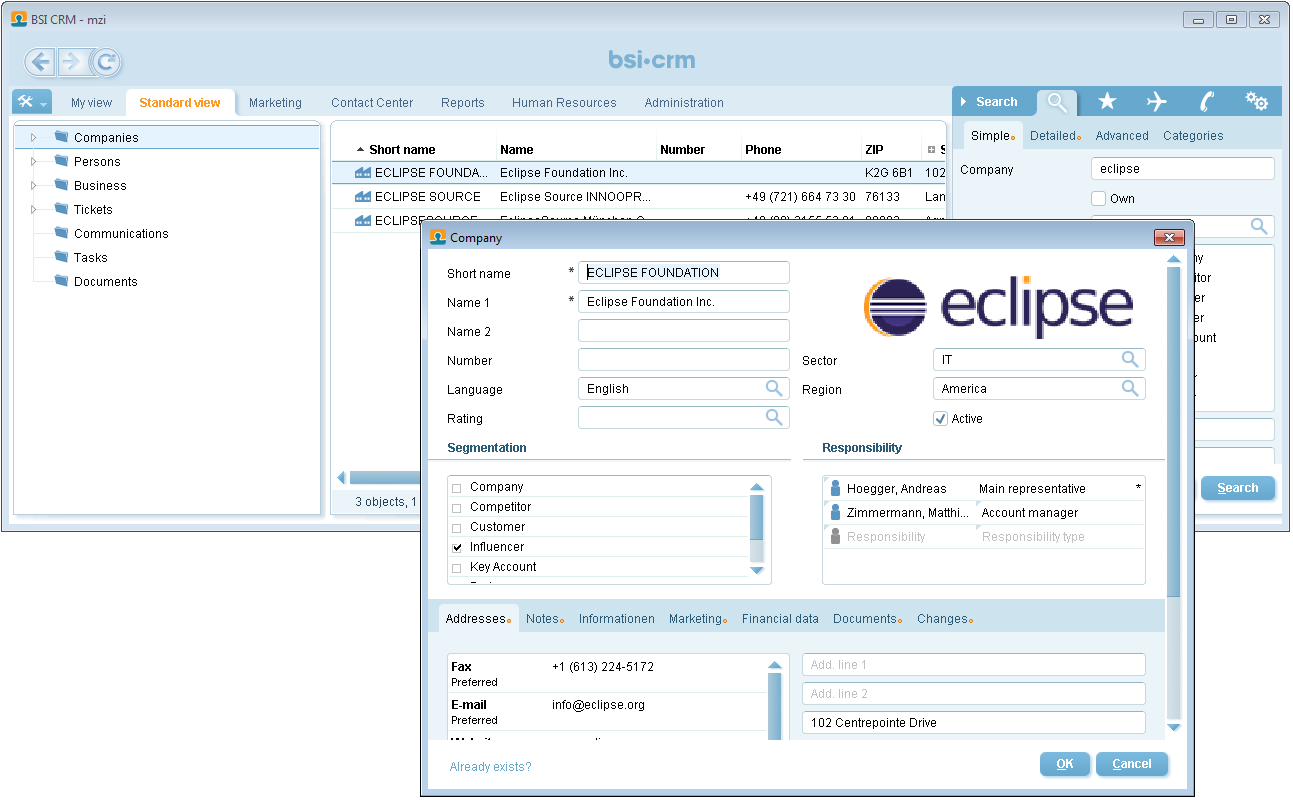
\includegraphics[width=14cm]{bsi_crm_desktop.png}
\caption{The desktop client of a Scout enterprise application.}
\figlabel{bsi_crm_desktop}
\end{figure}

If the user is working from a desk and frequently engaged in customer calls, good integration with locally installed software such as Lotus Notes or Microsoft Office products can significantly boost productivity.
So far, such a scenario still requires a desktop client application.
An example screenshot of a Scout desktop client application from a customer relationship management (CRM) solution is provided in \figref{bsi_crm_desktop}.
The screenshot provides a good overview of the general layout of the application.
On the left side a tree for simple navigation through the available entities, such as companies, persons and communications is provided.
Once an entity is selected, a click on the magnifying glass opens a search form on the right hand side.
In this search form a number of search fields is provided.
After entering ''eclipse'' into the company search field -- and clicking the search button at the bottom of the search form -- the list of matching entries is presented to the user.
With a right mouse click on the desired row, the corresponding company dialog can be opened for editing.

\begin{figure}
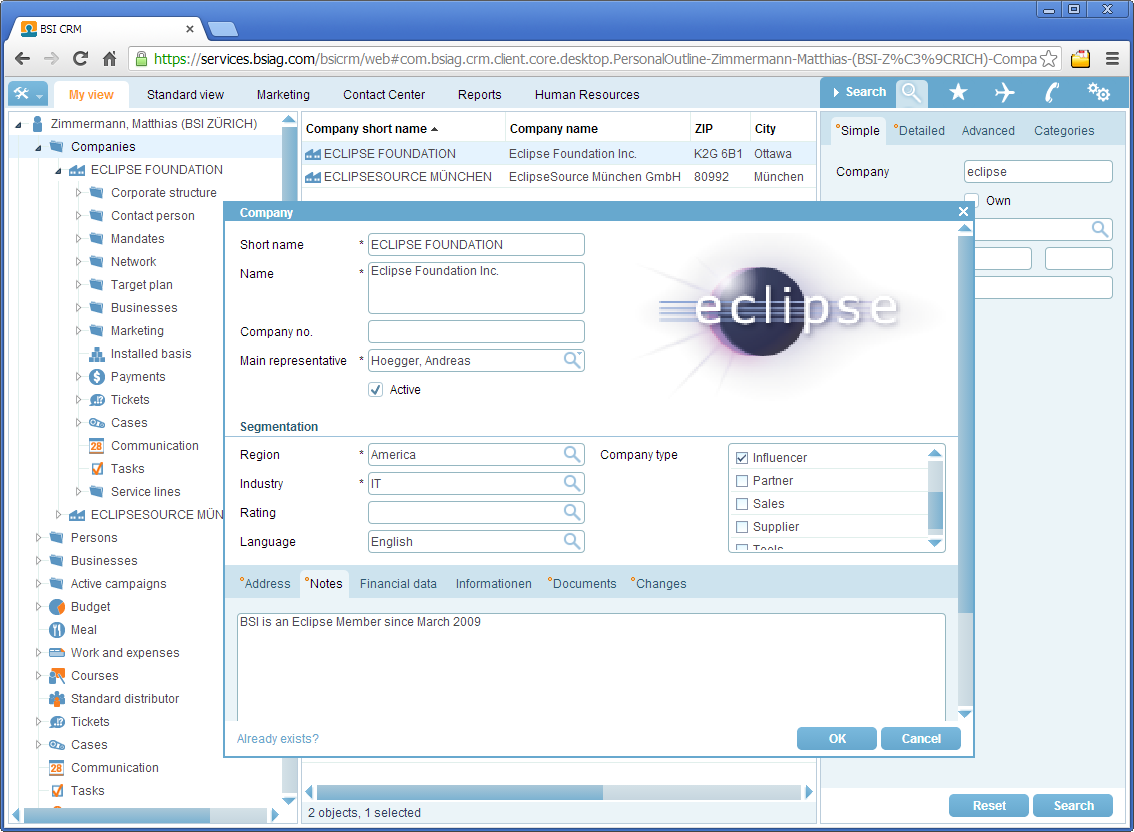
\includegraphics[width=14cm]{bsi_crm_web.png}
\caption{A Scout enterprise application running in a web browser.}
\figlabel{bsi_crm_web}
\end{figure}

When a user needs to work from a computer that does not have a desktop client installed (or lacks the time or the necessary permission to install software) the natural choice is to work with a web application.
As Scout offers multi-frontend capabilities out of the box, a web frontend can easily be provided for Scout business applications.
The primary benefits of Scout web applications for end users are a consistent look and feel and behaviour for both the web client and the desktop client.
In \figref{bsi_crm_web} a screenshot of the web client of the CRM Scout application is shown.

\begin{figure}
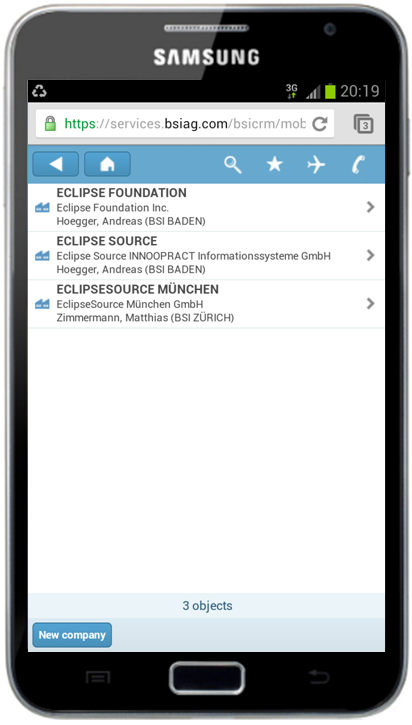
\includegraphics[width=7cm]{bsi_crm_mobile_galaxy.png}
\caption{The same Scout enterprise application running on a mobile device.}
\figlabel{bsi_crm_mobile}
\end{figure}

Often, user find themselves in meetings or on the move where it is not possible to work with desktop or laptop computers.
In such situations, accessing applications via tablets or mobile phones is the only meaningful approach.
As shown in \figref{bsi_crm_mobile}, a screenshot of the familiar CRM application is provided.
The user still benefits from the familiar look and feel and the known functionality of the application.

In contrast to desktop and web applications, most tablets and mobile phones are controlled using touch features instead of mouse clicks.
In addition, less elements may be presented on a single screen compared to desktop devices.
These two aspects makes it impractical to directly reuse the desktop user interface on mobile devices.
Using the Scout mobile extension, the user interface of Scout applications can be transformed on the fly to adapt to touch control and the smaller form factor of mobile devices.
This transformation can be observed when comparing the company table shown in the background of \figref{bsi_crm_desktop} with the company list presented in \figref{bsi_crm_mobile}.
The multi-column table of the desktop client has been transformed into a list providing the content of the first few table columns on separate rows.
In addition, the context menu ''New company'' is now provided as a touch button.
As the navigation in the application and the offered choices remain the same for Scout desktop and mobile applications, the end user feels immediately comfortable working with Scout mobile applications.

% ........................................................................... %
\subsection{Management Perspective}

For the management, Scout is best explained in terms of benefits it brings to the organisation in question. 
This is why we are going to concentrate on a (typical) application migration scenario here. 
Let us assume that to support the company's business, a fairly large landscape of multi-tier applications has to be maintained and developed. 
Including host systems, client server applications including desktop clients, as well as newer web based applications. 

\begin{figure}
\includediagram{14cm}{scout_with_other_apps}
\caption{A typical application landscape including a service bus and a Scout application.}
\figlabel{scout_with_other_apps}
\end{figure}

Usually, these applications interact with each other through a service bus as shown in \figref{scout_with_other_apps}. 
Often, some of the applications that are vital to the organisation's core business have grown historically and are based on legacy technologies. 
And for technologies that are no longer under active development it can get difficult to find staff having the necessary expertise or motivation. 
Sometimes, the organisation is no longer willing to accept the costs and technology risks of such mission critical applications. 

\begin{figure}
\includediagram{14cm}{scout_integration}
\caption{The integration of a Scout application in a typical enterprise setup.}
\figlabel{scout_integration}
\end{figure}

In this situation, the company needs to evaluate if it should buy a new standard product or if the old application has to be migrated to a new technology stack. 
Now let us assume, that available products do not fit the company's requirements well enough and we have to settle for the migration scenario.
In the target architecture, a clean layering similar to the one shown in \figref{scout_integration} is often desirable.

While a number of modern and established technologies exist that address the backend side (data bases, data access and business services), the situation is different for the UI layer and the application layer. 
The number of frameworks to develop web applications with Java is excessively large\footnote{
Web application framework comparison: \url{http://en.wikipedia.org/wiki/Comparison_of_web_application_frameworks#Java}.
},
but the choice between desktop application technologies in the Java domain is restricted to three options only. 
Swing, SWT and JavaFX.
Both Eclipse SWT and Java Swing are mature and well established but Swing is moving into 'maintenance only' mode and will be replaced by JavaFX.
However, the maturity of the new JavaFX technology in large complex enterprise applications is not yet established. 
Obviously, deciding for the right UI technology is a challenge and needs to be made very carefully. 
Reverting this decision late in a project or after going into production can get very expensive and time consuming. 

Once the organisation has decided for a specific UI technology, additional components and frameworks need to be evaluated to cover client server communication, requirements for the application layer, and integration into the existing application landscape. 
To avoid drowning in the integration effort for all the elements necessary to cover the UI and the application layer a 'lightweight' framework is frequently developed. 
When available, this framework initially leads to desirable gains in productivity. 
Unfortunately, such frameworks often become legacy by themselves. 
Setting up a dedicated team to actively maintain the framework and adapt to new technologies can reduce this risk. 
But then again, such a strategy is expensive and developing business application frameworks is usually not the core business of a company. 

Can we do better? 
To implement a business application that covers the UI and the application layer as shown in \figref{scout_integration}, Eclipse Scout substantially reduces both risk and costs compared to the inhouse development presented above.
First or all, Scout is completely based on Java and Eclipse. 
Chances are, that developers are already familiar with some of these technologies.
This helps in getting developers up to speed and keeping training costs low. 

On the UI side, Scout's multi-frontend support almost allows to skip the decision for a specific UI technology. 
Should a particular web framework become the de-facto standard in the next years, it will be the responsibility of the Scout framework to provide the necessary support. 
Existing Scout applications can then switch to this new technology with only minimal effort. 
This is possible because the Scout developers are designing and building the UI of an application using Scout's client model.
And this client model is not linked to any specific UI technology. 
Rather, specific UI renderers provided by the Scout framework are responsible to draw the UI at runtime. 

As Scout is an open source project, no licence fees are collected. 
Taking advantage of the growing popularity of Scout, free community support is available via a dedicated forum. 
At the same time, professional support is available if the organisation decides for it.

As the migration of aging applications to current technology is always a challenge, it surely helps to have Scout in the technology portfolio. 
Not only is it a low risk choice, but also boosts developer productivity and helps to motivate the development team. 
Additional reasons on why Scout helps to drive down cost and risks are discussed in \secref{why_scout}.

% ........................................................................... %
\subsection{Developer Perspective}

From the perspective of application developers, Scout offers a Java based framework that covers the complete client server architecture. 
This implies that -- once familiar with the Scout framework -- the developer can concentrate on a single framework language (Java) and a single set of development tools. 

As Scout is completely based on Java and Eclipse, Scout developers can take full advantage of existing knowledge and experience in these domains. 
And to make learning Scout as simple as possible, Scout includes a comprehensive software development kit (SDK), the Scout SDK.
The Scout SDK helps to create a robust initial project setup for client server applications and includes a large set of wizards for repetitive and error prone tasks.

On the client-side Scout's flexible client model allows the developer to create a good user experience without having to care about specific UI technologies. 
The reason for this can be found in Scout's client architecture that cleanly separates the UI model from the UI technology.
In Scout (almost) every UI component is implemented four times. 
First the implementation of the UI model component and then, three rendering components for each UI technology supported by Scout. 
For desktop clients these are the Swing and the SWT technologies, and for the web and mobile support this is Eclipse RAP which in turn takes care of the necessary JavaScript parts.  

Not having to worry about Swing, SWT or JavaScript can significantly boost the productivity.
With one exception. 
If a specific UI widget is missing for the user story to be implemented, the Scout developer first needs to implement such a widget. 
Initially, this task is slightly more complex than not working with Scout. 
For custom widgets the Scout developer needs to implement both a model component and a rendering component for a specific UI technology. 
But as soon as the client application needs to be available on more than a single frontend, the investment already pays off.
The developer already did implement the model component and only needs to provide an additional rendering component for the new UI technology.
In most situations the large set of Scouts UI components provided out-of-the box are sufficient and user friendly applications are straight forward to implement. 
Even if the application needs to run on different target devices simultaneously.

Client-server communication is an additional aspect where the developers is supported by Scout.
Calling remote services in the client application that are provided by the Scout server looks identical to the invocation of local services. 
The complete communication including the transfer of parameter objects is handled fully transparent by the Scout framework.
In addition, the Scout SDK can completely manage the necessary transfer objects to fetch data from the Scout server that is to be shown in dialog forms on the Scout client.
The binding of the transferred data to the form fields is done by the framework.

Although the Scout SDK wizards can generate a significant amount of code, there is no one-way code generation and no meta data in a Scout application.
Just the Java code\footnote{
With the exception of the \filename{plugin.xml} and \filename{MANIFEST.MF} files required for Eclipse plugins.
}. 
Developers preferring to write the necessary code manually, may do so. 
The Scout SDK parses the application's Java code in the background to present the updated Scout application model to the developers preferring to work with the Scout SDK. 

TODO What should we focus on the server side? transaction handling, services, ...? 

Finally, Scout is an open source framework hosted at the Eclipse foundation. 
This provides a number of interesting options to developers that are not available for closed source frameworks. 
First of all, it is simple to get all the source code of Scout and the underlying Eclipse platform. 
This allows for complete debugging of all problems and errors found in Scout applications. 
Starting from the application code, including the Scout framework, Eclipse and down to the Java platform. 

Scout developer can also profit from an increasing amount of free and publicly available documentation, such as this book or the Scout Wiki pages. 
And problems with Scout or questions that are not clearly addressed by existing documentation can be discussed in the Scout forum. 
The forum is also a great place for Scout developers to help out in tricky situation and learn from others. 
Ideally, answered questions lead to improved or additional documentation in the Scout Wiki.

At times, framework bugs can be identified from questions asked in the forum. 
As all other enhancement requests and issues, such bugs can be reported in Bugzilla by the Scout developer. 
Using Bugzilla, Scout developers can also contribute bug analysis and patch proposals to solve the reported issue.
With this process, Scout developers can actively contribute to the code base of Eclipse Scout.
This has the advantage, that workarounds in existing Scout applications can be removed when an upgrade of the Scout framework is made.

Having provided a significant number of high quality patches and a meaningful involvement in the Scout community, the Scout project can nominate a Scout developer as a new Scout committer. 
Fundamentally, such a nomination is based on the trust of Scout committers in the candidate. 
To quote the official guidelines\footnote{
Nominating and electing a new Eclipse Scout committer: \url{http://wiki.eclipse.org/Development_Resources/HOWTO/Nominating_and_Electing_a_New_Committer#Guidelines_for_Nominating_and_Electing_a_New_Committer}.
} 
for nominating and electing a new committer:

\begin{quotation}
\begin{em}
A Committer gains voting rights allowing them to affect the future of the Project. 
Becoming a Committer is a privilege that is earned by contributing and showing discipline and good judgment. 
It is a responsibility that should be neither given nor taken lightly, nor is it a right based on employment by an Eclipse Member company or any company employing existing committers.
\end{em}
\end{quotation}

\noindent After a successful election process (existing committers voting for and not against the candidate) the Scout developer effectively becomes a Scout committer. 
With this new status, the Scout developer then gets write access to the Eclipse Scout repositories and gains voting rights and the possibility to shape the future of Scout. 

% --------------------------------------------------------------------------- %
\section{Why should I choose Scout?}
\seclabel{why_scout}

Protect your investment
\begin{itemize}
  \item Scout is proven in production for more than 10 years
  \item Scout is based on Java and the Eclipse platform
  \item Scout is an open source project hosted at the Eclipse foundation
  \item Scout has an active and growing community
  \item Scout is moving with the best available technologies.

\end{itemize}

Lower your cost for inhouse applications (Money)
\begin{itemize}
  \item Increase your development productivity with Scout
  \item Take advantage of low maintenance costs for Scout applications
  \item Leverage existing experience in Java
\end{itemize}

Run your app on any device (desktop, tablet, mobile phone)
\begin{itemize}
  \item Scout developers implement the application model only
  \item In Scout, the user interface is modeled independently of any specific UI technology
  \item At runtime, the user interface is rendered using a specific Scout UI plugin
  \item For desktop apps, choose SWT or Swing
  \item For browser or mobile apps, choose RAP
\end{itemize}

Get up to speed in days (5' clock)
\begin{itemize}
  \item Any Java developer quickly learns Scout
  \item The Scout SDK provides great tooling
  \item The Scout tutorials provide step-by-step guidance
\end{itemize}

Scout is production ready
\begin{itemize}
  \item 10 years history of being used in production
  \item technology transitions
  \item significant number of product installations based on scout, some with large number of users (> 3'000)
  \item proven in several industries: banking, insurance, transportation, government, retail
\end{itemize}

% --------------------------------------------------------------------------- %
\section{What should I read?} 
\seclabel{whatshouldiread}

The text below provides guidelines on what to read (or what to skip) depending on your existing background.

We first address the needs of junior Java developers that like to learn more about developing enterprise applications.
Then, we suggest a list of sections relevant for software wizards that already have a solid understanding of the Eclipse platform, Java enterprise technologies, and real world applications.
Finally, the information needs of IT managers are considered.

% ........................................................................... %
\subsection{I know some Java}

The good news first.
This book is written for you! 
No prior knowledge of the Eclipse Platform\footnote{Eclipse Platform: \url{http://wiki.eclipse.org/Platform}} is needed. 
We do not even assume that you have a meaningful understanding of the Java Enterprise Edition 
(Java EE)\footnote{Java Enterprise Edition: \url{http://en.wikipedia.org/wiki/Java_Platform,_Enterprise_Edition}}.
Of course, having prior experience in client server programming with Java is helpful.
It also helps having used the Eclipse IDE for Java development before --- please do not mistake the IDE with the Eclipse 
platform\footnote{By reading through the book you will learn that there is much more to the Eclipse platform than just the IDE}.
However, prior knowledge of Java EE and the Eclipse platform is not required for this book.

The ``bad'' news is, that writing Scout applications requires a solid understanding of Java.
To properly benefit from this book, we assume that you have been developing software for a year or more.
And you should have mastered the Java Standard Edition 
(Java SE)\footnote{Java Standard Edition: \url{http://en.wikipedia.org/wiki/Java_SE}} to a significant extent. 
To be more explicit, you are expected to be comfortable with all material required for the Java Programmer Level I 
Exam\footnote{Level I Exam: \url{docs.oracle.com/javase/tutorial/extra/certification/javase-7-programmer1.html}}
and most of the material required for 
Level II\footnote{Level II Exam: \url{docs.oracle.com/javase/tutorial/extra/certification/javase-7-programmer2.html}}.

As the focus of this book is on writing Scout applications and not on learning Java, Java EE, or the Eclipse platform, the necessary background material has been moved into corresponding appendices.
To get a more precise picture which parts of Java and Eclipse are important to Scout applications, consult the appendices listed below.

\begin{itemize}
  \item \appref{java_basics} highlights relevant advanced Java SE concepts and necessary Java EE topics. 
        In addition, the appendix contains recommendations for introductory material as well as pointers to further reading regarding Java EE technology.
  \item \appref{eclipse_basics} provides a brief introduction for Eclipse concepts used in Scout. 
        This includes the OSGi/Equinox foundation as well as additional elements such as Eclipse plugins, feature and product files.
\end{itemize}

We now propose to start downloading and installing Scout as described in \appref{install_scout} and do some actual coding.
To do so, please continue with the ``Hello World'' example provided in \charef{helloworld}.
You can expect to complete this example in less than two hours including the necessary download and installation steps.
Afterwards, you might want to continue with the remaining material in ``Getting Started''. 
Working through the complete ``Getting Started'' should take no more than two days. 
This exercise will provide you with a broad overview of Eclipse Scout and enough hands-on material to decide how much Scout will help you with your current and future projects.

How you continue after ``Getting Started'' will depend on your current interests or your specific project. 
``The Frontend'' and ``The Backend'' walk you through the Scout application model covering the client, the server, and the necessary communication in the context of a typical business application.
``Developing Applications'' contains additional Scout features, relevant aspects for integrating Scout applications in an enterprise environment, and typical topics important to professional software development.

Once you work with the Scout framework on a regular basis, you might want to ask questions in the Scout 
forum\footnote{Eclipse Scout forum: \url{http://www.eclipse.org/forums/eclipse.scout}}.
When your question gets answered, please ask yourself if your initial problem could have been solved by better documentation.
In that case, you might want to help the Scout community by fixing or amending the Scout wiki pages\footnote{Eclipse Scout wiki: \url{http://wiki.eclipse.org/Scout}}.
Or this book. 
If you find a bug in Eclipse Scout that makes your life miserable you can report it. 
When your bug is fixed, you can test the fix.
To help speed up the bug fixing process you can contribute patches.
All of these actions will add to the healthy grow of the Scout community.
And this is exactly the topic of ``Contributing'', the last part of this book.

% ........................................................................... %
\subsection{I know tons of both Java and Eclipse}

This means that you are one of these software wizards that get easily bored.
You probably hate going through lengthy descriptions of widely known concepts.
In that case let us assume that you are prepared to spend two hours to grasp the scope of Eclipse Scout and get an impression of its strengths and limitations.

In that case you will not need to actually download, install, and code. 
Rather, it will suffice to flip through a couple of diagrams and screenshots, read about some central Scout concepts, and look at some code snippets provided in this book.
The list below suggests a sequence of sections to digest including a brief motivation for each one.

\begin{itemize}
  \item \prtref{getting_started} ``Getting Started'' 
      Provides you with the big picture. Skip the larger example in \charef{large_example}
  \item \charef{client_overview} ``Overview'' and \charef{client_modeling} ``Client Modeling''
      Get familiar with the Scout frontend architecture. 
	  The client modeling makes Scout applications independent of any particular UI technology
  \item \charef{fields} ``Form Fields'' and \charef{custom_fields} ``Custom Fields''
      Browse through the screenshots in \charef{fields} to get an impression over the form fields that are available out of the box. 
	  Look at the diagrams in \charef{custom_fields} to get an idea of how to extend the Scout framework with missing field types.
  \charef{server_overview} ``Overview'', \charef{services} Scout server
  % \item read overview and transaction management in backend
  % \item read application extensions to learn how scout applications can be properly modularized 
  % \item maybe check how to use your favorite logging framework with scout
  % \item glance at web and mobile application to learn how scout can use a single code base to run an application on the desktop in the web, and on mobile devices
  % \item glance over the showcase sections in "integrating 3rd party" to see how scout applications integrate with other frameworks
  % \item flip though testing/profiling to convince yourself that developing scout applications is not different from developing other java/Eclipse applications	
\end{itemize}

% \begin{itemize}
  % \item read ''getting started'' but skip the larger example
  % \item read overview and client modeling in frontend 
  % \item flip though the form fields provided out of the box
  % \item maybe check custom fields to see how to add missing form fields
  % \item read overview and transaction management in backend
  % \item read application extensions to learn how scout applications can be properly modularized 
  % \item maybe check how to use your favorite logging framework with scout
  % \item glance at web and mobile application to learn how scout can use a single code base to run an application on the desktop in the web, and on mobile devices
  % \item glance over the showcase sections in "integrating 3rd party" to see how scout applications integrate with other frameworks
  % \item flip though testing/profiling to convince yourself that developing scout applications is not different from developing other java/eclipse applications	
% \end{itemize}

% ........................................................................... %
\subsection{I am a manager}

Being a manager and actually reading this book may indicate one of the following situations:

\begin{itemize}
  \item Your developer tried to convince you that Eclipse Scout can help you with implementing business applications in a shorter time and for less money.
        And you did not understand why (again) a new technology should work better than the ones you already use. 
	
\end{itemize}

% =========================================================================== %
\chapter{''Hello World'' Tutorial}
\chalabel{helloworld}

The ''Hello World'' chapter walks you through the creation of an Eclipse Scout client server application.
When the user starts the client part of this application, the client connects to the server\footnote{
The Scout server part of the ''Hello World'' application will be running on a web server.
} 
and asks for some text content that is to be displayed to the user.
Next, the server retrieves the desired information and sends it back to the client.
The client then copies the content obtained from the server into a text field widget.
Finally, the client displays the message obtained from the server in a text field widget.

The goal of this chapter is to provide a first impression of working with the Scout framework using the Scout SDK.
We will start by building the application from scratch and then we'll deploy the complete application to a Tomcat web server.
Except for a single line of code in the server part of the ''Hello World'' application, we will only be using the tooling provided by the Scout SDK.

Based on this simple ''Hello World'' applications a large number of Scout concepts can be illustrated.
Rather than including this background material in this tutorial, such information is provided separately in \charef{helloworld_background}.
This tutorial is also available in the Scout wiki\footnote{
''Hello World'' wiki tutorial: \url{http://wiki.eclipse.org/Scout/Tutorial/3.9/HelloWorld}
}.

% --------------------------------------------------------------------------- %
\section{Installation and Setup}

Before you can start with the ''Hello World'' example you need to have a complete and working Scout installation.
For this, see the step-by-step installation guide provided in \appref{install_scout}.
Once you have everything installed, you are ready to create your first Scout project.

% --------------------------------------------------------------------------- %
\section{Create a new Project}
\seclabel{create_project_simple}
\index{Project creation}

Start your Eclipse IDE and select an empty directory for your workspace.
This workspace directory will then hold all the project code for the ''Hello World'' application.
In the started Eclipse IDE, you can then create a new Scout project by selecting the \contextmenu{New Scout Project...} as shown in \figref{sdk_create_new_scout_project}.
Alternatively, you can also use the Eclipse \menu{File|New|Project...}.
In this case you are shown the generic \wizard{New Project} of Eclipse where you can select the \wizard{Scout Project} below the Scout folder as seen in \figref{sdk_new_project_wizard}.
With the \button{Next} you will be directed to the next dialog step, the \wizard{New Scout Project}.

\begin{figure}
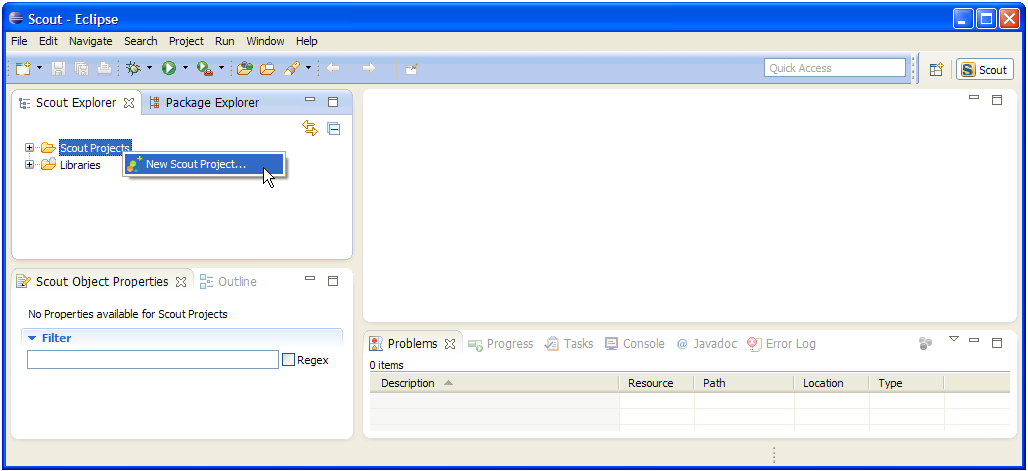
\includegraphics[width=14cm]{sdk_create_new_scout_project.png}
\caption{Create a new Scout project using the Scout SDK perspective.}
\figlabel{sdk_create_new_scout_project}
\end{figure}

In the \wizard{New Scout Project} enter a name for you Scout project. 
As we are creating a ''Hello World'' application, use \java{org.eclipsescout.helloworld} for the \field{Project Name}.
Now, click the \button{Finish} to let the Scout SDK create the initial project code for you.

\begin{figure}
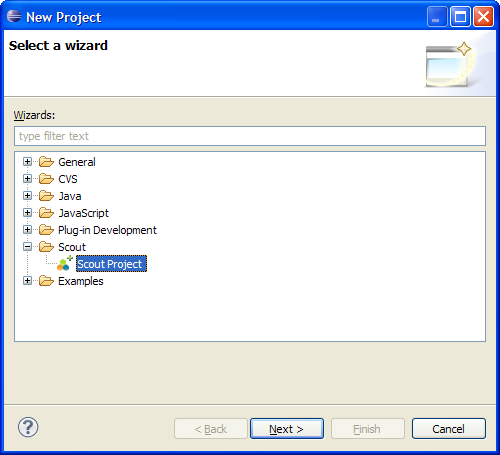
\includegraphics[width=7cm]{sdk_new_project_1.png} \hspace{5mm}
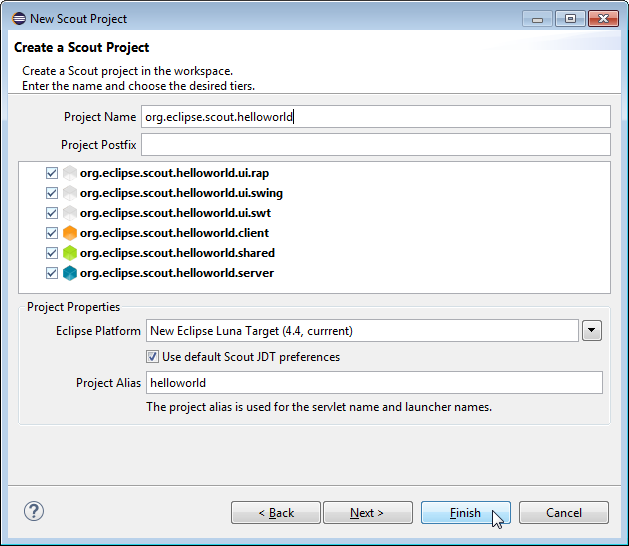
\includegraphics[width=7cm]{sdk_new_project_2.png}
\caption{The new project wizard. The dialog on the left side is only shown when using the generic \wizard{New Project} of Eclipse}
\index{SDK Wizard!New Scout Project}
\figlabel{sdk_new_project_wizard}
\end{figure}

\begin{figure}
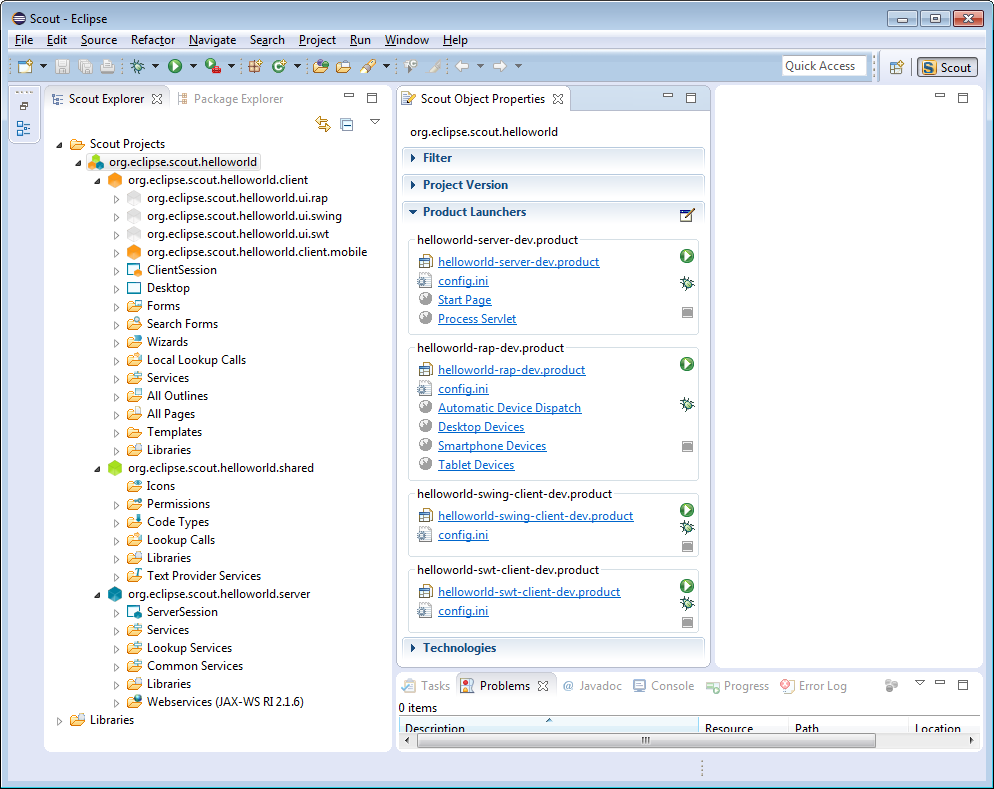
\includegraphics[width=14cm]{sdk_initial_helloworld_project.png}
\caption{The Scout SDK showing the tree representation of our ''Hello World'' application in the Scout Explorer.
Scout Object Properties displays the product launchers for the server and the available clients.}
\figlabel{sdk_initial_helloworld_project}
\end{figure}

Once the initial project code is built, the Scout SDK displays the application model in the \textit{Scout Explorer}.
This model is visually presented as a tree structure covering both the client and the server part of the application.
In \figref{sdk_initial_helloworld_project} the Scout Explorer displays the top level elements of the complete Scout application.

% --------------------------------------------------------------------------- %
\section{Run the Initial Application}
\seclabel{run_initial}

After the initial project creation step we are ready to start the server and the clients of the still empty Scout application.
For this, we switch to the Scout Explorer and select the root node \element{org.eclipse.scout.helloworld}.
Selecting the application's \node{org.eclipse.scout.helloworld} in the Scout Explorer displays the product launchers in the \textit{Scout Object Properties}.
As we can see in \figref{start_client}, we have product launchers for four different development products.

\begin{tabular}{ l l }
  \textbf{RAP}    & The RAP server application for web and mobile clients\\
  \textbf{Swing}  & The Scout Swing desktop client application\\
  \textbf{SWT}    & The Scout SWT desktop client application\\
  \textbf{Server} & The Scout server application\\
\end{tabular}

\begin{figure}
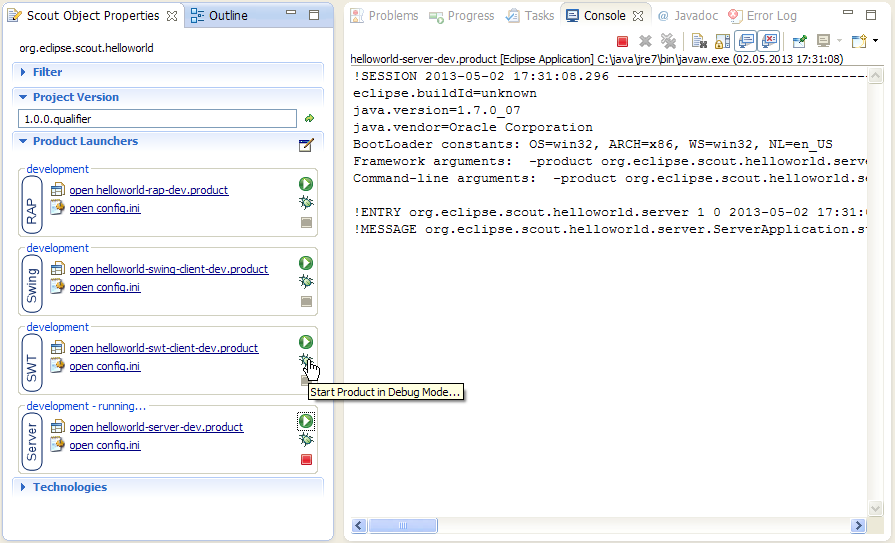
\includegraphics[width=14cm]{sdk_start_client_product.png} 
\caption{Starting the SWT client in the Scout SDK using the provided SWT product launcher. Make sure to start the server before starting any client product.}
\figlabel{start_client}
\index{Product launchers}
\end{figure}

Each product launcher box provides a link to the corresponding Eclipse product file\footnote{
Product files define all the necessary elements of an application.
},
the configuration file\footnote{
The configuration file \filename{config.ini} provides parameters that are read at startup of the corresponding program.
},
as well as three launcher icons to start and stop the corresponding application.
The green \icon{Circle} starts the product in normal mode.
The \icon{Bug} just below, starts a product in debug mode.
To terminate a running product, the red \icon{Square} is provided. 
Alternatively, you can also stop products by clicking on the same red icon in the console view.
This is shown on the right hand side of \figref{start_client}.
Client products may also be stopped by closing the client's main window or using the provided \menu{File|Exit}.

Before any of the client products is started, we need to start the server product using the green circle or the bug launcher icon.
During startup of the Scout server you should see console output similar to the one shown on the right hand side of \figref{start_client}.
Once the server is running, you may start the SWT client as shown in \figref{start_client}, the Swing client, and the RAP server in the same way.
With a running RAP product, you may also display the Scout client in a web browser.
Just type the address \texttt{http://localhost:8082/web} into the browser's navigation bar.

\begin{figure}
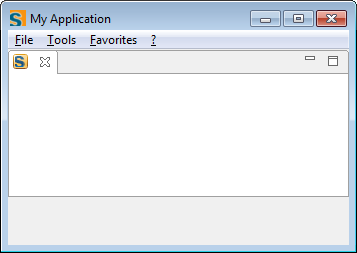
\includegraphics[width=4.5cm]{hellworld_empty_swing.png} \hspace{3mm}
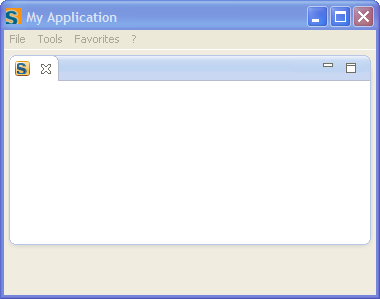
\includegraphics[width=4.5cm]{hellworld_empty_swt.png} \hspace{3mm}
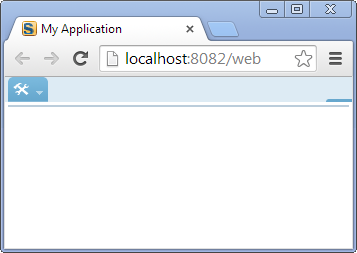
\includegraphics[width=4.5cm]{hellworld_empty_rap.png}
\caption{Running the three client applications. 
Each client displays an empty desktop form. 
From left to right: The Swing client, the SWT client, and the web client}
\figlabel{helloworld_empty}
\end{figure}

Having started the Scout server and all client products, the client applications should become visible as shown in \figref{helloworld_empty}.

% --------------------------------------------------------------------------- %
\section{The User Interface Part}
\seclabel{helloworld_ui}

In this section we will define the user interface (UI) model for the ''Hello World'' application.
More specifically, we add a text field widget to the client's empty desktop form of the ''Hello World'' application.
In the steps described below, we use the \wizard{New Form Field} provided by the Scout SDK. 
First, we add a group box field to the desktop form.
Then, we apply this wizard a second time to add the actual text widget\footnote{
Adding top level group boxes to a form helps in structuring the form layout, especially when a form contains a large number of form fields.
}.

\begin{figure}
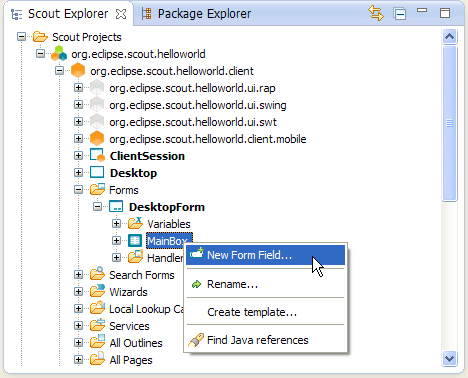
\includegraphics[width=8cm]{sdk_new_field_wizard_menu.png} 
\caption{Using the \menu{New Form Field ...} to start the form field wizard provided by the Scout SDK.}
\figlabel{new_field_context_menu}
\end{figure}

To add any widgets to the desktop form we first need to navigate to the \element{DesktopForm} in the Scout Explorer.
By clicking on the small plus icon on the left hand side of the \element{DesktopForm} this element is expanded and the \element{MainBox} element becomes visible below.
With a click of the right mouse button over the \element{MainBox}, the available context menus are displayed.
To start the form field wizard we select the \menu{New Form Field ...} as shown in \figref{new_field_context_menu}.

\begin{figure}
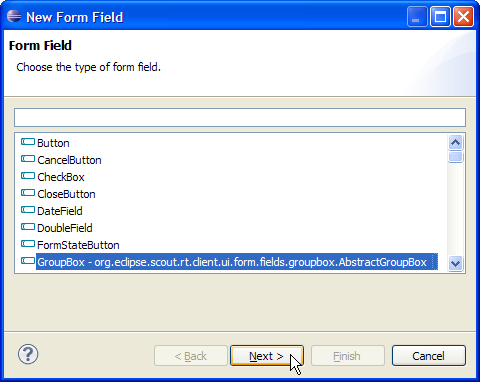
\includegraphics[width=7cm]{sdk_new_field_groupbox_1.png} \hspace{8mm}
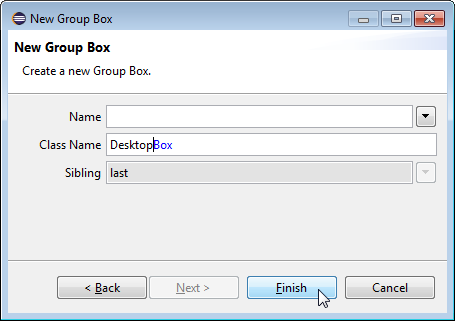
\includegraphics[width=7cm]{sdk_new_field_groupbox_2.png}
\caption{Adding the \textit{DesktopBox} field with the Scout SDK form field wizard.}
\index{SDK Wizard!New Form Field}
\figlabel{helloworld_groupboxfield}
\end{figure}

In the first dialog of the form field wizard shown on the left side of \figref{helloworld_groupboxfield}, we choose the form field type.
To select the desired field type, we either select the desired type with the mouse or use the search field to filter the list of available field types.
In the second wizard dialog, we do not provide a label for the group box in the \field{Name}.
As we have only a single group box in the ''Hello World'' desktop form we omit the name and enter 'Desktop' into the \field{Class Name} before we close the wizard with the \button{Finish}.
This step is shown on the right side of \figref{helloworld_groupboxfield}.
The Scout SDK will add the necessary Java code for the \java{DesktopBox} in the background.

\begin{figure}
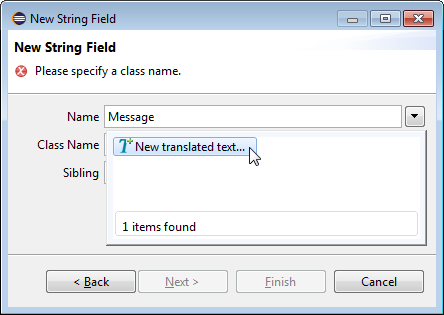
\includegraphics[width=6cm]{sdk_new_field_stringfield_1.png} \hspace{8mm}
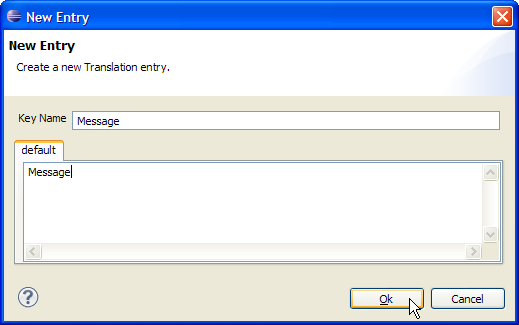
\includegraphics[width=7cm]{sdk_new_field_stringfield_2.png}
\caption{Adding a \textit{StringField} and providing a new translation entry.}
\index{SDK Wizard!Add Translation Entry}
\figlabel{helloworld_stringfield}
\end{figure}

To add the text field widget to the group box just created, we navigate to the corresponding \element{DesktopBox} in the Scout Explorer.
For this, we click on the small plus icon on the left hand side of the \element{MainBox} to expand this node and make the \element{DesktopBox} element visible.
On \element{DesktopBox} we again use the \menu{New Form Field ...}.
In the first wizard dialog, we select \element{StringField} using 'st' as a search criteria and click the \button{Next} to open the second wizard dialog.
In the second wizard dialog, we enter 'Message' into the \field{Name}.
As we do not yet have the text 'Message' available in our ''Hello World'' application the wizard prompts the user with the proposal \textsc{New Translated Text ...}.
Selecting the provided option we can add a new text entry as shown in \figref{helloworld_stringfield}.
Once we have provided some initial translation for our message label, we can close the translation dialog with the \button{Ok}.
Finally, we close the form field wizard using the \button{Finish}.

\begin{figure}
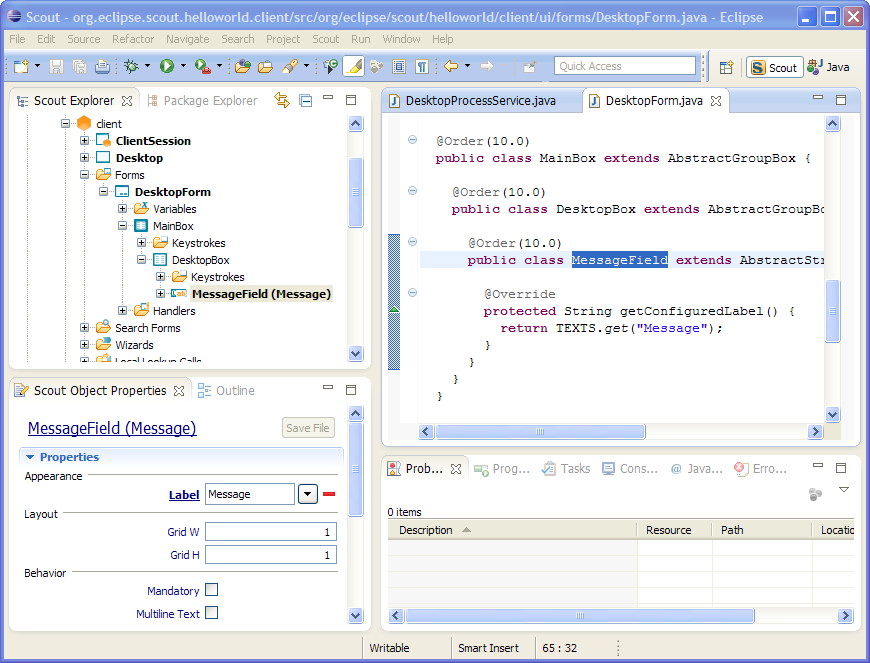
\includegraphics[width=14cm]{sdk_helloworld_messagefield.png}
\caption{Scout SDK showing the \it{MessageField}}
\figlabel{helloworld_messagefield}
\end{figure}

By expanding the \element{DesktopBox} element in the Scout Explorer, the new message field becomes visible. 
A double click on the message field element then loads the corresponding Java code into an Editor as shown in \figref{helloworld_messagefield}.
If you are following this tutorial with your own Eclipse Scout installation compare your status with this screenshot.
Make sure that the project structure in the Scout Explorer looks as shown in \figref{helloworld_messagefield} and a double click to the \element{MessageField} both loads the corresponding Java code and displays the message field's properties in the Scout Object Properties.

Having verified your status of the ''Hello World'' application you can start the application as described in \secref{run_initial}.
The client applications will then display your message widget.
However, the text widget is still empty, as we did not yet load any initial content into it.
This is the topic of the next section where we continue the tutorial with the server part.

% --------------------------------------------------------------------------- %
\section{The Server Part}
\seclabel{helloworld.server}

The responsibility of the server part in our ''Hello World'' application is to provide an initial text content for the message field in the client's user interface.
We implement this behaviour in the \java{load} method of the server's \java{DesktopService}.
An empty stub for the \java{load} method and the \java{DesktopService} service have already been created during the initial project creation step described in \secref{create_project_simple}.
The \java{DesktopService} represents the server service corresponding to the \java{DesktopForm} on the client side.
This initial setup represents Scout's standard form processing mechanism where client forms and server services typically come in pairs.

Whenever the client's user interface displays a form to the user, the client connects to the server and calls the \java{load} method of the corresponding server service.
We can now add the business logic to the \java{load} method of the server's \java{DesktopService} to implement the desired behaviour.
And this is the last missing piece to complete the ''Hello World'' application.

\begin{figure}
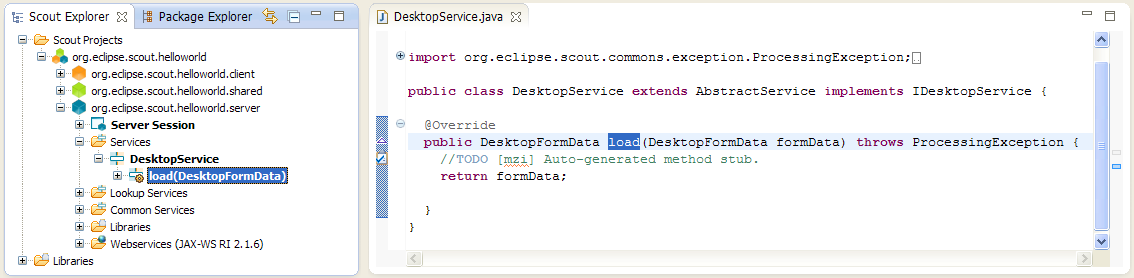
\includegraphics[width=14cm]{sdk_server_desktopservice_load.png}
\caption{The Scout Explorer showing the blue server node expanded with the \folder{Services}.
In this folder the \element{load} method of \element{DesktopService} is selected and its initial implementation is shown in the editor on the right side.}
\figlabel{helloworld_load_servicemethod}
\end{figure}

To navigate to the implementation of the desktop service in the Scout SDK, we first expand the blue top-level \node{server} in the Scout Explorer.
Below the server node, we then expand the \folder{Services} which shows the \element{DesktopService} element.
Expanding this \element{DesktopService} node, the \java{load} method becomes visible as shown in \figref{helloworld_load_servicemethod}.

\begin{lstlisting}[backgroundcolor=\color{white}]
  @Override
  public DesktopFormData load(DesktopFormData formData) throws ProcessingException {
    //TODO [mzi] Auto-generated method stub.
    return formData;
  }
\end{lstlisting}
  
According to the signature of the \java{load} method, a \java{formData} object is passed into this method that is then handed back in the return statement.
To complete the implementation of the \java{load} method it is sufficient to assign the text 'hello world!' to the message field part of the form data.
The only line of Java code we write in our ''Hello World'' application is printed below.
For the complete implementation of the load method see \lstref{helloworld.load}.

\begin{lstlisting}[backgroundcolor=\color{white}]
  formData.getMessage().setValue("hello world!");
\end{lstlisting}

\lstinputlisting[
  label=\lstlabel{helloworld.load},
  caption=Assigning "hello world" to the form data's message field.,
  index={DesktopFormData,DesktopProcessService},
  linerange={10-15},
  float
]
{../code/helloworld/org.eclipse.scout.helloworld.server/src/org/eclipse/scout/helloworld/server/services/DesktopService.java}

% --------------------------------------------------------------------------- %
\section{Add the Rayo Look and Feel}

\begin{figure}
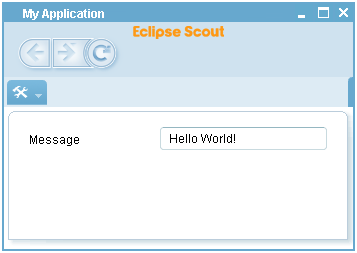
\includegraphics[width=7cm]{helloworld_message_swing_rayo.png} \hspace{5mm}
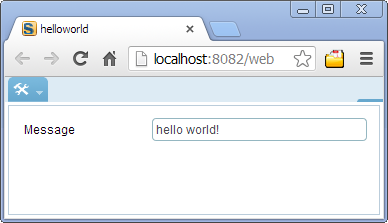
\includegraphics[width=7cm]{helloworld_message_rap_rayo.png}
\caption{The ''Hello World'' client application with the Rayo look and feel. The desktop client is shown on the left and the web client on the right hand side.}
\figlabel{helloworld_clientapp}
\end{figure}

For Eclipse Scout applications a slick look and feel called Rayo is available in the Eclipse Marketplace\footnote{
Eclipse Marketplace: \url{http://marketplace.eclipse.org/}
}.
And in this (optional) part of the ''Hello World'' tutorial we will add Rayo to our ''Hello World'' Swing client application.
As a result, we will get a Scout desktop application that looks the same as the corresponding Scout web client as shown in \figref{helloworld_clientapp}.

\begin{figure}
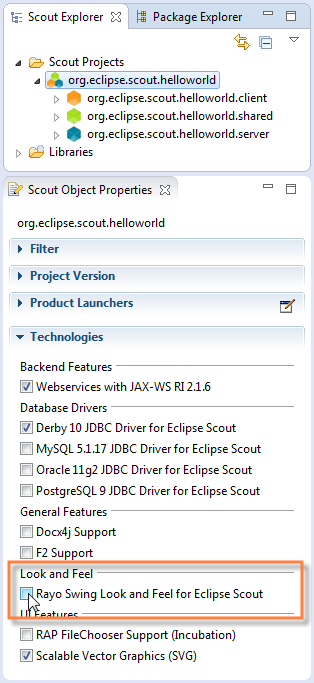
\includegraphics[width=6cm]{sdk_rayo_add_checkbox.png} \hspace{5mm}
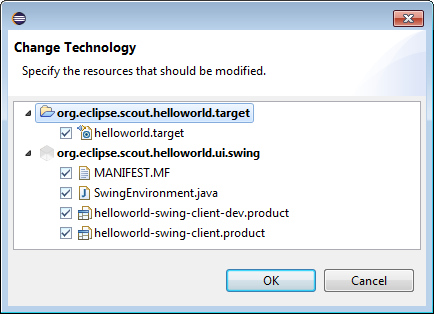
\includegraphics[width=7cm]{sdk_rayo_confirm_changes.png}
\caption{Adding the Rayo Swing look and feel. The Rayo checkbox to activate the look and feel is highlighted on the left hand side. The dialog on the right hand side shows the changes in the Swing plugin that will be made by the Scout SDK.}
\figlabel{selecting_rayo}
\end{figure}

To add Rayo in the Scout SDK to our ''Hello World'' project, switch to the Scout Explorer and select the top-level \node{org.eclipse.scout.helloworld}.
Then, according to \figref{selecting_rayo}, select the checkbox \element{Rayo Swing Look and Feel for Eclipse Scout} under the \element{Technologies} section of the Scout Object Properties.
This brings up a dialog showing the proposed changes to the Swing plugin of the ''Hello World'' application. 
These changes need to be confirmed with the \button{OK}.
The first time the user adds the Rayo feature in the Scout SDK, Eclipse needs to download the package from the Eclipse Marketplace.
This download and subsequent installation of Rayo will make you to go through the following steps.

\begin{enumerate}
  \item Accept Licence: GPL with Classpath Exception
  \item Accept unsigned content
  \item Restart the Eclipse IDE
\end{enumerate}

After the successful download and installation of the Rayo package, start the Swing client using the procedure described in \secref{run_initial}.
When we also start the web client of the ''Hello World'' application using the RAP product launcher, we can compare the result side by side.

% --------------------------------------------------------------------------- %
\section{Exporting the Application}
\seclabel{helloworld_export}

We are now ready to move the finished ''Hello World'' application from our development environment to a productive setup.
The simplest option to move our application into the 'wild' is to use the \wizard{Export Scout Project} provided by the Scout SDK.
Using the default settings, the export wizard produces two WAR files\footnote{
Web application ARchive (WAR): \url{http://en.wikipedia.org/wiki/WAR_file_format_(Sun)}
}
that contain the complete Scout server and the desktop and mobile client applications.

To deploy the application to a web server the WAR files generated by the wizard are the only artefacts needed.
The first WAR file contains the Scout server including a zipped desktop client for downloading.
In the second WAR file, the RAP server application that provides both the web client and the client for mobile devices.

\begin{figure}
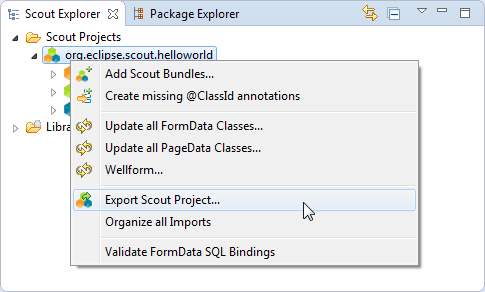
\includegraphics[width=8cm]{sdk_export_war_menu.png} 
\caption{Starting the \wizard{Export Scout Project} in the Scout SDK with the context menu. 
In the first wizard step, the target directory for the WAR files and the artefacts to export are specified.}
\index{SDK Wizard!Export Scout Project}
\figlabel{sdk_export_war}
\end{figure}

\begin{figure}
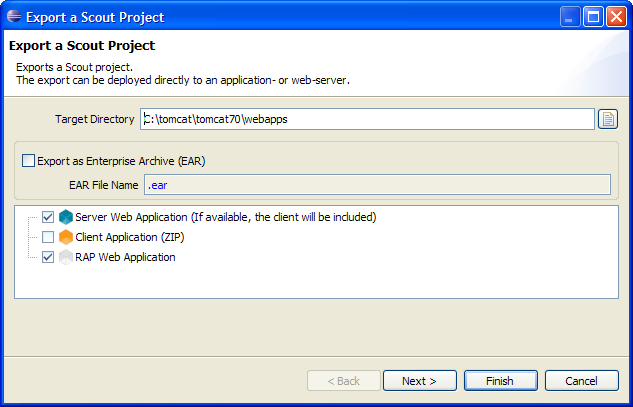
\includegraphics[width=10cm]{export_wizard_1.png}
\caption{The first dialog of the \wizard{Export Scout Project}. 
Here, the target directory for the WAR files that will be generated by the wizard is specified.}
\figlabel{export_wizard_1}
\end{figure}

To start the export wizard, we the Scout SDK started with the ''Hello World'' Scout project.
In the Scout Explorer we then select the corresponding \contextmenu{Export Scout Project...} on the ''Hello World'' top level application node as shown in \figref{sdk_export_war}.
In the first wizard dialog shown in \figref{export_wizard_1}, the target directory for the WAR files needs to be specified.
You may choose any directory as the target directory\footnote{
Make sure to remember the location of this directory.
We will need the directory location again when we deploy these WAR files to the Tomcat web server.
}.
After clicking \button{Next} the second wizard step proposes the server product file that specifies the artefacts to be exported including the file name for the WAR file for the ''Hello World'' server application.
Typically, the proposed default values are fine.
Move to the third dialog with \button{Next}.

\begin{figure}
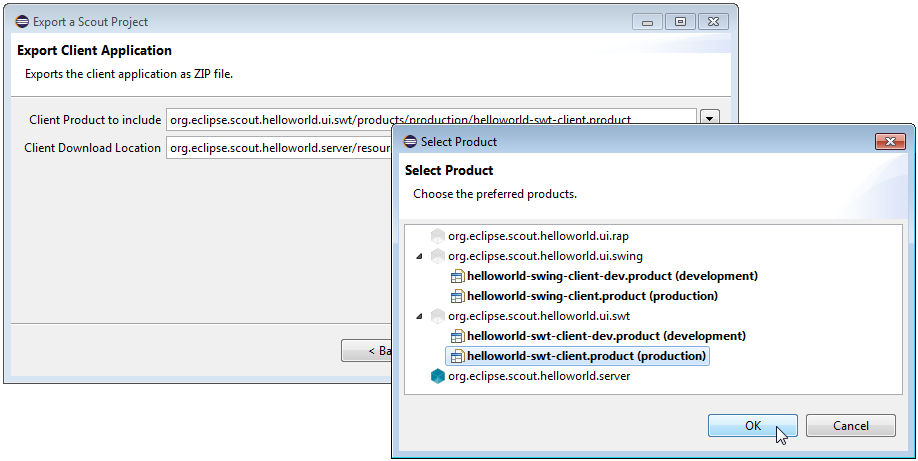
\includegraphics[width=13cm]{export_wizard_3.png}
\caption{The third dialog of the \wizard{Export Scout Project} defines the client application to be included in the \texttt{helloworld\_server.war} file.
In the last step of the export wizard the RAP sever is exported to the specified file name (right).}
\figlabel{export_wizard_3}
\end{figure}

In the third dialog of the \wizard{Export Scout Project} the desktop client to be included in the WAR file needs to be specified.
The default selection is set to the SWT client application.
For the ''Hello World'' example, we want to include the Swing client application with the Rayo Look and Feel.
For this, we need to change the selected product to \element{helloworld-swing-client.product (production)} according to \figref{export_wizard_3}.
With \button{Next} we move to the last wizard step.

\begin{figure}
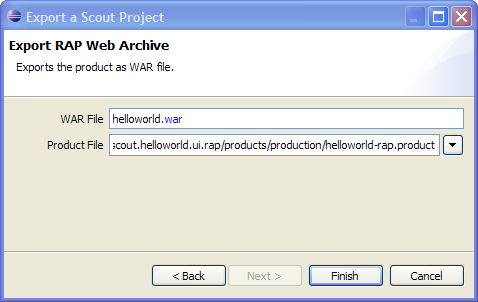
\includegraphics[width=8cm]{export_wizard_4.png}
\caption{The last dialog of the \wizard{Export Scout Project} defines the export of the RAP server.
Normally, the proposed field values do not need any adjustments.}
\figlabel{export_wizard_4}
\end{figure}

In the last wizard dialog shown in \figref{export_wizard_4}, the RAP server product and the corresponding WAR file name are specified.
Normally, the proposed field values are fine and we can close the wizard with \button{Finish}.
After this last step, the Scout SDK is assembling the necessary artefacts and building the two ''Hello World'' WAR files.
These two WAR files are the only items needed for deploying the ''Hello World'' application to a web server

% --------------------------------------------------------------------------- %
\section{Deploying to Tomcat}
\seclabel{helloworld_deploy}

As the final step of this tutorial, we deploy the two WAR files representing our ''Hello World'' application to a Tomcat web server.
For this, we first need a working Tomcat installation.
If you do not yet have such an installation you may want to read and follow the instructions provided in \appref{install_tomcat}.
To verify a running Tomcat instance, type \url{http://localhost:8080/} into the address bar of the web browser of your choice.
You should then see the page shown in \figref{deploy_tomcat_1}.

\begin{figure}
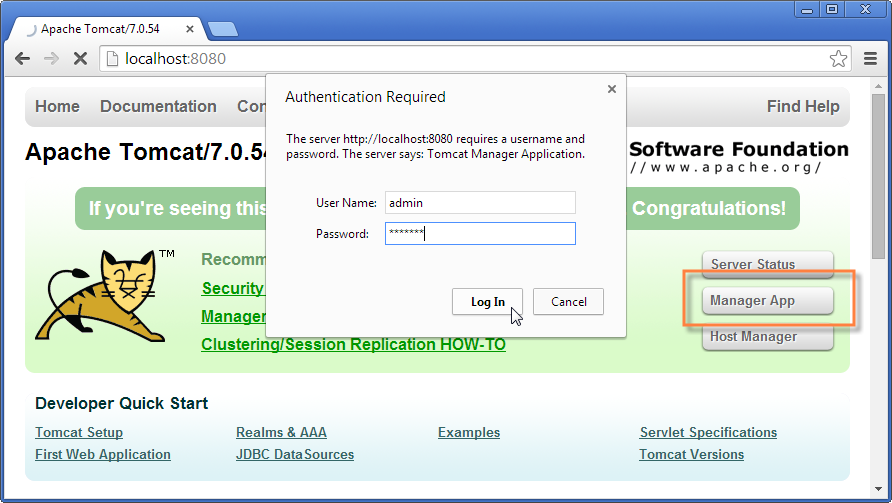
\includegraphics[width=14cm]{tomcat_managerapp_login.png} 
\caption{The Tomcat shown after a successful installation. 
After clicking on the ''Manager App'' button (highlighted in red) the login box is shown in front.
A successful login shows the ''Tomcat Web Application Manager''.}
\figlabel{deploy_tomcat_1}
\end{figure}

\begin{figure}
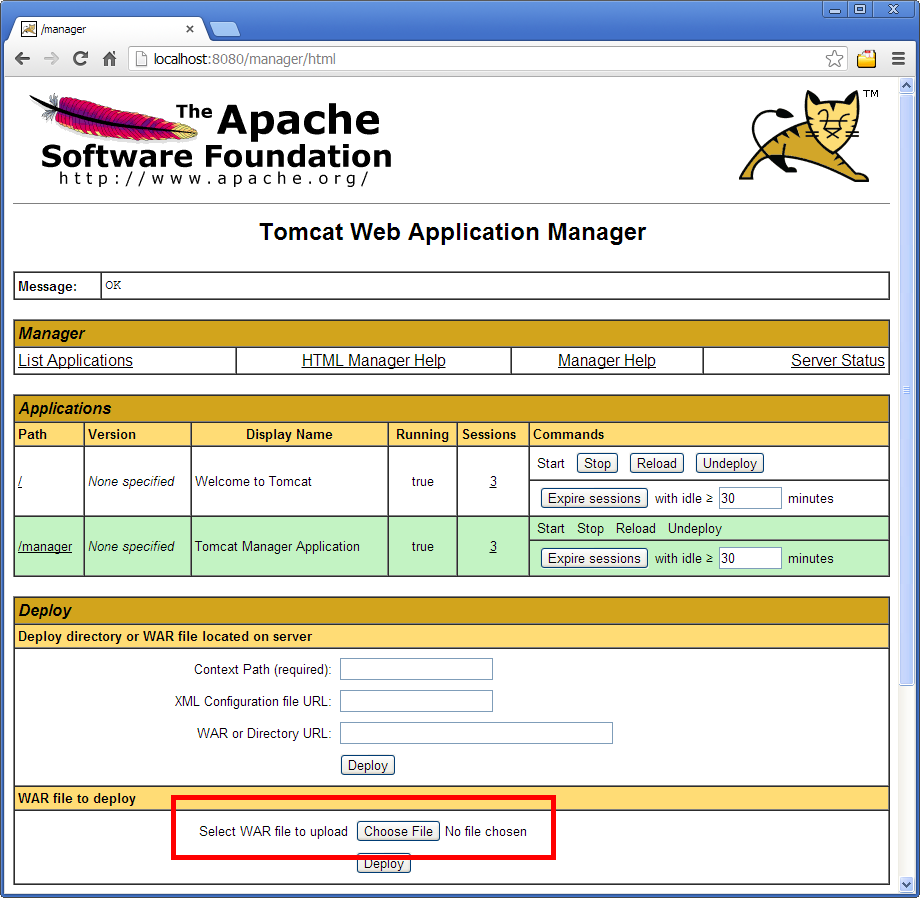
\includegraphics[width=14cm]{tomcat_managerapp_selectwar.png}
\caption{The ''Tomcat Web Application Manager''.
The WAR files to be deployed can then be selected using button ''Choose File'' highlighted in red.}
\figlabel{deploy_tomcat_2}
\end{figure}

Once the web browser displays the successful running of your Tomcat instance, switch to its ''Manager App'' by clicking on the button highlighted in \figref{deploy_tomcat_1}.
After entering user name and password the browser will display the ''Tomcat Web Application Manager'' as shown in \figref{deploy_tomcat_2}.
If you don't know the correct username or password you may look it up in the file \filename{tomcat-users.xml} as described in \appref{tomcat_dirs_and_files}.

After logging successfully into Tomcats manager application, you can select the WAR file(s) to be deployed using button ''Choose File'' according to the right hand side of \figref{deploy_tomcat_2}.
After picking your \filename{helloworld_server.war} and \filename{helloworld.war} file and closing the file chooser, click on button ''Deploy'' (located below button ''Choose File'') to deploy the application to the Tomcat web server.
This will copy the selected WAR file into Tomcats \filename{webapps} directory and unpack its content into a subdirectory with the same name.
Deploying the file \filename{helloworld.war} will extract its contents into a subdirectory named \filename{helloworld} as shown in \figref{tomcat.install.dir}.
Accordingly, the file \filename{helloworld_server.war} will be extracted into subdirectory \filename{helloworld_server}.
You can now connect to the deployed application using the browser of your choice and enter the following address.

\begin{lstlisting}
  http://localhost:8080/helloworld_server/
\end{lstlisting}

\begin{figure}
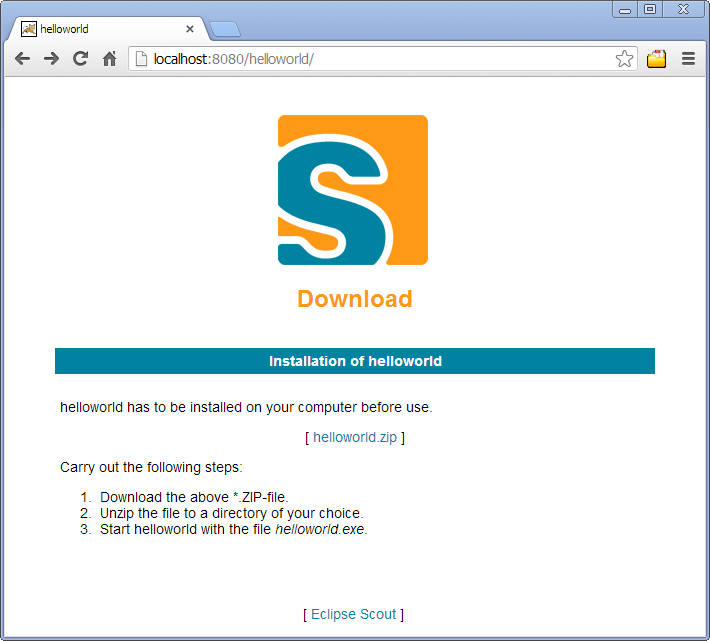
\includegraphics[width=12cm]{tomcat_helloworld_download.png}
\caption{The ''Hello World'' home page, providing a link to download the desktop client.}
\figlabel{helloworld_running_download}
\end{figure}

You will then see the home page of the server of your ''Hello World'' application shown in \figref{helloworld_running_download}.
From here you can download the zipped client application that can be saved in a directory of your choice.
After unpacking the zip file, you may start the executable file named \filename{helloworld}.
This will start the ''Hello World'' client application as shown on the left hand side of \figref{helloworld_running_clients}.
To start the ''Hello World'' web application, open a browser and enter the following address.

\begin{lstlisting}
  http://localhost:8080/helloworld/
\end{lstlisting}

\begin{figure}
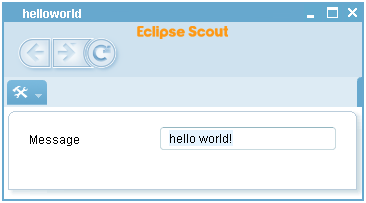
\includegraphics[height=2.5cm]{helloworld_finished_rayo_swing.png}\hspace{5mm}
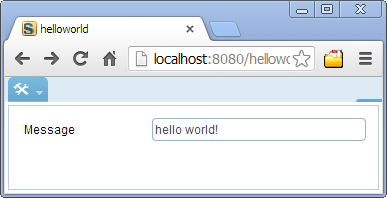
\includegraphics[height=2.5cm]{helloworld_finished_rayo_rap.png}\hspace{5mm}
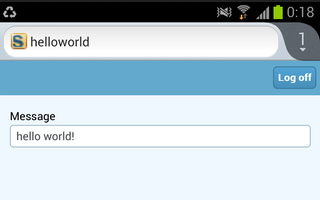
\includegraphics[height=2.5cm]{helloworld_finished_rayo_rap_mobile.png}
\caption{The ''Hello World'' client application running on the desktop, in the browser and on a mobile device.}
\figlabel{helloworld_running_clients}
\end{figure}

Depending on the device your browser is running on you will be redirected to \texttt{helloworld/web} on a desktop or laptop computer, to \texttt{helloworld/mobile} on a mobile device or to \texttt{helloworld/mobile} if you are connecting from a tablet device.
\figref{helloworld_running_clients} shows screenshots for a desktop client, the web application and the same application in a mobile browser.
As demonstrated in these screenshots \texttt{helloworld/web} and \texttt{helloworld/mobile} lead to a different presentation of the same UI optimized to the target form factors of desktop browsers, tablets, and mobile phones.

% =========================================================================== %
\chapter{''Hello World'' Background}
\chalabel{helloworld_background}

The previous ''Hello World'' tutorial has been designed to cover the creation of a complete client server application in a minimal amount of time.
In this chapter, we will take a deeper look at the ''Hello World'' and provide background information along the way.
The goal is to explain many of the used concepts in the context of a concrete Scout application to allow for a well rounded first impression of the Eclipse Scout framework and the tooling provided by the Scout SDK.

The structure of this chapter is closely related to the ''Hello World'' tutorial.
As you will notice, the order of the material presented here exactly follows the previous tutorial and identical section titles are used where applicable.
In addition to \charef{helloworld}, we include \secref{initial_helloworld} to discuss the initial application generated by the Scout SDK.

% --------------------------------------------------------------------------- %
\section{Create a new Project}
\seclabel{create_project_simple_background}

The first thing you need for the creation of a new Scout project is to select a new workspace.
For Eclipse, a workspace is a directory where Eclipse can store a set of projects in a single place.
As Scout projects typically consist of several Eclipse plugin projects the default (and recommended) setting is to use a single workspace for a single Scout project.

\begin{figure}
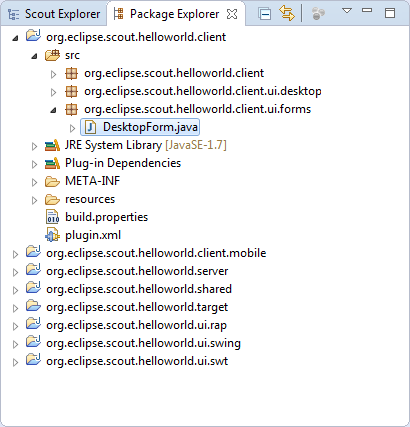
\includegraphics[width=7cm]{sdk_package_explorer.png} \hspace{0.5cm}
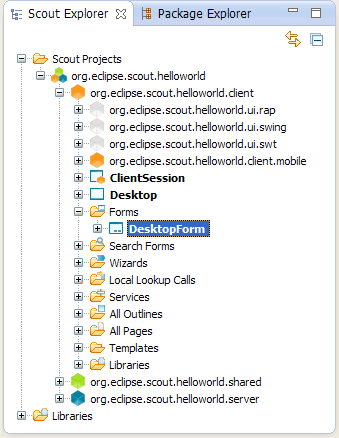
\includegraphics[width=7cm]{sdk_scout_explorer.png}
\caption{The Eclipse plugin projects of the ''Hello World'' application shown by the Package Explorer in the Scout SDK on the left hand side. 
The corresponding view in the Scout Explorer is provided on the right hand side.
}
\figlabel{package_explorer}
\end{figure}

In the case of the ''Hello World'' application, the workspace contains seven plugin projects as shown on the left side of \figref{package_explorer}.
In the expanded source folder of the client plugin \element{org.eclipse.scout.helloworld.client} the organisation of the Java packages is revealed.
The Scout Explorer provided on the right side of \figref{package_explorer} shows three colored top level nodes below the main project \element{org.eclipse.scout.helloworld}.

In the Scout Explorer, the main project node expands to the orange client node \element{org.eclipse.scout.helloworld.client}, the green shared node \element{org.eclipse.scout.helloworld.client} and the blue server node \element{org.eclipse.scout.helloworld.server}.
The client node first presents the white user interface (UI) nodes \element{org.eclipse.scout.helloworld.client.ui.*} indicating the supported UI technologies.
Next, the client mobile node \element{org.eclipse.scout.helloworld.client.mobile} is shown.
It is responsible for adapting the layout of the user interface suitably for mobile and tablet devices.
Finally, after the \node{ClientSession} and the \node{Desktop}, component specific folders allow for a simple navigation to the various client parts.

Comparing the Package Explorer with the Scout Explorer a couple of aspects are notable.
First, the number and names of the Eclipse plugin projects is identical in both the Package Explorer and the Scout Explorer view.
However, the Scout Explorer recognizes the Scout project structure and explicitly renders the relation between the different Eclipse plugins.
In addition, individual node colors are used to indicate the role of each plugin project.
Second, the focus of the Scout Explorer lies on the business functionality of the complete client server application.
Artefacts only necessary to the underlying Eclipse platform are not even accessible.
Third, on the individual elements rendered in the Scout Explorer, the Scout SDK provides menus to start wizards useful to the selected context.
In the case of the ''Hello World'' tutorial we could create the complete application (except for a single line of Java code) using these wizards .

When we revisit the \wizard{New Scout Project} in \figref{sdk_new_project_wizard}, it now becomes trivial to explain how the \field{Project Name} \java{org.eclipse.scout.helloworld} was used as the common prefix for plugin project names and Java package names.
Based on the project name, the last part \java{helloworld} was used for the \field{Project Alias}.
As we have seen in \secref{helloworld_export}, this project alias is used by the Scout SDK to build the base names of the WAR files in the export step.
In turn, after deploying the WAR files as described in \secref{helloworld_deploy}, the RAP server application becomes available under the URL \java{http://localhost:8080/helloworld}.
Should you have a catchy naming for you application in mind, \java{com.mycompany.mycatchyname} is therefore a good choice for the \field{Project Name}.


% --------------------------------------------------------------------------- %
\section{Walking through the Initial Application}
\seclabel{initial_helloworld}

In this section, we will walk you through the central Scout application model components of the ''Hello World'' example. 
As each of these components is represented by a Java class in the Scout framework, we can explain the basic concept using the available ''Hello World'' source code.
Below, we will introduce the following Scout components.

\begin{itemize}
  \item Desktop
  \item Form
  \item Form handler
  \item Service
  \item MainBox
  \item Form data
  \item Form field
\end{itemize}

Please note that most of the Java code was initially generated by Scout SDK.
In many cases this code can be used ''as is'' and does not need to be changed.
Depending on your requirements, it might very well be that you want to adapt the provided code to fit your specific needs.
However, a basic understanding of the most important Scout components should help you to better understand the structure and working of Scout applications.

% ........................................................................... %
\subsection{Desktop}

The desktop is the central container of all visible elements of the Scout client application.
It inherits from Scout class \java{AbstractDesktop} and represents the empty application frame with attached elements, such as the applications menu tree.
In the ''Hello World'' application, it is the Desktop that is first opened when the user starts the client application.

To find the desktop class in the Scout Explorer, we first navigate to the orange \node{client} and double click the \node{Desktop} just below.
This will open the associated Java file \texttt{Desktop.java} in the editor view of the Scout SDK.
Of interest is the overwritten callback method \java{execOpened} shown in \lstref{helloworld.execopened}.

\lstinputlisting[
  label=\lstlabel{helloworld.execopened},
  caption=Creating and starting a form in the client's Desktop callback method \java{execOpened}.,
  index={DesktopForm},
  linerange={32-41},
  float
]
{../code/helloworld/org.eclipse.scout.helloworld.client/src/org/eclipse/scout/helloworld/client/ui/desktop/Desktop.java}

Method \java{execOpened} is called by the Scout framework after the desktop frame becomes visible.
The only thing that happens here is the creation of a \java{desktopForm} object, that gets assigned an icon before it is started via method \java{startView}.
This desktop form object holds the \field{Message} text widget that is displayed to the user\footnote{
In the Scout application model we can only add UI fields to Scout form elements, not directly to the desktop.
}.
More information regarding form elements are provided in the next section.

% ........................................................................... %
\subsection{Form}
\seclabel{helloworld.form}

Scout forms are UI containers that hold form field widgets.
A Scout form always inherits from Scout class \java{AbstractForm} and can either be displayed as a dialog in its own window or shown as a view inside of another UI container.
In the ''Hello World'' application a \java{DesktopForm} object is created and displayed as a view inside of the desktop element.

To find the desktop form class in the Scout Explorer, expand the orange \node{client}\footnote{
To expand elements (nodes, folders, etc.) in the Scout Explorer, use a double click on the element or a single click on the plus icon in front of the element.}.
Below this node, you will find the \folder{Forms}. 
Expand this folder to show the \element{DesktopForm} as shown in \figref{helloworld_viewhandler}.
In the Scout Object Property window in the screenshot, we can also see the \property{Display Hint}.
Its value is set to 'View' to display the desktop form as a view and not as a dialog in its own frame.

\begin{figure}
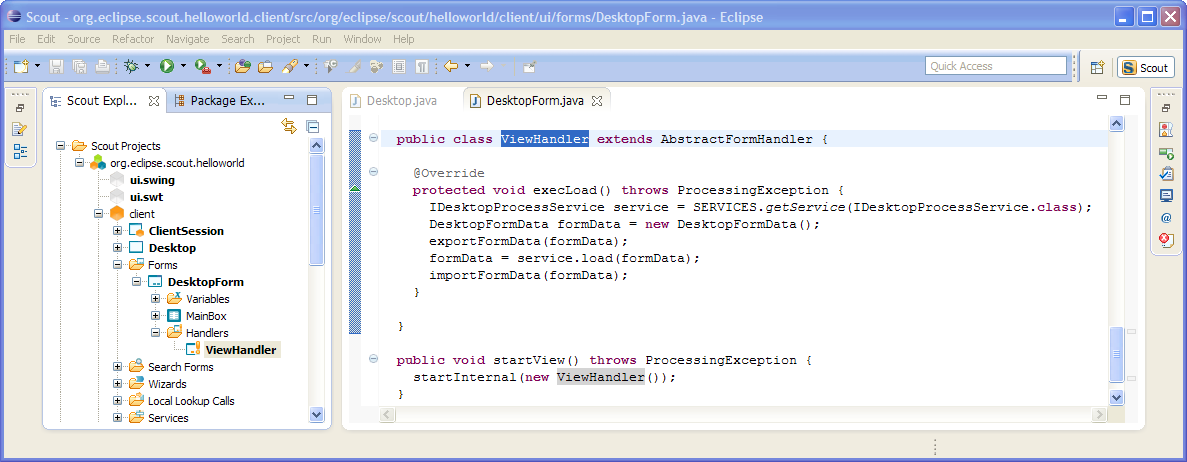
\includegraphics[width=15cm]{sdk_helloworld_viewhandler.png}
\caption{Scout SDK showing the DesktopForm's \textit{ViewHandler} in the Scout Explorer and the form properties in the Scout Object Properties.}
\figlabel{helloworld_viewhandler}
\end{figure}

Expand the \element{DesktopForm} to show its children: \element{Variables}, \element{MainBox} and \element{Handlers}.
The \element{Variables} sub folder contains variables. They are invisible to the application user.
The ''Hello World'' application is so simple, it does not need variables.
The sub folder \element{MainBox} contains form fields. These are the visible user interface elements.
The main box of our \java{DesktopForm} holds the \java{DesktopBox} containing the \java{MessageField} added with the \wizard{New Form Field}.
Finally, the \element{Handlers} sub folder contains all available form handlers.
The view handler shown in \figref{helloworld_viewhandler} has been added in the initial project creation step.

% ........................................................................... %
\subsection{Form Handler}
\seclabel{helloworld.formhandler}

Form handlers are used to manage the form's life cycle.
Scout form handlers inherit from \java{AbstractFormHandler} and allow the implementation of desired behaviour before a form is opened, or after it is closed.
This is achieved by overwriting callback methods defined in \java{AbstractFormHandler}.
The necessary wiring is provided by the Scout framework, either by the initial project creation step or when using one of the provided Scout SDK wizards.

\lstinputlisting[
  label=\lstlabel{helloworld.viewhandler},
  caption=Class \java{DesktopForm} with its view handler and \java{startView} method. Other inner classes and methods are omitted here.,
  index={ViewHandler},
  emph={load},
  linerange={20-21,74-91},
  float
]
{../code/helloworld/org.eclipse.scout.helloworld.client/src/org/eclipse/scout/helloworld/client/ui/forms/DesktopForm.java}

In the ''Hello World'' application, it is the overwritten \java{execLoad} method in the \java{ViewHandler} that defines what will happen before the desktop form is shown to the user.
The corresponding source code is provided in \lstref{helloworld.viewhandler}.
It is this \java{execLoad} method where most of the behaviour relevant to the ''Hello World'' application is implemented.
Roughly, this implementation is performing the following steps.

\begin{enumerate}
  \item Get a reference to the forms server service running on the server.
  \item Create a data transfer object (DTO)\footnote{
Data Transfer Object (DTO): \url{http://en.wikipedia.org/wiki/Data_transfer_object}.}
  \item Pass the empty DTO to the load service method (ask the server for some data).
  \item Update the DTO with the content provided by the service load method.
  \item Copy the updated information from the DTO into the desired form field.
\end{enumerate}

To open the \java{ViewHandler} class in the Java editor of the Scout SDK, double click on the \element{ViewHandler} in the Scout Explorer.
Your Scout SDK should then be in a state similar to \figref{helloworld_viewhandler}.
In the lower part of \lstref{helloworld.viewhandler} we can see the wiring between the desktop form and the view handler in method \java{startView}.
Further up, we find method \java{execLoad} of the view handler class.

Before we discuss this method's implementation, let us examine when and how \java{execLoad} is actually called.
As we have seen in the \java{Desktop} class (see \lstref{helloworld.execopened}), the form's method \java{startView} is executed after the desktop form is created.
Inside method \java{startView} (see \lstref{helloworld.viewhandler}), the desktop form is started/opened using \java{startInternal}.
In method \java{startInternal} a view handler is then created and passed as a parameter.
This eventually leads to the call of our \java{execLoad} custom implementation.

We are now ready to dive into the implementation of method \java{execLoad} of the desktop form's view handler.
First, a reference to a form service identified by \java{IDesktopService} is obtained using \java{SERVICES.getService}.
Then, a form data object (the DTO) is created and all current form field values are exported into the form data via method \java{exportFormData}.
Strictly speaking, the \java{exportFormData} is not necessary for the use case of the ''Hello World'' application.
But, as this is generated code, there is no benefit when we manually delete the \java{exportFormData} command.
Next, using the \java{load} service method highlighted in \lstref{helloworld.viewhandler}, new form field values are obtained from the server and assigned to the form data object.
Finally, these new values are imported from the form data into the form via the \java{importFormData} method.
Once the desktop form is ready, showing it to the user is handled by the framework.

To add some background to the implementation of the \java{execLoad} above, the next section introduces services and form data objects. 

% ........................................................................... %
\subsection{Form Services and Form Data Objects}

Form services and form data objects are used in the Scout framework to exchange information between the Scout client and server applications.
When needed, a service implemented on the server side can register a corresponding proxy service on the client.
This proxy service is invoked by the client as if it were implemented locally.
In fact, when we get a service reference using \java{SERVICES.getService}, we do not need to know if this service runs locally on the client or remotely on the server.

In the ''Hello World'' example application, the client's desktop form has an associated desktop service running on the server.
This correspondence between forms and form services is also reflected in the \element{Links} section of the Scout Object Properties of the desktop form.
As shown in \figref{helloworld_viewhandler}, links are provided not only for the desktop form, but for its desktop form data, the corresponding desktop form service as well as for the service interface \java{IDesktopService}. 
On the client, this interface is used to identify and register the proxy service for the desktop service.

To transfer data between the client and the server, the ''Hello World'' application uses a \java{DesktopFormData} object as a DTO.
This form data object holds all form variables and values for all the form fields contained in the form.
Taking advantage of this correspondence, the Scout framework provides the convenience methods \java{exportFormData} and \java{importFormData}.
As a result, the developer does not need to deal with any mapping code between the form data object and the form fields.

The actual implementation of the desktop form service in class \java{DesktopService} is implemented on the server side.
As the class \java{DesktopService} represents an ordinary Scout service it inherits from \java{AbstractService}.
It also implements its corresponding \java{IDesktopService} interface used for registering both the actual service as well as the proxy service.

% --------------------------------------------------------------------------- %
\section{Run the Initial Application}
\seclabel{run_initial_background}

% ........................................................................... %
\subsection{The Launcher Boxes}

To run a Scout application the Scout SDK provides launcher boxes in the Scout Object Properties as described in \secref{run_initial}.
These object properties are associated to the top level project node in the Scout Explorer.
Using the \icon{Edit} provided in the product launcher section of the Scout Object Properties, the list of launcher boxes can be specified as shown in \figref{select_product_launchers}.

\begin{figure}
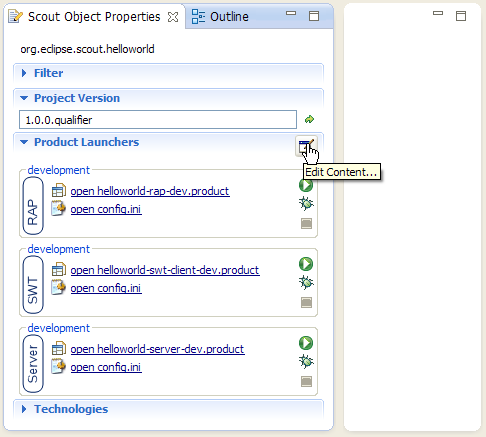
\includegraphics[height=6.5cm]{sdk_edit_product_launcher.png} \hspace{0.5cm}
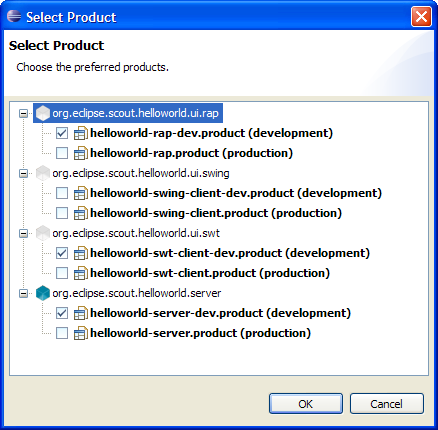
\includegraphics[height=6.5cm]{sdk_select_product_launcher.png}
\caption{Using the \icon{Edit Content...} shown on the left hand side, the product selection dialog shown on the right side is opened.
Using this product selection dialog, the list of launcher boxes can be specified.
}
\figlabel{select_product_launchers}
\end{figure}

% ........................................................................... %
\subsection{Eclipse Product Files}

The available products shown on the right side of \figref{select_product_launchers} represent the Eclipse product files created in the initial project creation step.
Product files\footnote{
Read the following article for an introduction to Eclipse product files: \url{http://www.vogella.com/articles/EclipseProductDeployment/article.html}.
}
are used in Eclipse to specify the configuration and content of an executable application.
In the case of the ''Hello World'' project, four executable applications --- with two Eclipse product files for each application --- have been defined by the Scout SDK.
The four applications, one for the server application and one for each client technology, have already been discussed in \secref{run_initial}.

\begin{figure}
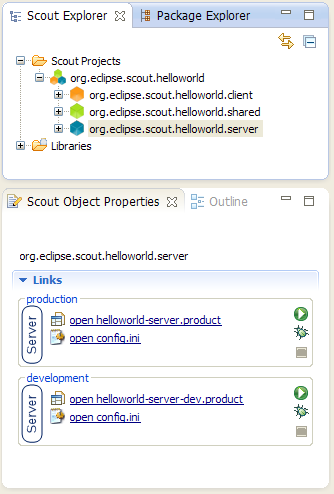
\includegraphics[height=10cm]{sdk_server_node_properties.png} \hspace{0.5cm}
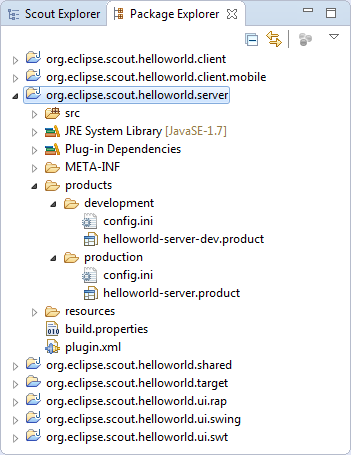
\includegraphics[height=10cm]{sdk_server_plugin_explorer.png}
\caption{The production and development launcher boxes associated with the ''Hello World'' server application are shown on the left side. 
In the Package Explorer shown on the right side, the production and development products are located under the \folder{products} in the server plugin project.
}
\figlabel{server_plugin}
\end{figure}

The reason why each executable has two product files associated with it lies in the assumption that we want to run the Scout application in different environments.
Even in the case of the simple ''Hello World'' example, the Scout application is started in two target environments.
The development environment defines the product in the context of the Scout SDK.
To export and run the Scout application outside of the Scout SDK, the production product files are used to define the application when it is to be started on a Tomcat web server.
\figref{server_plugin} illustrates this situation for the ''Hello World'' server application. 
On the left side, the blue server node is selected in the Scout Explorer.
This opens the two server launcher boxes for the production and the development environment.
On the right side of \figref{server_plugin}, the corresponding plugin project \element{org.eclipse.scout.helloworld.server} is expanded to show the file based organisation of the two product definitions.

\begin{figure}
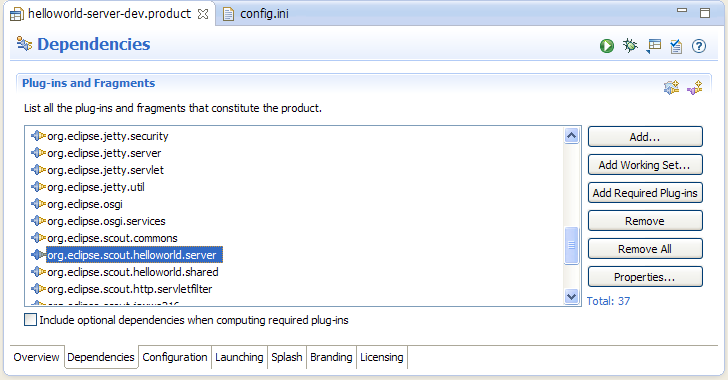
\includegraphics[width=14cm]{sdk_server_dev_product.png} 
\caption{The Eclipse product file editor showing file \java{helloworld-server-dev.product} of the ''Hello World'' application.
In the Dependencies tab shown above, the list of Eclipse plugins that are required for the server application are shown.
}
\index{Eclipse product file editor}
\figlabel{server_dev_product}
\end{figure}

For the case of the ''Hello World'' example we did not need to edit or change the product files generated by the Scout SDK. 
However, if your requirements are not met by the provided product files, you may use the Eclipse product file editor.
A screenshot of this editor is shown in \figref{server_dev_product} with the tab \element{Dependencies} opened.
In the tab Dependencies, the complete list of necessary plugins is provided.
Example plugins visible in \figref{server_dev_product} include the ''Hello World'' server and shared plugins, Scout framework plugins, and Jetty plugins.
The Jetty\footnote{
Jetty is web server with a small footprint: \url{http://www.eclipse.org/jetty/}.
} 
plugins are only needed to run the ''Hello World'' server application inside the Scout SDK.
Consequently, Jetty plugins are not listed as a dependency in the Scout server's production product file.

% ........................................................................... %
\subsection{Eclipse Configuration Files}
\index{Eclipse \filename{config.ini} file}
\seclabel{config_ini}

\begin{figure}
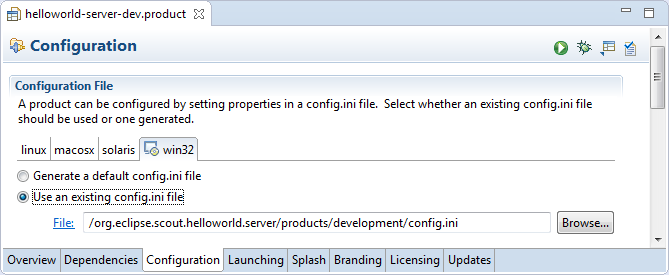
\includegraphics[width=14cm]{sdk_server_dev_product_config.png} \\ 

\includegraphics[height=5mm]{white_pixel.png} \\
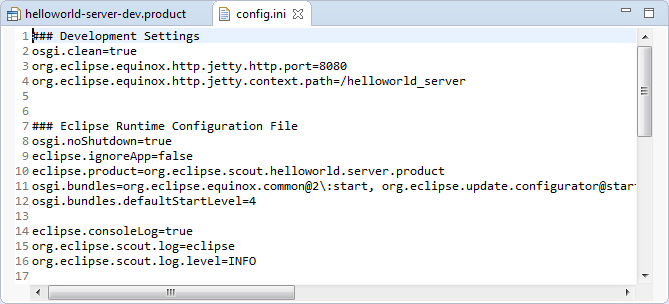
\includegraphics[width=14cm]{sdk_server_dev_configini.png} 
\caption{Above, the definition of the products \java{config.ini} in tab \element{Configuration} of the product file editor.
Below, the content of the configuration file of the ''Hello World'' server application is provided in a normal text editor.
}
\figlabel{server_dev_ini}
\end{figure}

Switching to tab \element{Configuration} in the product file editor, shows the selected radio button \element{Use an existing config.ini file} and the link to the configuration file provided in the \field{File} as shown in the upper part of \figref{server_dev_ini}.
Below, a part of the server's \filename{config.ini} file is shown.
Both the entry in the product file pointing to the configuration file, and the content of the \filename{config.ini} file has been generated by the Scout SDK during the initial project creation step.
As shown in the lower part of \figref{server_dev_ini}, Eclipse configuration files have the format of a standard property file.
The provided key value pairs are read at startup time if the \filename{config.ini} file can be found in folder \filename{configuration} by the Eclipse runtime.

% ........................................................................... %
\subsection{Scout Desktop Client Applications}

Having introduced Eclipse product files and configuration files based on the ''Hello World'' server application, we will now look at the different client applications in turn.
With Swing applications\footnote{
Swing is the primary Java UI technology: \url{http://en.wikipedia.org/wiki/Swing_\%28Java\%29}.
}
and SWT applications\footnote{
Standard Widget Toolkit (SWT): \url{http://en.wikipedia.org/wiki/Standard_Widget_Toolkit}.
}, two alternative UI technologies are currently available to build Scout desktop client applications.
More recently, JavaFX\footnote{
JavaFX is the most recent Java UI technology: \url{http://en.wikipedia.org/wiki/JavaFX}.
} 
is promoted as a successor to Swing and it is therefore likely, that Scout will provide JavaFX client applications in the future.

When we compare the product files for the Swing and the SWT client applications, it is apparent that both client applications share a large number of plugins.
Most importantly, the complete UI model and the business logic is identical for both client applications.
In other words, the value created by the Scout developer is contained in the two plugins \element{org.eclipse.scout.helloworld.client} and \element{org.eclipse.scout.helloworld.shared}.
To create an executable client application, we only need to combine these two plugins with a set of plugins specific to the desired UI technology.

After starting the ''Hello World'' Swing client or the corresponding SWT client application, the client application first reads the startup parameters from its \filename{config.ini} file.
Among other things, this client configuration file contains the parameter \java{server.url} to specify the URL to the ''Hello World'' server. 
After the startup of the ''Hello World'' client application, it can then connect to the ''Hello World'' server application using this address.

% ........................................................................... %
\subsection{Scout Web, Tablet and Mobile Clients}

For Scout web, tablet and  mobile clients, the Eclipse RAP framework\footnote{
Remote Application Platform (RAP): \url{http://www.eclipse.org/rap/}.
}
is used.
\index{RAP}
The RAP framework provides an API that is almost identical to the one provided by SWT and allows to use Java for server-side Ajax\footnote{
Asynchronous JavaScript and XML (AJAX): \url{http://en.wikipedia.org/wiki/Ajax_\%28programming\%29}.
}.
This setup implies that Scout tablet and mobile clients are not native clients but browser based\footnote{
To provide native clients with Scout, the simplest (commercial) option is most likely Tabris: \url{http://developer.eclipsesource.com/tabris/}
}.

Comparing the product file of the SWT client applications with the RAP application, we observe that the RAP development product does not include any SWT plugins, but a set of RAP and Jetty plugins.
In addition, the RAP product also contains the Scout mobile client plugins \element{org.eclipse.scout.rt.client.mobile} and \element{org.eclipse.scout.helloworld.client.mobile}.
These two plugins are responsible for transforming the UI model defined in the ''Hello World'' client plugin to the different form factors of tablet computers and mobile phones.

If you start the ''Hello World'' RAP application in your Scout SDK, you are launching a second server application in a Jetty instance on a different port than the ''Hello World'' server application.
As in the case of the desktop client applications, the RAP or Ajax server application knows how to connect to the ''Hello World'' server application after reading the parameter \java{server.url} from its \filename{config.ini} file.

% --------------------------------------------------------------------------- %
\section{The User Interface Part}
\seclabel{helloworld.userinterface.background}

Using the UI of the ''Hello World'' application we explain in this section how the Scout UI form model is represented in Java. 
We also describe how this representation is exploited by the Scout SDK to automatically manage the form data objects used for data transfer between Scout client and Scout server applications.
Finally, will have a brief look at internationalization\footnote{
Internationalization and localization, also called NLS support: \url{http://en.wikipedia.org/wiki/Internationalization_and_localization}.
} 
support of Scout for texts.

\lstinputlisting[
  label=\lstlabel{helloworld.mainbox},
  caption=The \java{DesktopForm} with its inner class \java{MainBox} containing the desktop box and message field,
  index={MainBox},
  linerange={19-22, 58-74, 90-91},
  float
]
{../code/helloworld/org.eclipse.scout.helloworld.client/src/org/eclipse/scout/helloworld/client/ui/forms/DesktopForm.java}

As discussed in \secref{helloworld.form} Scout forms consist of variables, the main box and a number of form handlers.
The main box represents the visible part of Scout's form model.
It may holds any number of form fields.
Using container fields such as group boxes, it is possible to define complex structures such as hierarchical UI models containing multiple levels.
In the Scout framework the forms structure is represented in the form of inner classes that are located inside of the \java{MainBox} class.
And the \wizard{New Form Field} of the Scout SDK fully supports this pattern.
\lstref{helloworld.mainbox} provides the concrete example using the the desktop form of the ''Hello World'' tutorial.

Using inner Java classes to model a form's content is a central aspect of the UI part of the Scout application model.
It allows the Scout SDK to easily parse the form's Java code on the fly and directly reflect changes to the form model in the Scout Explorer and the Scout Property View.
However, this is not the only benefit for the Scout SDK.
As form data objects hold all form variables and the values of all form fields contained in the form, the Scout SDK can keep the form data classes in sync with the forms of the application.
It is important to note that this mechanism only depends on the Java code of the form field class.
In consequence, the Scout SDK can update form field classes in the background even when form fields are manually coded into the form's Java class.
This includes adding all the necessary getter and setter methods to access the values of all the fields defined on a form.
As a result, Scout developers don't need to manually update form data objects when the UI model of a form is changed.
The Scout SDK takes care of this time consuming and error prone task.

\lstinputlisting[
  label=\lstlabel{helloworld.textproviderservice},
  caption=The \java{DefaultTextProviderService} class. Its getter method provides the path and the base name for the text property files,
  index={Text Provider Service},
  linerange={5-10},
  float
]
{../code/helloworld/org.eclipse.scout.helloworld.shared/src/org/eclipse/scout/helloworld/shared/services/common/text/DefaultTextProviderService.java}

\begin{figure}
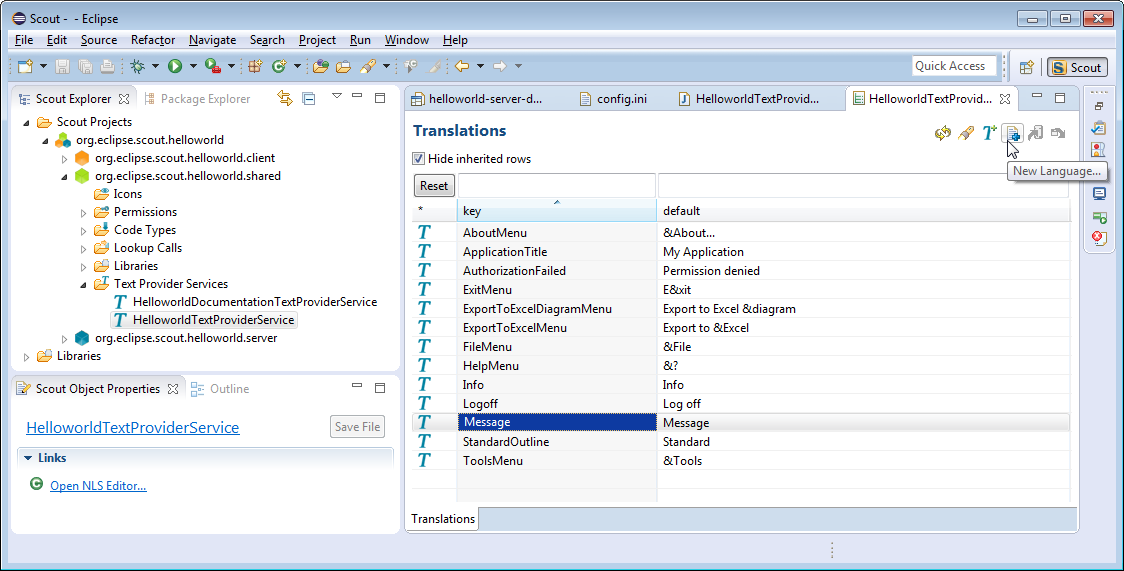
\includegraphics[width=14cm]{sdk_nls_editor.png} 
\caption{The NLS editor provided by the Scout SDK. This editor is opened via the \link{Open NLS Editor ...} in the Scout Object Properties of the \node{DefaultTextProviderService}.
}
\index{NLS editor}
\figlabel{nls_editor}
\end{figure}

When we did add the \field{Message} to the desktop form of the ''Hello World'' application we had to enter a new translation entry for the label of the message field as shown in \figref{helloworld_stringfield}.
The individual translation entries are then stored in language specific text property files.
To modify translated texts we can use the NLS editor provided by the Scout SDK.
To open this editor, select the green \node{shared} in the Scout Explorer and expand its \folder{Text Provider Services}.
Then, select the contained element \element{DefaultTextProviderService}.
As shown in \figref{nls_editor}, the NLS editor can then be opened using the \link{Open NLS Editor ...}.

To access the translated label field entry in the application, the Scout SDK generated the implementation of \java{getConfiguredLabel} using \java{TEXTS.get("Message")} as shown in \lstref{helloworld.mainbox}.
In the default Scout project setup, calling \java{TEXTS.get} uses the \java{DefaultTextProviderService} in the background.
This text provider service then defines the access path for the text property files to use for the translation.
To resolve the provided key, the user's locale settings are used to access the correct text property file.
As translated texts may need to be available in both client and server application, the NLS infrastructure including the text property files are located in the application's shared plugin.

\begin{figure}
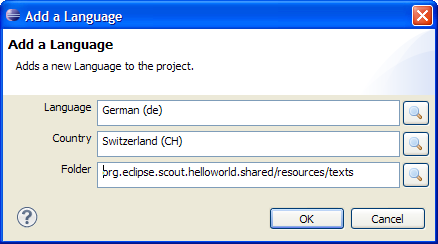
\includegraphics[height=4cm]{sdk_add_language_dialog.png} \hspace{0.5cm}
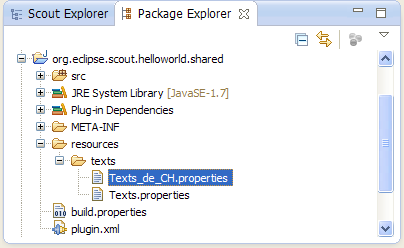
\includegraphics[height=4cm]{sdk_shared_plugin_language_file.png}
\caption{In the dialog \element{Add a Language} shown on the left side the desired language and localization can be specified.
On the right side, the location of property file \java{Texts\_de\_CH.properties} in the shared plugin of the ''Hello World'' application is shown.
}
\index{SDK Wizard!Add Translation Language}
\figlabel{adding_a_language}
\end{figure}

To add support for a new translated language, click on the corresponding icon of the NLS editor as shown in \figref{nls_editor}.
In the opened language dialog, add the desired language and country localization and the target directory as shown in \figref{adding_a_language}.
A new language properties file is then added to the shared plugin project as shown in \figref{adding_a_language}.
The new language is now available as an additional column in the NLS editor and as a separate tab in the dialog to add new translated texts shown in \figref{helloworld_stringfield}.

% --------------------------------------------------------------------------- %
\section{The Server Part}
\seclabel{helloworld.server.background}

In this background section we take a closer look at Scout services and calling service methods remotely.
We will first discuss the setup of an ordinary Scout service.
Then, the additional components to call service methods remotely are considered.
To explain the concepts in a concrete context, we use the setup of the \java{DesktopService} of our ''Hello World'' example.

% ........................................................................... %
\subsection{Scout Services}

Scout services are OSGi services\footnote{
A good introduction to OSGi services is provided by Lars Vogel's tutorial: \url{http://www.vogella.com/articles/OSGiServices/article.html}.
}
which in turn are defined by standard Java classes or interfaces.
Scout is just adding a convenience layer to cover typical requirements in the context of client server applications. 
To support Scout developers as much as possible, the Scout SDK offers wizards that generate the necessary classes and interfaces and also take care of service registration.

\lstinputlisting[
  label=\lstlabel{helloworld.desktop_service},
  caption=The server service class \java{DesktopService}.,
  linerange={8-15},
  float
]
{../code/helloworld/org.eclipse.scout.helloworld.server/src/org/eclipse/scout/helloworld/server/services/DesktopService.java}

All Scout services need to extend Scout's \java{AbstractService} class and implement their own corresponding interface.
This also applies to the ''Hello World'' desktop service according to \lstref{helloworld.desktop_service}.
As shown in \figref{helloworld_load_servicemethod}, this service can be located in the Scout Explorer under the blue server node in the \folder{Services}.

Before Scout services can be accessed and used, they need to be explicitly registered as a service in the correct place.
For this registration mechanism, Scout is using Eclipse extension points and extensions\footnote{
A good introduction to Eclipse extensions and extension points is provided in the Eclipse wiki: \url{http://wiki.eclipse.org/FAQ_What_are_extensions_and_extension_points\%3F}.
}
which are conceptually similar to electrical outlets and plugs.
And in order to work, as in the case of outlets and plugs, the plug must fit to the outlet.
In our ''Hello World'' example, the extension (plug) is represented by class \java{DesktopService} and the service extension point (outlet) is named \java{org.eclipse.scout.service.services}.
What makes the desktop service fit to the service extension point is the fact that its interface \java{IDesktopService} extends Scout's \java{IService} interface.

\begin{figure}
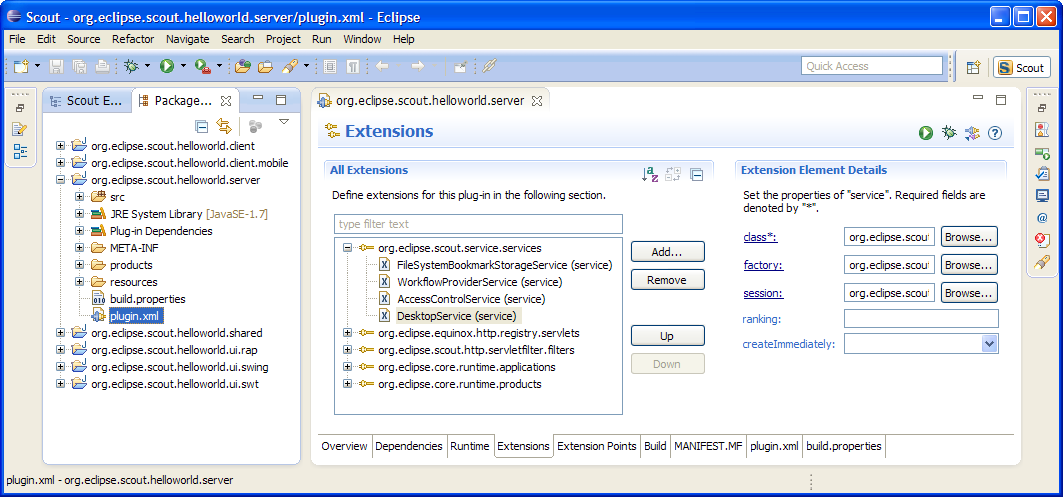
\includegraphics[width=14cm]{sdk_plugin_editor_desktopservice.png}
\caption{The Eclipse plugin editor for \java{plugin.xml} files.
In the tab \element{Extensions} the ''Hello World'' desktop service is registered under the extension point \java{org.eclipse.scout.service.services}.
}
\index{Eclipse plugin editor}
\figlabel{plugin_editor}
\end{figure}

\lstinputlisting[
  label=\lstlabel{helloworld.server_plugin_xml},
  caption=The registration of the \java{DesktopService} in the server's \java{plugin.xml} configuration file. The remaining content of the file has been omitted.,
  index={Plugin service registration},
  linerange={1-6,22-27,105-106},
  language=xml,
  float
]
{../code/helloworld/org.eclipse.scout.helloworld.server/plugin.xml}

The registration of the desktop service under the service extension point is then defined in the \filename{plugin.xml} file of the ''Hello World'' server plugin.
As shown in \figref{plugin_editor}, the \filename{plugin.xml} file is located in the root path of plugin \java{org.eclipse.scout.helloworld.server}.
To modify a \filename{plugin.xml}, you can either use the Eclipse plugin editor or your favorite text editor.
In \figref{plugin_editor}, the registration of the desktop service is shown in the \element{Extensions} tab of the plugin editor.
For the corresponding XML representation in the \filename{plugin.xml} file, see \lstref{helloworld.server_plugin_xml}.

% ........................................................................... %
\subsection{Scout Proxy Services}

In the ''Hello World'' application the \java{load} method of the desktop service is called remotely from the client.
But so far, we have only seen how the desktop service is implemented and registered in the server application.
To call server service methods remotely from Scout client applications, the Scout framework provides client proxy services and the service tunnel.
As the name implies, a client proxy service acts as a local proxy service (running in the Scout client application) of a server service (running remotely in the Scout server application).

\lstinputlisting[
  label=\lstlabel{helloworld.client_plugin_xml},
  caption=The registration of the \java{IDesktopService} proxy service in the client plugin of the ''Hello World'' application. This is the complete content of the client's \java{plugin.xml} file.,
  index={Plugin service registration},
  language=xml,
  float
]
{../code/helloworld/org.eclipse.scout.helloworld.client/plugin.xml}

Client proxy services are defined by a Java interface located in the shared plugin of the Scout application.
As shown in \lstref{helloworld.desktop_service} of the desktop service, this service interface is also implemented by the desktop service class in the server plugin.
Corresponding to the registration of the desktop service in the server plugin, client proxy services need to be registered in the client's \filename{plugin.xml} file.
The content of the ''Hello World'' client plugin configuration file is provided in \lstref{helloworld.client_plugin_xml}.
To create proxy services in Scout clients, the \java{ClientProxyServiceFactory} is used. 
This is also reflected in the extension defined in \lstref{helloworld.client_plugin_xml}.
Internally, this service factory then uses the service tunnel to create the local proxy services.

To call a remote service method from the Scout client application, we first need to obtain a reference to the proxy service.
Using the \java{SERVICES.getService} method with the interface \java{IDesktopService}, we can obtain such a reference as shown in \lstref{helloworld.viewhandler} for the view handler of the desktop form.
With this reference to the client's proxy service, calling methods remotely works as if the service would be running locally.
Connecting to the server, serializing the method call including parameters (and de serializing the return value) is handled transparently by Scout.

% --------------------------------------------------------------------------- %
\section{Add the Rayo Look and Feel}
\seclabel{helloworld.rayo.background}

Rayo has been designed in 2009 by BSI for its CRM\footnote{
Customer Relationship Management (CRM): \url{https://en.wikipedia.org/wiki/Customer_relationship_management}} 
application and contact center solution.
Since then, Rayo has been copied for Scout web applications and also adapted to work on touch/mobile devices.

The implementation of Rayo for desktop clients is based on the Java Synth look and feel\footnote{
Java Synth Look and Feel: \url{http://en.wikipedia.org/wiki/Synth_Look_and_Feel}
}.
However, in a few cases it was necessary to adjust some of the synth classes. 
In order to do this, the adapted classes are copied form the OpenJDK implementation\footnote{
OpenJDK is an open source implementation of the Java platform: \url{http://openjdk.java.net/}.
}
As OpenJDK is licenced under the GNU General Public Licence (GPL) with a linking exception it is not possible to distribute Rayo under the Eclipse Public Licence.
That is why Rayo is not initially contained in the Eclipse Scout package but needs to be downloaded from the Eclipse Marketplace.
Fortunately, there is still no restriction to use Rayo in commercial products.
The only remaining restriction applies to modifying Rayo for commercial products.
In this case you will be obliged to redistribute your modified version of Rayo under the same licence (GPL with classpath exception).

With Eclipse Scout 3.8 (Juno), the Scout framework also allows to build web clients based on Eclipse RAP.
Great care has been taken to ensure, that the look and feel for Scout web applications matches the look and feel of the desktop as closely as possible.
As RAP is already distributed under the EPL licence the Rayo for web apps is directly contained in the Scout package.
TODO: Describe what to change to use RAP default look and feel

A similar approach was chosen for Rayo on tablets and mobile devices that are supported with Eclipse Scout 3.9 (Kepler).
For such devices optimized components are used to take into account the smaller screens and the absence of a mouse (no context menus!)
But as far as possible, the Rayo look and feel also applies to touch devices.
TODO: Pointer to more info regarding mobile devices.

% --------------------------------------------------------------------------- %
\section{Exporting the Application}
\seclabel{helloworld_export_background}

In this background section we look at the content and organisation of the two WAR files generated by the Scout SDK \wizard{Export Scout Project}.
The first WAR file holds the Scout server including a landing page to download the Scout desktop client.
The desktop client is provided in the form of a standalone ZIP file.
In the second WAR file, the Ajax server based on Eclipse RAP is contained.
This Ajax server provides the URLs that can be accessed by web browsers running on desktop computers or tablet and mobile devices.

\begin{figure}
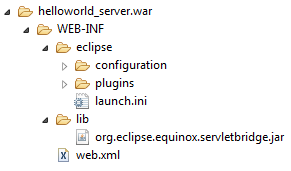
\includegraphics[height=5cm]{helloworld_server_war.png} \hspace{5mm}
\includegraphics[height=5cm]{helloworld_server_war_eclipse.png}
\caption{The organisation of the ''Hello World'' server WAR file.
The right side reveals the location of the \java{config.ini} file and the application's plugin files} 
\figlabel{helloworld_server_war}
\end{figure}

The content and its organisation of the exported WAR files was not specifically designed for Scout applications. 
Rather, it is defined according to server-side Equinox\footnote{
See \appref{osgi_basics} for more information regarding server-side Equinox.
},
the typical setup for running Eclipse based server applications on a web server.
Using file \filename{helloworld_server.war} as a concrete example, we will first describe the general organisation of the WAR file.
Then, we introduce individual artefacts of interest that are contained in this WAR file.

The explicit organisation of the server WAR file is shown in \figref{helloworld_server_war}.
From the left hand side of the figure we can see that on the top level only folder \filename{WEB-INF} exists in the WAR file.
This folder contains all files and directories that are private to the web application.
Inside, the web deployment descriptor file \filename{web.xml} as well as the directories \filename{lib} and \filename{eclipse} are located.
While the \filename{web.xml} file and directory \filename{lib} are standard for servlet based based applications\footnote{
See \appref{javaee_basics} for more information regarding servlets.
},
directory \filename{eclipse} contains all necessary artefacts for servlet based Eclipse applications\footnote{
See \appref{osgi_basics} for more information regarding server-side Eclipse applications (server-side Equinox). 
}.
Such as Eclipse Scout server applications.

On the right hand side of \figref{helloworld_server_war} the eclipse specific content of the WAR file is shown.
From top to bottom we find the configuration file \filename{config.ini} introduced in \secref{config_ini}.
In folder \filename{plugins} the necessary plugins that constitute the eclipse application are located where the plugins are available in the form of JAR files\footnote{
JAR files contain a set of Java classes and associated resources. \url{http://en.wikipedia.org/wiki/JAR_\%28file_format\%29}.
}.
This includes plugins for servlet management, the eclipse platform including the servlet bridge, the scout framework parts and of course our ''Hello World'' server and shared plugin.
These ''Hello World'' jar files exactly match with the plugin projects discussed in \secref{create_project_simple_background}.

\begin{figure}
\includegraphics[height=9cm]{helloworld_server_war_plugin.png} 
\caption{The content of the ''Hello World'' server plugin contained in the \java{helloworld\_server.war} file.
The necessary files for the download page including the zipped client application are in the \java{resources/html} directory.} 
\figlabel{helloworld_server_plugin}
\end{figure}

\lstinputlisting[
  label=\lstlabel{helloworld.server_plugin_xml.resourceservlet},
  caption=The configuration of the server's resource servlet in the \java{plugin.xml} configuration file. The remaining content of the file has been omitted.,
  linerange={1-3,28-30,51-62,104-106},
  language=xml,
  float
]
{../code/helloworld/org.eclipse.scout.helloworld.server/plugin.xml}

In \figref{helloworld_server_plugin} some of the content of the ''Hello World'' server plugin is shown.
The first thing to note is that the plugin file conforms to the JAR file format including a \filename{META-INF/MANIFEST.MF} file and the directory tree containing the Java class files, as the \filename{DesktopService.class} implemented in \secref{helloworld.server} of the ''Hello World'' tutorial.
In folder \filename{resources/html} the necessary files for the download page shown in \figref{helloworld_running_download} including the zipped desktop client are contained.
To access this download page the Scout server's resource servlet \java{ResourceServlet} is responsible.
It is registered under the servlet registry as shown in \lstref{helloworld.server_plugin_xml.resourceservlet}.
With setting "/" of the \java{alias} parameter the download page becomes available under the root path of the Scout server application.
For the mapping to the contents \filename{resources/html} the parameter \java{bundle-path} is used.

\begin{figure}
\includegraphics[height=8cm]{helloworld_server_plugin.png} 
\caption{The ''Hello World'' server plugin shown in the Eclipse package explorer.
The files for the download page are located under \java{resources/html}.} 
\figlabel{helloworld_server_explorer}
\end{figure}

Revisiting the ''Hello World'' server plugin project in the Eclipse package explorer as shown in \figref{helloworld_server_explorer}, we can see how the plugin project elements are transformed and copied into the JAR file.
Examples files are \filename{plugin.xml} and \filename{MANIFEST.MF} as well as static HTML content of the download page (files \filename{index.html} and \filename{scout.gif}).
The zipped client is missing of course.
It is assembled, zipped and added into the Scout server JAR file by the \wizard{Export Scout Project} of the Scout SDK.
In case you need to change/brand/amend the download page for the desktop client, you have now learned where to add and change the corresponding HTML files.

% --------------------------------------------------------------------------- %
\section{Deploying to Tomcat}
\seclabel{helloworld.tomcat.background}

In this section we will discuss two common pitfalls when working with the Scout IDE and Tomcat.
The symptoms linked to these problems are Scour server applications that are not starting or Scout applications that fail to properly update.

In usual culprit behind Scout server applications that fail to start is a blocked port 8080.
This setting can be created when we try to run both the Jetty web server inside the Scout SDK and the local Tomcat instance.
In consequence, either Jetty or Tomcat is not able to bind to port 8080 at startup which makes it impossible for a client to connect to the right server.
To avoid such conflicts, make sure that you always stop the Scout server application in the Scout SDK (effectively killing Jetty) before you restart your Tomcat server.
Alternatively, you can assign two different ports to your Jetty webserver and your Tomcat webserver.

To modify Jetty's port number in the Scout SDK you have to update the corresponding properties in the \filename{config.ini} files of the development products of your Scout server application and all client applications.
In the Scout server's \filename{config.ini} file the property is named \java{org.eclipse.equinox.http.jetty.http.port}, in the client \filename{config.ini} files the relevant property is called \java{server.url}.
To change the port number to 8081 for the ''Hello World'' example in the Scout SDK you could use the following lines in the individual \filename{config.ini} files.

\begin{tabular}{ll}
 Scout Server         & org.eclipse.equinox.http.jetty.http.port=8081              \\
 Scout Desktop Client & server.url=http://localhost:8081/helloworld\_server/process \\
 Scout Ajax Server    & server.url=http://localhost:8081/helloworld\_server/ajax
\end{tabular}

The second pitfall is connected to a web application that seems to refuse to update to the content of a freshly generated WAR file.
At times it seems that your changes to a deployed WAR file do not find their way to the application actually running. 
In many cases this is caused by a cached instance of the previous version of your application located in Tomcat's working directory.
To save yourself much frustration, it often helps just to clear Tomcat's working directory and restart Tomcat.
For this, you may follow the following procedure.

\begin{enumerate}
  \item Stop the Tomcat web server
  \item Go to folder \filename{work/Catalina/localhost}
  \item Verify that you are not in Tomcat's \filename{webapps} folder
  \item Delete all files and directories in folder \filename{work/Catalina/localhost}
  \item Start the Tomcat web server
\end{enumerate}

How you start and stop Tomcat depends on the platform you are running it. 
If you have installed Tomcat on a Windows box according to \appref{install_tomcat} it will be running as a service.
This means that to stop the Tomcat web server you need to stop the corresponding Windows service.
For starting and stopping Tomcat on Mac/Linux/Unix systems, you can use the command line script files \filename{startup.sh} and \filename{shutdown.sh} located in Tomcat's subdirectory \filename{bin}.

For those interested in more advanced aspects of Apache Tomcat we recommend the article ''More about the Cat'' by Chua Hock-Chuan\footnote{
More about the Cat: \url{http://www.ntu.edu.sg/home/ehchua/programming/howto/Tomcat_More.html}.
}.

% --------------------------------------------------------------------------- %

\ifx\wholebook\relax\else
   \begin{thebibliography}{99}
  \addcontentsline{toc}{chapter}{Bibliography}
  
  % add/insert books in alphabetical order of 1st author
  
  \bibitem{batessierra05}
    \textit{Bert Bates, Kathy Sierra},
	\textbf{Head First Java} 2nd edition, 
	O'Reilly Media, 2005.

  \bibitem{bloch08} 
    \textit{Joshua Bloch},
    \textbf{Effective Java} 2nd edition, 
	Addison-Wesley, 2008.
	
  \bibitem{eckel06}
    \textit{Bruce Eckel},
	\textbf{Thinking in Java} 4th edition, 
	Prentice Hall International, 2006.

\end{thebibliography}

   \end{document}
\fi

% =========================================================================== %

% =========================================================================== %
% Scout Runtime
% =========================================================================== %

\ifx\wholebook\relax\else
  \documentclass[a4paper,10pt,twoside]{book}
  %=============================================================================%
% Common things, settings, packages to include
%=============================================================================%

\usepackage{graphicx}
\usepackage{color}
\usepackage{makeidx}
\usepackage{ifpdf}
\usepackage{verbatim}

% --------------------------------------------------------------------------- %
% Setting up stuff depeding on output format
% --------------------------------------------------------------------------- %

\ifpdf
  % special settings for pdf mode
  \usepackage[colorlinks]{hyperref}
  \usepackage{courier}
  
  \hypersetup{
    colorlinks,
    linkcolor=darkblue,
    citecolor=darkblue,
    pdftitle={The Eclipse Scout Book},
    pdfauthor={The Scout Community},
    pdfkeywords={Enterprise Framework, Eclipse, Java, Client-Side, Rich Client, Web Client, Mobile},
    pdfsubject={Computer Science}
  }
  
  \usepackage{caption}
  \captionsetup{margin=10pt,font=small,labelfont=bf}
\else
  % special stuff for html mode
  \usepackage[tex4ht]{hyperref}
\fi

% --------------------------------------------------------------------------- %
% Setting up printing range
% --------------------------------------------------------------------------- %

\parindent 1cm
\parskip 0.2cm
\topmargin 0.2cm
\oddsidemargin 1cm
\evensidemargin 0.5cm
\textwidth 15cm
\textheight 21cm

% --------------------------------------------------------------------------- %
% Setting up listings
% --------------------------------------------------------------------------- %

\usepackage{listings}
 
\definecolor{darkviolet}{rgb}{0.5,0,0.4}
\definecolor{darkgreen}{rgb}{0,0.4,0.2} 
\definecolor{darkblue}{rgb}{0.1,0.1,0.9}
\definecolor{darkgrey}{rgb}{0.5,0.5,0.5}
\definecolor{lightblue}{rgb}{0.4,0.4,1}
\definecolor{lightgray}{rgb}{0.97,0.97,0.97}

\renewcommand{\lstlistlistingname}{List of Listings}

% general settings
\lstset{
  basicstyle=\small\ttfamily,
  columns=fullflexible,
  breaklines=true,
  breakindent=10pt,
  prebreak=\mbox{{\color{blue}\tiny$\searrow$}},
  postbreak=\mbox{{\color{blue}\tiny$\rightarrow$}},
  showstringspaces=false,
  backgroundcolor=\color{lightgray}
}

% settings for xml files
\lstdefinelanguage{xml}
{
  commentstyle=\color{darkgrey}\upshape,
  morestring=[b]",
  morestring=[s]{>}{<},
  morecomment=[s]{<?}{?>},
  stringstyle=\color{black},
  identifierstyle=\color{darkblue},
  keywordstyle=\color{cyan},
  morekeywords={xmlns,name,point,factory,class}% list your attributes here
}

% settings for ini files
\lstdefinelanguage{ini}
{
  morecomment=[f][\color{darkgrey}\upshape][0]\#, % # is comment iff it's the first char on the line
  stringstyle=\color{black}
}

% default settings (for java files)
\lstset{
  language=Java,
  emphstyle=\color{red}\bfseries,
  keywordstyle=\color{darkviolet}\bfseries,
  commentstyle=\color{darkgreen},
  morecomment=[s][\color{lightblue}]{/**}{*/},
  stringstyle=\color{darkblue},
}

% --------------------------------------------------------------------------- %
% cross reference macros
% --------------------------------------------------------------------------- %
\newcommand{\applabel}[1]{\label{apx:#1}}
\newcommand{\chalabel}[1]{\label{cha:#1}}
\newcommand{\seclabel}[1]{\label{sec:#1}}
\newcommand{\lstlabel}[1]{\label{lst:#1}}
\newcommand{\figlabel}[1]{\label{fig:#1}}
\newcommand{\tablabel}[1]{\label{tab:#1}}

\newcommand{\appref}[1]{Appendix~\ref{apx:#1}}
\newcommand{\charef}[1]{Chapter~\ref{cha:#1}\xspace}
\newcommand{\secref}[1]{Section~\ref{sec:#1}}
\newcommand{\lstref}[1]{Listing~\ref{lst:#1}\xspace}
\newcommand{\figref}[1]{Figure~\ref{fig:#1}\xspace}
\newcommand{\tabref}[1]{Table~\ref{tab:#1}\xspace}

% --------------------------------------------------------------------------- %
% graphics paths
% --------------------------------------------------------------------------- %
\graphicspath{
  {figures/}
  {Introduction/figures/}
}

%=============================================================================%

  \pagestyle{headings}
  \graphicspath{{figures/} {../figures/}}
  \begin{document}
  \sloppy
\fi


% --------------------------------------------------------------------------- %
\chapter{Scout Runtime}
\chalabel{runtime}

One of the primary goals of the Scout runtime framework is to let the application developer focus on implementing business requirements. 
To support this goal, the Scout runtime defines an application model that covers a wide variety of recurring aspects of business applications.

Developing complex user interface, dealing with input validation, client server communication, handling of codes, permissions, user authentication, logging, and accessing data bases or backend systems using web services are all aspects that are covered by Scout.
On the other hand, business modeling, a persistence layer, role models for user authorisation are outside of the scope of the Scout runtime.
This is by design, as Scout does not cover domains already addressed by powerful and well established open source frameworks.

Where possible, Scout relies on the standards defined by the OSGi/Eclipse platform and a small subset of J2EE components. 
Typically, just a thin convenience layer is added by Scout. 
This helps the beginner to pick up Scout concepts more quickly and -- at the same time -- offers the necessary flexibility to developers that are already familiar with those technologies. 

In this chapter we first discuss the framework scope based on the integration of a Scout application in a typical enterprise setup.
Then, we describe the internal architecture of Scout applications and highlight the difference of the architecture for scenarios involving desktop clients and web/mobile clients.
As the multi-frontend support for Scout applications is one of the most important featues of the Scout application model a specific section is dedicated to this feature.
Finally, the basic building blocks of a Scout application -- the Scout server, the Scout client, and the client server communication -- are described individually.


% --------------------------------------------------------------------------- %
\section{Enterprise Integration}
\seclabel{enterprise_integration}

\begin{figure}
\includediagram{14cm}{scout_integration}
\caption{The recommended usage of the Scout framework for enterprise applications.}
\figlabel{scout_integration_enterprise}
\end{figure}

The scope of the Scout framework is best explained in the context of an enterprise setup as shown in \figref{scout_integration_enterprise}. 
From

not persistence, not business entity modeling, not ?
but user interaction handling, business rules, accessing existing services offered through enterprise service bus, transparent client server communication

% --------------------------------------------------------------------------- %
\section{Application Architecture}
\seclabel{application_architecture}
needs text

\noindent Existing Documentation
\begin{itemize}
  \item wiki \url{http://wiki.eclipse.org/Scout/Concepts}
\end{itemize}

\begin{figure}
\includediagram{14cm}{scout_app_architecture_desktop}
\caption{The architecture of a typical Scout client server application.
On the left side, a Scout desktop client is depicted.}
\figlabel{scout_app_architecture_desktop}
\end{figure}

Architecture including desktop clients.

\begin{figure}
\includediagram{14cm}{scout_app_architecture_web}
\caption{A typical Scout client server setup including web and mobile clients.}
\figlabel{scout_app_architecture_web}
\end{figure}

Architecture when wordking with Ajax server for web applications

% --------------------------------------------------------------------------- %
\section{Multi-Frontend Support}

two important aspects: 1) same app running on many devices 2) effective risk reduction strategy: no mixing of business logic an ui tech code, deciding for the 'wrong' framwork not so bad any more

% --------------------------------------------------------------------------- %
\section{The Scout Client}
needs text

 large collection of mature UI components.
 Scout supports various UI technologies out of the box. 
 Depending on your needs, you decide to build applications for
mobile devices, the browser or the desktop. Mobile and
web applications are based on Eclipse RAP. Desktop clients
are based on either Swing or SWT.

internationalization, link to packaging with client, shared, ui tech, framwork + other bundles. 


\noindent Existing Documentation
\begin{itemize}
  \item scout concept wiki: client plug-in \url{http://wiki.eclipse.org/Scout/Concepts/Separation_UI_and_GUI}
\end{itemize}

% --------------------------------------------------------------------------- %
\section{The Scout Server}

For seamless integration into a service-oriented IT architecture, Scout offers direct support for Web services based on
JAX-WS. To access relational databases other than Apache
Derby, connectors are also available for non-EPL compatible databases such as Oracle, MySql, PostgreSQL or DB2

link to packaging with server, shared, framwork + other bundles

\noindent Existing Documentation
\begin{itemize}
  \item scout concept wiki: server plug-in \url{http://wiki.eclipse.org/Scout/Concepts/Server_Plug-In}
  \item scout concept wiki: security \url{http://wiki.eclipse.org/Scout/Concepts/Security}
\end{itemize}

% --------------------------------------------------------------------------- %
\section{Communication and Shared Components}
needs text

service tunnel

Icons Class that contains as static members the icons that are available. 
Permissions are.
Enumerations are codes A CodeType is a structure to represent a tree key-code association. 
They are used in SmartField and SmartColumn. 
Texts is a convenience class to access the Text Provider Services used for the localization of the texts in the user interface. 


\noindent Existing Documentation
\begin{itemize}
  \item forum tech background questions \url{http://www.eclipse.org/forums/index.php/t/299623/}
  \item concept wiki communication \url{http://wiki.eclipse.org/Scout/Concepts/Communication}
  \item concept wiki shared \url{http://wiki.eclipse.org/Scout/Concepts/Shared_Plug-In}
\end{itemize}

same pointer in onedaytutorial and server


\ifx\wholebook\relax\else
   \begin{thebibliography}{99}
  \addcontentsline{toc}{chapter}{Bibliography}
  
  % add/insert books in alphabetical order of 1st author
  
  \bibitem{batessierra05}
    \textit{Bert Bates, Kathy Sierra},
	\textbf{Head First Java} 2nd edition, 
	O'Reilly Media, 2005.

  \bibitem{bloch08} 
    \textit{Joshua Bloch},
    \textbf{Effective Java} 2nd edition, 
	Addison-Wesley, 2008.
	
  \bibitem{eckel06}
    \textit{Bruce Eckel},
	\textbf{Thinking in Java} 4th edition, 
	Prentice Hall International, 2006.

\end{thebibliography}

   \end{document}
\fi

% =========================================================================== %

% =========================================================================== %
% Scout Tooling
% =========================================================================== %

\ifx\wholebook\relax\else
  \documentclass[a4paper,10pt,twoside]{book}
  %=============================================================================%
% Common things, settings, packages to include
%=============================================================================%

\usepackage{graphicx}
\usepackage{color}
\usepackage{makeidx}
\usepackage{ifpdf}
\usepackage{verbatim}

% --------------------------------------------------------------------------- %
% Setting up stuff depeding on output format
% --------------------------------------------------------------------------- %

\ifpdf
  % special settings for pdf mode
  \usepackage[colorlinks]{hyperref}
  \usepackage{courier}
  
  \hypersetup{
    colorlinks,
    linkcolor=darkblue,
    citecolor=darkblue,
    pdftitle={The Eclipse Scout Book},
    pdfauthor={The Scout Community},
    pdfkeywords={Enterprise Framework, Eclipse, Java, Client-Side, Rich Client, Web Client, Mobile},
    pdfsubject={Computer Science}
  }
  
  \usepackage{caption}
  \captionsetup{margin=10pt,font=small,labelfont=bf}
\else
  % special stuff for html mode
  \usepackage[tex4ht]{hyperref}
\fi

% --------------------------------------------------------------------------- %
% Setting up printing range
% --------------------------------------------------------------------------- %

\parindent 1cm
\parskip 0.2cm
\topmargin 0.2cm
\oddsidemargin 1cm
\evensidemargin 0.5cm
\textwidth 15cm
\textheight 21cm

% --------------------------------------------------------------------------- %
% Setting up listings
% --------------------------------------------------------------------------- %

\usepackage{listings}
 
\definecolor{darkviolet}{rgb}{0.5,0,0.4}
\definecolor{darkgreen}{rgb}{0,0.4,0.2} 
\definecolor{darkblue}{rgb}{0.1,0.1,0.9}
\definecolor{darkgrey}{rgb}{0.5,0.5,0.5}
\definecolor{lightblue}{rgb}{0.4,0.4,1}
\definecolor{lightgray}{rgb}{0.97,0.97,0.97}

\renewcommand{\lstlistlistingname}{List of Listings}

% general settings
\lstset{
  basicstyle=\small\ttfamily,
  columns=fullflexible,
  breaklines=true,
  breakindent=10pt,
  prebreak=\mbox{{\color{blue}\tiny$\searrow$}},
  postbreak=\mbox{{\color{blue}\tiny$\rightarrow$}},
  showstringspaces=false,
  backgroundcolor=\color{lightgray}
}

% settings for xml files
\lstdefinelanguage{xml}
{
  commentstyle=\color{darkgrey}\upshape,
  morestring=[b]",
  morestring=[s]{>}{<},
  morecomment=[s]{<?}{?>},
  stringstyle=\color{black},
  identifierstyle=\color{darkblue},
  keywordstyle=\color{cyan},
  morekeywords={xmlns,name,point,factory,class}% list your attributes here
}

% settings for ini files
\lstdefinelanguage{ini}
{
  morecomment=[f][\color{darkgrey}\upshape][0]\#, % # is comment iff it's the first char on the line
  stringstyle=\color{black}
}

% default settings (for java files)
\lstset{
  language=Java,
  emphstyle=\color{red}\bfseries,
  keywordstyle=\color{darkviolet}\bfseries,
  commentstyle=\color{darkgreen},
  morecomment=[s][\color{lightblue}]{/**}{*/},
  stringstyle=\color{darkblue},
}

% --------------------------------------------------------------------------- %
% cross reference macros
% --------------------------------------------------------------------------- %
\newcommand{\applabel}[1]{\label{apx:#1}}
\newcommand{\chalabel}[1]{\label{cha:#1}}
\newcommand{\seclabel}[1]{\label{sec:#1}}
\newcommand{\lstlabel}[1]{\label{lst:#1}}
\newcommand{\figlabel}[1]{\label{fig:#1}}
\newcommand{\tablabel}[1]{\label{tab:#1}}

\newcommand{\appref}[1]{Appendix~\ref{apx:#1}}
\newcommand{\charef}[1]{Chapter~\ref{cha:#1}\xspace}
\newcommand{\secref}[1]{Section~\ref{sec:#1}}
\newcommand{\lstref}[1]{Listing~\ref{lst:#1}\xspace}
\newcommand{\figref}[1]{Figure~\ref{fig:#1}\xspace}
\newcommand{\tabref}[1]{Table~\ref{tab:#1}\xspace}

% --------------------------------------------------------------------------- %
% graphics paths
% --------------------------------------------------------------------------- %
\graphicspath{
  {figures/}
  {Introduction/figures/}
}

%=============================================================================%

  \pagestyle{headings}
  \graphicspath{{figures/} {../figures/}}
  \begin{document}
  \sloppy
\fi

% --------------------------------------------------------------------------- %
\chapter{Scout Tooling}
\chalabel{tooling}

In addition to the Scout runtime framework presented in the previous chapter, Eclipse Scout also includes a comprehensive tooling, the Scout SDK. 
Thanks to this tooling, developing Scout applications is made simpler, more productive and also more robust. 
Initially, a solid understanding of the Java language is sufficient to start developing Scout applications and only a rough understanding of the underlying Eclipse/OSGi/JEE technologies is required. 

The Scout SDK consists of navigation support for the application model defined by the Scout runtime and provides many intuitive component wizards. 
This creates an ideal environment to beginners for building complete, high-quality Scout applications. 
Typically, Java developers only need a few days of Scout training to start creating their own advanced client server business applications. 

The Scout SDK also helps developers to become more productive.
Many repetitive and error prone tasks run automatically in the background or are taken care of by the component wizards of the Scout SDK. 
This starts with the initial creation of a Scout client server application, continues with the wizards to create complete dialogs and pages and includes the automatic management of the data transfer objects needed by the client server communication.

Finally, the application code created by the Scout SDK wizards helps to ensure that the resulting Scout application has a consistent and robust code base and is well aligned with the application model defined by the Scout runtime framework.

% --------------------------------------------------------------------------- %
\section{The Scout SDK}
\index{Scout SDK}

The Scout SDK is added to the Eclipse IDE in the form of the Scout perspective\footnote{
See \appref{eclipse_perspective} for additional information regarding Eclipse IDE perspectives. 
}.
With the Scout Explorer and Scout Objects Properties, two view parts are contained in the Scout perspective. 
Additionally, the Scout SDK contains a comprehensive set of wizards that support the developer in creating Scout application components. 

The Scout Explorer view allows the developer to navigate the complete Scout application model. 
Once an element in the Scout Explorer is selected, the Scout Object properties view allows to view and change selected properties of the selected element. 
Depending on the selected element in the Scout Explorer, the Scout SDK offers appropriate context menus to start the related wizards.

\begin{figure}
\includegraphics[width=14cm]{scout_sdk_perspective.png} 
\caption{The Scout SDK perspective. On the left hand side the Eclipse Scout Explorer and the Scout Object Properties view are visible.}
\figlabel{scout_sdk_perspective}
\end{figure}

\figref{scout_sdk_perspective} provides a screenshot of the Scout SDK perspective. 
In the Eclipse Scout Explorer shown in the upper left part of the screenshot, the message field in the desktop form of the ''Hello World'' application is selected. 
In the Scout Object Properties located below, the message field's appearance, layout and behaviour properties are displayed. 
On the right side, the corresponding source code is loaded in a Java editor. 

When the developer changes a property of the selected element, the Java code is updated accordingly. 
For example, clicking the \property{Mandatory} in the Scout Object Properties of the message field will insert the method \java{getConfiguredLabel} to the message field's class. 
This demonstrates how the Scout SDK directly works on the Java source code. 
In fact, the Java source code is the only artefact relevant for the Scout SDK to 'understand' the Scout application model. 
Taking advantage of this setup, the Scout SDK implements a full round-trip-engineering from creating the Java code for Scout application components, parsing code changes in the background, and displaying the current implementation of the Scout application in the Scout Explorer and the Scout Object Properties.

Thanks to the round-trip-engineering provided by the Scout SDK, the information presented in the Scout Explorer and the Scout Object Properties always stay in sync with the Java code of the Scout application.
To illustrate this, we will re-use the ''Hello World'' Scout project from \charef{helloworld}. 
Start the Eclipse IDE with the workspace containing the ''Hello World'' application.
Then, navigate to method \java{getConfiguredLabel} as shown in \figref{scout_sdk_perspective}, and add the java snippet shown below to the class \java{MessageField}. 

\begin{lstlisting}[backgroundcolor=\color{white}]
    @Override
    protected boolean getConfiguredMandatory() {
        return true;
    }
\end{lstlisting}

After having saved the code change, you can observe that the \property{Mandatory} in the section Behaviour of the message field's Scout Object properties has changed its state. 
The font of its label is now presented in bold face and underlined, the checkbox is ticked and a red minus icon is shown on the right side of the property. 
Obviously, the Scout SDK is directly operating on the project's source code and does not rely or need any external meta data. 
This provides the flexibility to develop Scout applications with or without the support of the Scout SDK. 
And this choice offered to the Scout developer is one of the most important features provided by the Scout SDK. 
The Scout developer may take advantage of the development support provided by the Scout SDK without being restricted by the Scout tooling in any way.

Technically, the Scout SDK is a set of Eclipse plugins that operate on top of the Eclipse JDT and the Eclipse PDE projects.
The Java Development Tools (JDT)\footnote{
See the Eclipse JDT project page for details: \url{http://www.eclipse.org/jdt/}.
} 
contain a Java IDE supporting the development of any Java application, 
and the Plugin Development Environment (PDE)\footnote{
See the Eclipse PDE project page for details: \url{http://www.eclipse.org/pde/}.
}
provides tools to create, develop, test, debug, build and deploy Eclipse plugins, and additional artefacts relevant for Eclipse based applications. 
As in the case of the Scout Runtime, the plugins representing the Scout SDK, the JDT and the PDE are all located in the \filename{plugins} directory your Eclipse installation and named \filename{org.eclipse.scout.sdk.*}, \filename{org.eclipse.jdt.*} and \filename{org.eclipse.pde.*} . 

% --------------------------------------------------------------------------- %
\section{The Scout Explorer}
\index{Scout Explorer}

The Scout Explorer view is responsible for the navigation support within the Scout application model. 
This navigation support is presented in the form of a tree view and includes the client with its UI components, the server and the shared part of a Scout application. 
It also includes all Scout application modules of modular Scout applications\footnote{
See \secref{multi_module_apps} for more information regarding multi module Scout applications.
}.
For the actual navigation in the tree representing the Scout application both the mouse or the keyboard can be used. 

To expand or collapse a selected node in the Scout Explorer, you may click on the tiny \icon{plus} or the \icon{minus} presented to the left of the node.
Alternatively, you can also use the \key{Right} or the \key{Left}.

Once a node in the tree is selected, the Scout Object Properties view presents the associated configuration of the selected element. 
If the selected element represents a specific application model component, the corresponding Java source code can be accessed through a double click on the node, or hitting the \key{Enter}. 

The navigation tree provided in the Scout Explorer view also allows the developer to add elements to your application.
Depending on the selected node in the tree, the Scout SDK allows to start the applicable Scout SDK wizards using corresponding context menus. 
The wizards support the creation of application components, such as dialogues on the client side or services on the server side by generating the necessary Java code.

\begin{figure}
\includegraphics[width=6.5cm]{explorer_client.png} 
\caption{The Scout Explorer view. The white nodes below the expanded client node represent the supported UI technologies.}
\figlabel{explorer_client}
\end{figure}

In \figref{explorer_client} the top level organisation of the client application model is shown as it is represented in the Scout Explorer.
All client specific elements are located under the selected orange client node \element{org.eclipsescout.helloworld.client}. 
Right below, the three white UI plugins are located that represent the support for the corresponding UI technologies for Swing, SWT and Eclipse RAP. 
The orange \node{org.eclipsescout.helloworld.client.mobile} contains all elements that are specific to mobile devices such as the \java{MobileHomeForm}

Specific nodes for the client session and the desktop of the Scout client allow access to the corresponding Scout application model components. 
While the client session is the main entry point for client-server communication, the desktop represents the root component of the visible part of a Scout client applications. 
Below, a set of folders group additional client model components according to their type. 
The forms folder for example holds all available forms, such as the desktop form that we have seen in the ''Hello World!'' tutorial\footnote{
See \secref{initial_helloworld} for a description of many of these elements.
}. 

\begin{figure}
\includegraphics[width=7cm]{explorer_shared.png} 
\caption{The Scout Explorer view with the expanded shared node.}
\figlabel{explorer_shared}
\end{figure}

A screenshot of the expanded green shared node \element{org.eclipsescout.helloworld.} is provided in \figref{explorer_shared}. 
As the name ''shared'' suggests, the corresponding plugin holds all application components that are required for both the Scout client and the Scout server application. 
This includes texts, icons, enumeration or codes, permissions, lookup calls. 
As shown in \figref{explorer_shared}, a separate folder for each resource type is provided under the shared node.
 
\begin{figure}
\includegraphics[height=6.8cm]{explorer_server.png} \hspace{5mm} 
\includegraphics[height=6.8cm]{explorer_server_servicewizard.png}
\caption{The Scout Explorer view with the expanded server node (left). On the individual nodes, access to the relevant Scout SDK wizards is provided via context menus (right).}
\figlabel{explorer_server}
\end{figure}

In \figref{explorer_server}, the blue server node is expanded in the Scout Explorer view. 
As the primary responsibility of the Scout server application is dealing with requests, its components are mostly related to different types of services. 
Below the server session node, the \folder{Services} holds services related to the processing logic of the application such as retrieving and updating data. 
The remaining folder group different more specific types of server services. 
Under the \folder{Webservices} the Scout SDK support to provide and consume web services is located. 

The right side of \figref{explorer_server} illustrates the access to the Scout SDK wizards via corresponding context menus. 
The \menu{New Service...} shown in the screenshot will start the wizard to add a new Scout server service. 
 
The different colored tree nodes discussed above are all represented by their individual Eclipse plugins. 
This includes the orange client node, the white UI nodes, the orange mobile client node, the green shared node and the blue server node. 
A Scout Swing client for example contains the plugins \element{org.eclipsescout.helloworld.client}, \element{org.eclipsescout.helloworld.shared} and \element{org.eclipsescout.helloworld.client.ui.swing} but not the other UI technology plugins. 
The Scout server contains the \element{org.eclipsescout.helloworld.server} plugin and the \element{org.eclipsescout.helloworld.shared} plugin. 

% --------------------------------------------------------------------------- %
\section{The Scout Object Properties}
\seclabel{scout_sdk_object_properties}
\index{Scout Object Properties}

The Scout Object Properties view provides direct access to configurable properties and operations for the element selected in the Scout Explorer.
Before we discuss the typical layout of an object property view we describe the special case of the property view for a complete Scout application. 
This property view is displayed when the application's top level node is selected in the Scout Explorer as shown in \figref{sdk_initial_helloworld_project}. 

\begin{figure}
\includegraphics[width=7cm]{properties_technologies.png}
\caption{The Scout Object Properties showing the expanded Technologies section.}
\figlabel{properties_technologies}
\end{figure}

The main elements of the top-level application properties are the sections \element{Product Launchers} and the \element{Technologies}. 
As the product launcher section with its launcher boxes has already been covered in \secref{run_initial} and \secref{run_initial_background} we focus on the technologies section here.
The technologies section allows to add Scout runtime features and functionalities to the Scout application or remove such elements from the application. 

When the selection of a technology checkbox is changed, a message box is shown to the user. 
This box lists all project resources that are changed when the user confirms the action. 
Once the dialog is confirmed, the selected resources are modified by the Scout SDK to add or remove the feature. 

For features containing licences not compatible to the Eclipse Public Licence (EPL) or features in incubation status, the necessary artefacts is not provided as part of the Eclipse Scout installation package. 
Instead, the associated artefacts need to be installed from a remote updated site first. 
Before any non-EPL content is downloaded from the internet, the user needs to review and confirm the associated licence. 
For this, a license confirmation dialog is shown upfront. 
After confirmation, the required files are downloaded and automatically installed in the local Eclipse instance of the developer. 
Usually, the Eclipse IDE needs to restart after a feature is downloaded and installed for the first time. 
Currently, the procedure described above is used for the following technologies. 

\begin{itemize}
  \item MySQL JDBC Driver for Eclipse Scout
  \item Oracle 11g2 JDBC Driver for Eclipse Scout
  \item PostgresSQL 9 JDBC Driver for Eclipse Scout
  \item Docx4j Support
  \item Rayo Swing Look and Feel for Eclipse Scout
  \item RAP FileChooser Support (Incubation)
\end{itemize}

\begin{figure}
\includegraphics[width=7cm]{properties_form.png} \hspace{5mm}
\includegraphics[width=7cm]{properties_stringfield.png}
\caption{The Scout Object Properties for a complete form (left) and a string form field (right).}
\figlabel{properties_view_examples}
\end{figure}

For the description of the Scout Object Properties of typical Scout components we use the example views provided in \figref{properties_view_examples}. 
Both Scout Object Properties example views for the desktop form and the message field are take from the ''Hello World!'' application described in \charef{helloworld}. 
As in the case of the top-level node representing the complete Scout application, the typical layout of the Scout Object Properties view is organized into several sections. 
The content and ordering of the property sections always follows the same scheme.

\begin{itemize}
  \item Filter
  \item Links
  \item Properties
  \item Operations
  \item Advanced Properties
  \item Advanced Operations
\end{itemize}

If a folder node (such as the \folder{Forms} under the orange client node), is selected in the Scout Explorer, the Scout Object Properties only shows a filter section with a filter field. 
The content in this filter field then restricts the elements below the folder icon accordingly. 
This feature is especially useful for the development of larger applications containing dozens of forms or services. 

The \element{Links} section provides a set of hyperlinks as shown on the left hand side of \figref{properties_view_examples}. 
The provided links all refer to Java classes and interfaces that related to the Scout component represented by the property view. 

The available properties of a Scout component are listed in sections \element{Properties} and \element{Advanced Properties}. 
Basically, all available Java \java{getConfigured} methods of a Scout component are listed in one of the two sections depending on the frequency of their usage. 
Section \element{Properties} shows the often used properties, while the less frequently used properties are provided in section \element{Advanced Properties}. 
The examples in \figref{properties_view_examples} show the thematic organization of the sections into \element{Appearance}, \element{Layout}, \element{Behaviour} and other groups.

Access to object operations implemented with Java \java{exec} methods is provided in sections \element{Operations} and \element{Advanced Operations}. 
Again, the more and less frequently used operations are assigned to individual sections. 

For all listed properties and operations the corresponding Javadoc is displayed in the form of a tooltip window. 
To display the available Javadoc, move the mouse pointer over the method of interest in the Scout Object Properties\footnote{
This features is work in progress, as for some methods shown in the Scout Object Properties the Javadoc content is not yet available. 
}. 

% organisation of properties and operations defined in file \filename{sdkPropertyViewConfig.xml} 
% of plugin \filename{org.eclipse.scout.sdk.ui_3.9.0.20130529-1904.jar}
% might be worth a footnote or similar?

So far, we did only describe the content and organisation of the Scout Object Properties. 
In the reminder of this section we will describe the procedure to change or update the default values of properties or the default behaviour of Scout components. 
To indicate non-default property values or non-default behaviour, the font of the property or the operation is switched to underlined bold face. 
As an example, consider the property \element{Ask If Need Save} of the desktop form shown on the left side of \figref{properties_view_examples}. 
The bold font visualizes that this does not correspond to the default behaviour of forms. 
And underlining of this property further indicates, that the label has become a clickable link. 
Clicking on this label will load the corresponding method into the Java editor in the Scout SDK. 

To change a property for a specific Scout component just enter a value in the corresponding field or tick/untick the provided checkbox. 
In some cases the value may also be chosen from a dropdown list. 
For the label field shown on the right hand side of \figref{properties_view_examples}, the ''Message'' value refers to the text key to be used in method \java{getConfiguredLabel}. 
To enter a new label text, start typing the desired translated label and pick the option ''New translated text...''. 

To reset a property or operation to its default value/behaviour, you may click on the red \icon{Minus} provided on the right side of the property field. 
This will remove the overridden method from the object's Java code. 

% --------------------------------------------------------------------------- %
\section{Scout SDK Wizards}
\index{SDK Wizard}

The Scout SDK wizards allow the developer to create Scout application model components with just a few clicks. 
Creation wizards are provided for all major model components such as forms on the client side and services on the server side. 
The usage of wizards not only makes developing Scout applications efficient but also helps to create robust code and reduces the number of errors. 

Scout SDK wizards can do many things. 
They add and update Java classes, register services in the \filename{plugin.xml} files, manage plugin dependencies in the \filename{MANIFEST.MF} files and update Eclipse product files when necessary. 
All these capabilities hide a lot of the complexity of writing Eclipse based applications. 
This simplifies the developing of Scout application considerably.

In the text below, descriptions of the most commonly used Scout SDK wizards are provided. 
First, the wizards to create and export complete Scout applications are described. 
Then, the wizards to create Scout application model components are introduced. 

% --------------------------------------------------------------------------- %
\subsection{Creating a new Scout Project}
\seclabel{wizard_new_project}
\index{SDK Wizard!New Scout Project}

The \wizard{New Scout Project} allows to create a new Scout client server application. 
In the Scout Explorer, the \contextmenu{New Scout Project...} is provided on the top-level \folder{Scout Projects}. 
The creation of a form based Scout application has already been introduced in \secref{create_project_simple} for the ''Hello World'' tutorial.
And \secref{create_project_simple_background} provides background information related to the artefacts created by this wizard. 
In the text below, we will described the different steps of the creation wizard individually.

\begin{figure}
\includegraphics[width=7cm]{wizard_new_project_1.png} \hspace{5mm}
\includegraphics[width=7cm]{wizard_new_project_2.png}
\caption{The Scout SDK wizard to create a new Scout application.
The first wizard dialog (left) is used to specify the needed application plugins. 
In the next wizard step (right) the application template is selected.}
\figlabel{wizard_new_project}
\end{figure}

In the first wizard step shown on the left side of \figref{wizard_new_project}, it is possible to choose the project name and and the application plugins to create.
The \field{Project Name} is used as base name of the application's plugins and as the Java package base names inside of the plugins. 
If the project name is written as parts separated by periods, the last part is copied into the \field{Project Alias}.

When building multi module applications, the optional \field{Project Postfix} can be specified to apply a common naming schemes for the different modules.
The resulting application plugins (UI, client, shared, server) are then named following the scheme \java{$<$Project Name$>$.$<$plugin$>$.$<$Project Postfix$>$}. 

In the box below the postfix field the list of application plugins that may be created by this wizard is provided. 
Initially, all possible plugins are checked which is useful to quickly demonstrate a ''Hello World'' application.
However, for a typical setup only a one or two UI plugins will be needed. 
To develop a mobile/web applications only the RAP UI plugin is necessary. 
For a desktop only client, either the Swing or the the SWT UI plugin will be needed.
And in cases where the the client needs to run both on the desktop and as a web/mobile application, the RAP and a desktop UI plugin can be chosen. 
A Scout application must not necessarily be a client-server application. 
It is also possible to create a client only or a server only applications. 
But make sure to include the shared plugin in all possible use cases. 

The content of the \field{Alias} is used for the client's executable file, the name of the servlet representing the Scout server application and to build the product launcher names. 
And if the \field{Use default Scout JDT preferences} is checked, the Scout default Java development settings are used. 
Otherwise, you start with no settings and can apply your own template. 

As we have seen in the ''Hello World'' tutorial, it is sufficient to provide a project name in the first wizard step and click on the \button{Finish} to create a form based client server application. 
But we can also click on the \button{Next} to choose an application template.

The second wizard step shown on the right side of \figref{wizard_new_project} allows to choose a Scout application template for the Scout project. 
When choosing the template \textit{Empty Application}, you exactly know what you do and only a minimal code base is created. 
The other two application templates represent different application types. 
The template \textit{Application with a single Form} is the default choice used for the ''Hello World'' tutorial.
Finally, the template \textit{Outline Tree and Table Form} can be used to build explorer like applications. 
The outline tree is typically used to navigate between related business entities. 
And the tables are used to list a number of business entities with their attributes. 
We will use this template for the creation of a larger Scout application in \charef{large_example}. 
As in the case of the first wizard step, you may click \button{Finish} to start the creation of an initial Scout application. 
Or, click on \button{Next} and manually step through the third and last wizard step. 

\begin{figure}
\includegraphics[width=9cm]{wizard_new_project_3.png}
\caption{The last wizard step is used to specify the RAP target for the new Scout application.}
\figlabel{wizard_new_project_rap_target}
\end{figure}

The third wizard step shown in \figref{wizard_new_project_rap_target} is only available if the RAP UI plugin has been checked in Step 1.
Because the RAP runtime must not be installed into the running Eclipse instance\footnote{
Why?
}, 
a separate target platform is created and/or used by the Scout SDK. 
This target platform then contains all necessary plugins to run the Scout RAP UI. 
The different options provided by this wizard step are the following.

When choosing the option \textit{Create new RAP Target}, a new RAP target platform will be created at the location specified. 
This target platform is then created by the Scout SDK in the given directory and used by all application plugins.

Option \textit{Download RAP Target} will downloaded the target platform into the running workspace. 
This download will then only be available to the active workspace.
The two download types are only download the RAP plugins (checkbox not ticked) and download a new Kepler Eclipse platform as well (checkbox ticked). 
    
With the option \textit{Existing RAP Target} an existing RAP target location can be specified. 
The wizard then detects whether the provided location contains a complete target platform or only the RAP target plugins. 
If a complete platform is detected, only the directory specified is used as the target platform. 
Otherwise, the plugins available to the running Eclipse and the content of the provided directory jointly define the target platform.

To manually define a RAP target platform choose option \textit{I'll do it later}. 
With this option, the Scout SDK does not create a RAP target platform for you. 
But note that the created project will not compile before a complete target platform has been created for the Scout application.  

% --------------------------------------------------------------------------- %
\subsection{Exporting a Scout Project}
\index{SDK Wizard!Export Scout Project}

The \wizard{Export a Scout Project} allows to export a complete Scout client server application as WAR files. 
In the Scout Explorer, the \contextmenu{Export Scout Project...} is provided on the main application node just below the top-level \folder{Scout Projects}. 

\begin{figure}
\includegraphics[width=7cm]{wizard_export_1.png} \hspace{5mm}
\includegraphics[width=7cm]{wizard_export_2.png}
\caption{The Scout SDK wizard to a new Scout application into WAR files.
The first wizard step (left) is used to select the artefact to be exported. 
In the next wizard step (right) is used to define the server WAR file name and to select the server product file to be used for the export.}
\figlabel{wizard_export}
\end{figure}

As a simple use case, the usage of the export wizard is described in \secref{helloworld_export} of the ''Hello World'' tutorial. 
And the corresponding background section \secref{helloworld_export_background} provides information regarding the content and the organisation of the WAR files produced by this wizard. 

In the first export wizard step shown on the left hand side of \figref{wizard_export} the target directory and the type of content to be exported is defined. 
The \field{Target Directory} is used to define the directory where the generated WAR files will be exported to. 
Checking the \field{Export as Enterprise Archive (EAR)} the WAR file(s) will be packed into a EAR file using the file name provided in the \field{EAR File Name}. 

In the artefact selector box the content to be included in the export can be specified. 
The blue \node{Server Web Application} represents the Scout server application. 
If ticked, the corresponding WAR file will also include a zipped desktop client if such a client is defined in the current Scout project. 
Selecting the orange \node{Client Application (ZIP)} node will put a zipped client into the target directory. 
Finally, when working with web/mobile applications the necessary RAP server is represented by the white \node{RAP Web Application}. 

The default scenario assumes that you work with a Scout client server application including a SWT desktop client and corresponding web/mobile clients. 
For this setup you just need to provide a target directory before you can click the \button{Finish} to start the export. 
To verify/update what the export wizard will create you may click the \button{Next} to move to the second wizard step.

The second wizard step shown on the right side of \figref{wizard_export}. 
The server WAR file name proposed in the \field{WAR File} uses the naming scheme \filename{<Project Alias>\_server.war}. 
In order for this WAR file to work out-of-the-box it it is recommended to use the proposed value. 
In the \field{Product File} the server product file to be used for the creation of the WAR file can be specified. 
Clicking the \button{Next} will move to the next wizard step to select define the client product to be exported.

\begin{figure}
\includegraphics[width=9cm]{wizard_export_client_application.png}
\caption{The third export wizard step is used to specify the desktop client product file to be used for the export and the download location for the resulting zipped client.}
\figlabel{wizard_export_client}
\end{figure}

In the third wizard step shown in \figref{wizard_export_client} the client product file can be selected. 
If the current Scout project defines both a Swing and a SWT client, the default will use the SWT client. 
Clicking on the dropdown button next to the \field{Client Product to include} will open a \element{Select Product} dialog to choose the right product from all available client products. 
In the \field{Client Download Location} the path to the zipped client inside the server WAR file defined. 
In order for this WAR file to work out-of-the-box it it is recommended to use the proposed value. 
With the \button{Next} the last export wizard step is shown.

\begin{figure}
\includegraphics[width=9cm]{wizard_export_rap_server.png}
\caption{The last export wizard step is used to specify the define the name of the server WAR for the RAP web/mobile application and the corresponding product file to be used for the export.}
\figlabel{wizard_export_rap_server}
\end{figure}

The last export wizard step is shown in \figref{wizard_export_rap_server}. 
A RAP server WAR file name is proposed in the \field{WAR File} based on the naming scheme \filename{<Project Alias>.war}. 
In order for this WAR file to work out-of-the-box it it is recommended to use the proposed value. 
In the \field{Product File} the RAP server product file to be used for the creation of the WAR file can be specified. 
The \button{Finish} will then start the export wizard with the settings verified and/or updated in all export wizard steps. 

After the wizard has completed the export, all resulting artefacts will be located in the target directory specified in the first wizard step. 

% --------------------------------------------------------------------------- %
\subsection{Creating new Forms}

The \wizard{New Form} allows to create a new form including the necessary form data, permissions and server services. 
In the Scout Explorer, the \contextmenu{New Form...} is provided on the \folder{Forms} under the orange client node. 

\begin{figure}
\includegraphics[width=7cm]{wizard_form_1.png} \hspace{5mm}
\includegraphics[width=7cm]{wizard_form_2.png}
\caption{The Scout SDK wizard to create a new form.}
\figlabel{wizard_service}
\end{figure}


% --------------------------------------------------------------------------- %
\subsection{Creating new Form Fields}
\index{SDK Wizard!New Form Field}

The \wizard{New Form Field} allows to create a new Scout client server application. 
In the Scout Explorer, the \contextmenu{New Form Field...} is provided on Scout Explorer nodes representing composite form fields, such as the \node{MainBox}. 

\begin{figure}
\includegraphics[width=7cm]{wizard_field_contextmenu.png} \hspace{5mm}
\includegraphics[width=6cm]{wizard_field_1.png}
\caption{Starting the new form field wizard with the context menu on a composite field (left). The first wizard step (right) is used to select the field type.}
\figlabel{wizard_field_start}
\end{figure}

\figref{wizard_field_start} provides screenshots for starting the form field wizard with the context menu and the first wizard page. 
In the first wizard step, the list of all available Scout form field types is presented. 
To quickly find the desired form field type, a part of the type name can be entered in the search field above the field type list. 
In the screenshot on the right hand side of \figref{wizard_field_start} this search field contains the value 's' which filters the field type list accordingly. 
Once the type of the new form field is selected, the next wizard step can be loaded by clicking on the \button{Next}.

\begin{figure}
\includegraphics[width=11cm]{wizard_field_2.png}
\caption{The second form field wizard step is also used to assign a field label. 
By typing a word or a part of a word into the \field{Name} a list of existing and matching text entries is provided.}
\figlabel{wizard_field_name}
\end{figure}

In the second wizard step shown in \figref{wizard_field_name} the remaining creation parameters for the new form field can be specified. 
The \field{Name} is used to define the content of the field label. 
For this, a translated text entry has to be defined. 
By typing a string into the name field, all potentially matching existing translation entries are shown in a dropdown list. 
As shown in \figref{wizard_field_name} not only the text key is used to find matching entries but also translated text entries. 
When assigning the label for a preferences string field, the substring ''pref'' lists a set of text keys that have a matching translated text entry. 

\begin{figure}
\includegraphics[width=7.5cm]{wizard_field_translation.png} \hspace{5mm}
\includegraphics[width=6.5cm]{wizard_field_3.png}
\caption{Adding a text translation for a field label (left) and specifying the ordering of the fields (right).}
\figlabel{wizard_field_translation}
\end{figure}

One of the presented options in the list of text entries is the \element{New translated text...} entry. 
A double click on this entry starts the wizard to create a new text entry as shown on the left hand side of \figref{wizard_field_translation}. 
The \field{Key Name} holds the text key that is used to access translated text\footnote{
The access to the translated texts using \java{TEXTS.get} is described in the ''Hello World'' UI background chapter in \secref{helloworld.userinterface.background}. 
}.
In the tabs below the key name field, the text translations for the registered languages can be provided. 
Make sure to at least provide a text in the \element{default} tab. 
This text will be used in the Scout application if no translation is available that better matches the logged in user's locale. 

Once the name field is filled in, the entered text key is also used to create a proposal for the \field{Class Name} using the pattern \java{<Field Name>Field}. 
In contrast to the label field, the class name field is mandatory. 
If the field does not need a label the name field can remain empty. 
In that case, a class name still needs to be provided as described in \secref{helloworld_ui} for the \java{DesktopBox} class in the ''Hello World'' application. 

The \field{Sibling} is used to define the ordering of the form fields in the parent container. 
As shown on the right hand side of \figref{wizard_field_translation}, the new \java{PreferencesField} is to be placed before the message field. 


% --------------------------------------------------------------------------- %
\subsection{Creating new Search Forms}
\index{SDK Wizard!New Form Field}

The \wizard{New Search Form} allows to create a new Scout form to search for elements displayed in pages.  
In the Scout Explorer, the \contextmenu{Create Search Form...} is provided on the \folder{Search Forms} under the orange client node. 

\begin{figure}
\includegraphics[width=9cm]{wizard_search_form_contextmenu.png}
\caption{Start the Scout SDK search form wizard for an existing table page.}
\figlabel{wizard_search_form_contextmenu}
\end{figure}

New Form Field Wizard

% --------------------------------------------------------------------------- %
\subsection{Creating new Outlines}
\index{SDK Wizard!New Outline}

The \wizard{New Outline} allows to create a new Scout form to search for elements displayed in pages.  
In the Scout Explorer, the \contextmenu{New Outline...} is provided on the \folder{All Outlines} under the orange client node. 
Alternatively, the context menu is also available on the \folder{Outlines} of the \node{Desktop} under the applications client node. 

New Form Field Wizard

% --------------------------------------------------------------------------- %
\subsection{Creating new Pages}
\index{SDK Wizard!New Page}

\begin{figure}
\includegraphics[width=7cm]{wizard_page_1.png} \hspace{5mm}
\includegraphics[width=7cm]{wizard_page_2.png}
\caption{The Scout SDK wizard to create a new page.}
\figlabel{wizard_page}
\end{figure}

% --------------------------------------------------------------------------- %
\subsection{Creating new Table Column}
\index{SDK Wizard!New Table Column}

\begin{figure}
\includegraphics[width=7cm]{wizard_column_1.png} \hspace{5mm}
\includegraphics[width=7cm]{wizard_column_2.png}
\caption{The Scout SDK wizard to create a new table column.}
\figlabel{wizard_column}
\end{figure}

\begin{figure}
\includegraphics[width=6.5cm]{wizard_column_explorer_properties.png}
\caption{Column Property.}
\figlabel{wizard_column_explorer_properties}
\end{figure}

% --------------------------------------------------------------------------- %
\subsection{Creating new Services and Operations}

The \wizard{New Service} allows to create a new Scout form to search for elements displayed in pages.  
In the Scout Explorer, the \contextmenu{New Service...} is provided on the \folder{Services} under the orange client node and the blue server node. 
This reflects the fact that services may be defined on both the client and the server side. 

\begin{figure}
\includegraphics[width=7cm]{wizard_service_contextmenu.png}
\caption{Starting the service creation wizard to add a new server service.}
\figlabel{wizard_service_contextmenu}
\end{figure}

\begin{figure}
\includegraphics[width=7cm]{wizard_service_1.png} \hspace{5mm}
\includegraphics[width=7cm]{wizard_service_2.png}
\caption{The Scout SDK wizard to create a new service.}
\figlabel{wizard_service}
\end{figure}

\begin{figure}
\includegraphics[width=7cm]{wizard_service_operation.png}
\caption{The Scout SDK wizard to add a new service operation.}
\figlabel{wizard_service_operation}
\end{figure}

\begin{figure}
\includegraphics[width=7cm]{wizard_service_sql_1.png} \hspace{5mm}
\includegraphics[width=7cm]{wizard_service_sql_2.png}
\caption{The Scout SDK wizard to create a new SQL service.}
\figlabel{wizard_service_sql}
\end{figure}

% --------------------------------------------------------------------------- %
\subsection{Creating new Code Types and Codes}
needs text

New code type and new code wizards

% --------------------------------------------------------------------------- %
\subsection{Creating new Permissions}
needs text

New permission wizard


% --------------------------------------------------------------------------- %
\subsection{Creating new Library Bundles}

The \wizard{New Library Bundle} allows to add functionality provided in standard JAR files to a Scout application. 
In the Scout Explorer, the \contextmenu{New Library Bundle...} is provided on the top-level \folder{Libraries} and individually under the orange client node, the green shared node and the blue server node. 

\begin{figure}
\includegraphics[width=7cm]{wizard_library_bundle_1.png} \hspace{5mm}
\includegraphics[width=7cm]{wizard_library_bundle_2.png}
\caption{The Scout SDK wizard to add external JAR files in the form of a library bundle to a Scout project.}
\figlabel{wizard_library_bundle}
\end{figure}

% --------------------------------------------------------------------------- %
\subsection{Creating new Application Modules}
\index{SDK Wizard!Create new Scout Bundles}

\begin{figure}
\includegraphics[width=7cm]{wizard_new_bundles_1.png} \hspace{5mm}
\includegraphics[width=7cm]{wizard_new_bundles_2.png}
\caption{The Scout SDK wizard to create a new application module.}
\figlabel{wizard_module}
\end{figure}


\ifx\wholebook\relax\else
   \begin{thebibliography}{99}
  \addcontentsline{toc}{chapter}{Bibliography}
  
  % add/insert books in alphabetical order of 1st author
  
  \bibitem{batessierra05}
    \textit{Bert Bates, Kathy Sierra},
	\textbf{Head First Java} 2nd edition, 
	O'Reilly Media, 2005.

  \bibitem{bloch08} 
    \textit{Joshua Bloch},
    \textbf{Effective Java} 2nd edition, 
	Addison-Wesley, 2008.
	
  \bibitem{eckel06}
    \textit{Bruce Eckel},
	\textbf{Thinking in Java} 4th edition, 
	Prentice Hall International, 2006.

\end{thebibliography}

   \end{document}
\fi

% =========================================================================== %

% =========================================================================== %
% One Day Tutorial
% =========================================================================== %

\ifx\wholebook\relax\else
  \documentclass[a4paper,10pt,twoside]{book}
  %=============================================================================%
% Common things, settings, packages to include
%=============================================================================%

\usepackage{graphicx}
\usepackage{color}
\usepackage{makeidx}
\usepackage{ifpdf}
\usepackage{verbatim}

% --------------------------------------------------------------------------- %
% Setting up stuff depeding on output format
% --------------------------------------------------------------------------- %

\ifpdf
  % special settings for pdf mode
  \usepackage[colorlinks]{hyperref}
  \usepackage{courier}
  
  \hypersetup{
    colorlinks,
    linkcolor=darkblue,
    citecolor=darkblue,
    pdftitle={The Eclipse Scout Book},
    pdfauthor={The Scout Community},
    pdfkeywords={Enterprise Framework, Eclipse, Java, Client-Side, Rich Client, Web Client, Mobile},
    pdfsubject={Computer Science}
  }
  
  \usepackage{caption}
  \captionsetup{margin=10pt,font=small,labelfont=bf}
\else
  % special stuff for html mode
  \usepackage[tex4ht]{hyperref}
\fi

% --------------------------------------------------------------------------- %
% Setting up printing range
% --------------------------------------------------------------------------- %

\parindent 1cm
\parskip 0.2cm
\topmargin 0.2cm
\oddsidemargin 1cm
\evensidemargin 0.5cm
\textwidth 15cm
\textheight 21cm

% --------------------------------------------------------------------------- %
% Setting up listings
% --------------------------------------------------------------------------- %

\usepackage{listings}
 
\definecolor{darkviolet}{rgb}{0.5,0,0.4}
\definecolor{darkgreen}{rgb}{0,0.4,0.2} 
\definecolor{darkblue}{rgb}{0.1,0.1,0.9}
\definecolor{darkgrey}{rgb}{0.5,0.5,0.5}
\definecolor{lightblue}{rgb}{0.4,0.4,1}
\definecolor{lightgray}{rgb}{0.97,0.97,0.97}

\renewcommand{\lstlistlistingname}{List of Listings}

% general settings
\lstset{
  basicstyle=\small\ttfamily,
  columns=fullflexible,
  breaklines=true,
  breakindent=10pt,
  prebreak=\mbox{{\color{blue}\tiny$\searrow$}},
  postbreak=\mbox{{\color{blue}\tiny$\rightarrow$}},
  showstringspaces=false,
  backgroundcolor=\color{lightgray}
}

% settings for xml files
\lstdefinelanguage{xml}
{
  commentstyle=\color{darkgrey}\upshape,
  morestring=[b]",
  morestring=[s]{>}{<},
  morecomment=[s]{<?}{?>},
  stringstyle=\color{black},
  identifierstyle=\color{darkblue},
  keywordstyle=\color{cyan},
  morekeywords={xmlns,name,point,factory,class}% list your attributes here
}

% settings for ini files
\lstdefinelanguage{ini}
{
  morecomment=[f][\color{darkgrey}\upshape][0]\#, % # is comment iff it's the first char on the line
  stringstyle=\color{black}
}

% default settings (for java files)
\lstset{
  language=Java,
  emphstyle=\color{red}\bfseries,
  keywordstyle=\color{darkviolet}\bfseries,
  commentstyle=\color{darkgreen},
  morecomment=[s][\color{lightblue}]{/**}{*/},
  stringstyle=\color{darkblue},
}

% --------------------------------------------------------------------------- %
% cross reference macros
% --------------------------------------------------------------------------- %
\newcommand{\applabel}[1]{\label{apx:#1}}
\newcommand{\chalabel}[1]{\label{cha:#1}}
\newcommand{\seclabel}[1]{\label{sec:#1}}
\newcommand{\lstlabel}[1]{\label{lst:#1}}
\newcommand{\figlabel}[1]{\label{fig:#1}}
\newcommand{\tablabel}[1]{\label{tab:#1}}

\newcommand{\appref}[1]{Appendix~\ref{apx:#1}}
\newcommand{\charef}[1]{Chapter~\ref{cha:#1}\xspace}
\newcommand{\secref}[1]{Section~\ref{sec:#1}}
\newcommand{\lstref}[1]{Listing~\ref{lst:#1}\xspace}
\newcommand{\figref}[1]{Figure~\ref{fig:#1}\xspace}
\newcommand{\tabref}[1]{Table~\ref{tab:#1}\xspace}

% --------------------------------------------------------------------------- %
% graphics paths
% --------------------------------------------------------------------------- %
\graphicspath{
  {figures/}
  {Introduction/figures/}
}

%=============================================================================%

  \pagestyle{headings}
  \graphicspath{{figures/} {../figures/}}
  \begin{document}
  \sloppy
\fi

% --------------------------------------------------------------------------- %
\chapter{A Larger Example}
\chalabel{large_example}

In this chapter we will create the ''My Contacts'' Scout application.
This small\footnote{
Small in comparison with real world application. But significantly larger and complexer than the ''Hello World'' application of \charef{helloworld}.
} application covers additional aspects of the Eclipse Scout framework. 
The presented demo application borrows heavily from a Scout tutorial published 2012 in the German \textit{Java Magazin}\footnote{
Java Magazin 7.12: \url{https://jaxenter.de/magazines/JavaMagazin72012}.
} 
for the Scout release 3.8 (Juno).
Compared to the 2012 tutorial, the version presented in this chapter has been slightly polished and updated to the Scout release 4.0 (Luna).

According to this step-by-step tutorial, we will build an outline based Scout application featuring a navigation tree and pages to present information in tabular form. 
In addition, the application also shows how to work with forms to enter and/or update data, menus and context menus. 
On the server side, we show how to work with databases, how to use logging in Scout applications and how to include standard Java libraries in the form of JAR files. 

The chapter is organized as follows.
In the first section, the finished demo application is explained from the user perspective. 
The remaining sections focus on the individual steps to implement the ''My Contacts'' application. 
To be able to easily follow the text, we assume that the reader is familiar with the ''Hello World'' tutorial and the Scout SDK as described in \charef{tooling}. 

% --------------------------------------------------------------------------- %
\section{The ''My Contacts'' Application}

The ''My Contacts'' application is a client server application to manage personal contacts. 
Persistence of entered data is achieved through a database backend. 

As social networking services\footnote{
Social networking services in Wikipedia: \url{http://en.wikipedia.org/wiki/Social_network_service}
} 
such as Facebook, LinkedIn or Xing are widely used, the application also provides an example integration with the LinkedIn\footnote{
\url{http://www.linkedin.com/}
} 
platform. 
The implemented integration allows to download the personal contacts into the local database. 
In the local database it is possible to mix persons entered manually with contact data downloaded from LinkedIn. 

\begin{figure}
\includegraphics[width=15cm]{my_contacts_swt.png} 
\caption{The SWT client of the ''My Contacts'' application. }
\figlabel{my_contacts_swt}
\end{figure}

After starting the Scout server application a client application may be started that then connects to the server. 
In \figref{my_contacts_swt} the SWT desktop client is shown. 
In the background, the main application window is visible showing a navigation tree on the left hand side. 
On the right side, a table holds the elements corresponding to the selected tree node. 
Using an edit context menu on the selected table row, a form to edit the relevant data may be opened as shown in the example screen shot for 'Alice'. 
Clicking on the link 'Show Map ...' in the person form opens the person's location information in a map form using the data provided by Google Maps Image API\footnote{
The Google Maps Image APIs: \url{https://developers.google.com/maps/documentation/imageapis/}.
}.

\begin{figure}
\includegraphics[width=9cm]{my_contacts_rayo_refresh.png} 
\caption{To refresh/generate an access token for reading LinkedIn contacts data select the menu shown in the screen shot. }
\figlabel{my_contacts_rayo_refresh}
\end{figure}

\begin{figure}
\includegraphics[width=7cm]{my_contacts_rayo_openauthurl.png} \hspace{5mm}
\includegraphics[width=7cm]{my_contacts_rayo_entercode.png}
\caption{To refresh/create the access token click on the provided 'Open Auth URL' link first (left). 
Then, the security code field is enabled and the user can fill in the security code provided on the LinkedIn web page. }
\figlabel{my_contacts_rayo_openauthurl}
\end{figure}

Before any LinkedIn data can be accessed from the ''My Contacts'' application an access token needs to be retrieved from LinkedIn. 
To obtain such a token use the \menu{Refresh LinkedIn Token ...} as shown in \figref{my_contacts_rayo_refresh}. 
This opens the refresh token form shown on the left side of \figref{my_contacts_rayo_openauthurl}. 

\begin{figure}
\includegraphics[width=7cm]{oauth_grant_access.png} \hspace{5mm}
\includegraphics[width=7cm]{oauth_security_code.png} 
\caption{The LinkedIn granting dialog steps shown in a web browser. 
In the first step (right) confirm the access request, then the security code to create an access token is provided in the second step (left).
}
\figlabel{oauth_security_code}
\end{figure}

Clicking on the 'Open Auth URL' link then opens the granting page provided by LinkedIn shown on the left hand side of \figref{oauth_security_code}. 
After logging into your LinkedIn account\footnote{
Yes, for this use case you need a LinkedIn account. But at least it's free and you will not need to provide very sensitive information such as a mobile phone number, a credit card number or a social security number. 
}
you can specify the desired access duration and confirm the ''OAuth test for Scribe'' access\footnote{
This is the name of the example code provided with the Scribe library that is used with the ''My Contacts'' application. 
} 
to your LinkedIn data.
If the authorization is successful, a security code as shown on the right side of \figref{oauth_security_code} is presented by LinkedIn. 
This code needs then to be entered into the \field{Security Code} as shown on the right side of \figref{my_contacts_rayo_openauthurl}. 
Then, click the \button{OK} to refresh the access token. 

\begin{figure}
\includegraphics[width=9cm]{my_contacts_rayo_updatecontacts.png} \hspace{5mm}
\caption{Executing the 'Update LinkedIn Contacts for the first time imports the users LinkedIn contacts into the ''My Contacts'' application.}
\figlabel{my_contacts_rayo_updatecontacts}
\end{figure}

To import/update your LinkedIn contacts into your ''My Contacts'' application select the \menu{Update LinkedIn Contacts} as shown in \figref{my_contacts_rayo_updatecontacts}.
Once you have downloaded or entered a number of persons in your ''My Contacts'' application, try to get yourself familiar with the application's person table. 
This is one of the very powerful Scout widgets. 
Columns may be filtered, moved, hidden or sorted (including multi level sort) using the table header context menus \menu{Organize Columns...}  and \menu{Column Filter...}.

Editing and viewing of person data is available by the \contextmenu{Edit Person...} on a selected row.
To manually add a person use the \contextmenu{New Person...} available on the table header or in the white area outside the displayed columns. 

\begin{figure}
\includegraphics[width=14cm]{my_contacts_rayo_filteredcontacts.png} 
\caption{After importing the contacts from LinkedIn the data is shown in the person page. 
The filter applied on the headline column is indicated by the filter icon. In the front, the filter form shows the filter criteria 'Eclipse'.}
\figlabel{my_contacts_rayo_filteredcontacts}
\end{figure}

\begin{figure}
\includegraphics[width=14cm]{my_contacts_rapweb_excelexport.png} 
\caption{The ''My Contacts'' application running in the browser as web application. 
The Excel sheet shown in the front is exported from the person page using the 'Tools/Export to Excel' menu. }
\figlabel{my_contacts_rapweb_excelexport}
\end{figure}

\begin{figure}
\includegraphics[width=6cm]{my_contacts_rapmobile_1.png} \hspace{5mm}
\includegraphics[width=6cm]{my_contacts_rapmobile_2.png} \hspace{5mm}
\caption{The ''My Contacts'' application running on an iPhone device. 
On the left hand side, the person page is shown. The person form is shown on the right. }
\figlabel{my_contacts_rapmobile}
\end{figure}

In \figref{my_contacts_rapweb_excelexport} the ''My Contacts'' application is running in a web browser. 
In this example, the \menu{Tools|Export to Excel} is used to export the selected row into an Excel sheet. 
Finally, the ''My Contacts'' application is also running on iPhone and Android mobile devices out of the box. 
Two example screens are provided in \figref{my_contacts_rapmobile}.

Once you no longer feel confident about having the ''My Contacts'' application accessing you data you can revoke this access permission in the LinkedIn menu ''Privacy and Settings''. 
In the lower part of the settings page switch to the tab ''Groups, Companies and Applications'' and click on the link ''View your applications''. 
There, you will find again the partner name ''OAuth test for Scribe''. 
To revoke the access, select the associated checkbox and click the ''Remove'' button. 
The next time you try to refresh your LinkedIn data from the ''My Contacts'' application will result in an Error message. 
Before you can again access data from your LinkedIn account you just need to refresh the access token as described above.

To run the ''My Contacts'' Scout application without implementing it first, you may take advantage of the fact that the application is hosted in the same Github repository as this book.
If you are familiar with Github\footnote{
Github: \url{https://en.wikipedia.org/wiki/GitHub}.
}, 
fork the Scout Book repository\footnote{
Scout Book repository: \url{https://github.com/BSI-Business-Systems-Integration-AG/scoutbook}.
} 
and start from there.
Alternatively, you can follow the description provided in the Scout wiki\footnote{
Download and installation of the ''My Contacts'' application: \url{http://wiki.eclipse.org/Scout/Book/3.9\#Download_and_Run_the_Scout_Sample_Applications}.
}
to download, install and run the ''My Contacts'' application.

% --------------------------------------------------------------------------- %
\section{Setting up the new Scout project}

\begin{figure}
\includegraphics[width=7cm]{new_project_contacts_1.png} \hspace{5mm}
\includegraphics[width=7cm]{new_project_contacts_2.png}
\caption{Start with creating a new Scout project. }
\figlabel{new_project_contacts}
\end{figure}

The initial code for the ''My Contacts'' application is generated using the \wizard{New Scout Project} as described in \secref{wizard_new_project}. 
For the \field{Project Name} use the name \java{org.eclipsescout.contacts} as shown on the left side of \figref{new_project_contacts} and click on the \button{Next}. 
In the second wizard step select the application template \element{Outline Tree and Table Form} as shown on the right side of \figref{new_project_contacts}.

\begin{figure}
\includegraphics[width=6cm]{project_contacts_explorer.png} \hspace{5mm}
\includegraphics[width=6cm]{project_contacts_properties.png}
\caption{The setting of the \textit{Technology} section in the Scout Object Properties of the ''My Contacts'' application.}
\figlabel{project_contacts_properties}
\end{figure}

After the Scout SDK has created the initial application code select the top-level \node{org.eclipsescout.contacts} in the Scout Explorer. 
In the technology section of the corresponding Scout Object Properties select the Derby database driver, the Docx4j support and the Rayo look and feel as shown on the right side of \figref{project_contacts_properties}.
In case you have not yet used the Scout Docx4j support or the Rayo look and feel components, the Scout SDK will need to download these packages from the Eclipse Marketplace\footnote{
See \secref{scout_sdk_object_properties} for additional information regarding the download of marketplace packages
}
first. 

\lstinputlisting[
  label=\lstlabel{mycontacts.desktop.menu.exportoexcel},
  caption=The \java{ExportToExcelMenu} class added by the Docx4j support to the application's tools menu.,
  index={ScoutXlsxSpreadsheetAdapter,IShellService,shellOpen},
  linerange={138-155},
  float
]
{../code/oneDayTutorial/org.eclipsescout.contacts.client/src/org/eclipsescout/contacts/client/ui/desktop/Desktop.java}

Remark: Adding the Docx4j support will add the \menu{Export to Excel} under tools menu on the application's desktop. 
This presence of this feature will then allow to export contacts shown in the application to an Excel sheet. 
As shown in \lstref{mycontacts.desktop.menu.exportoexcel}, the \java{ScoutXlsxSpreadsheetAdapter} first creates an excel file based on the currently active page in the \java{execAction} method. 
Then the file is opened on the client using the \java{shellOpen} method.

\begin{figure}
\includegraphics[width=7cm]{desktop_explorer.png} \hspace{5mm}
\includegraphics[width=7cm]{desktop_properties.png}
\caption{Configure the application name ''My Contacts'' in the title field of the Desktop's properties. }
\figlabel{desktop_properties}
\end{figure}

After this initial project setup step we first define the application's name shown on the main dialog. 
For this, select the \node{Desktop} under the green client node in the Scout Explorer.
This opens it's Scout Object Properties as shown in \figref{desktop_properties}.
In the \field{Title} enter the string ''My Contacts'' and create a new translated text entry.  

\lstinputlisting[
  label=\lstlabel{mycontacts.desktop.execopened},
  caption=The \java{execOpened} method of desktop class of the "My Contacts" application. The application's organisation into a tree and a table form is defined here.,
  index={execOpened,Desktop,UserAgentUtility},
  linerange={56-79},
  float
]
{../code/oneDayTutorial/org.eclipsescout.contacts.client/src/org/eclipsescout/contacts/client/ui/desktop/Desktop.java}

As shown in \lstref{mycontacts.desktop.execopened} the application's organisation into a tree and a table form is explicitly defined in method \java{execOpened}. 
Click on the \link{Exec Opened} in the desktop's Scout Object Properties to access the Java code of this method.
First, using the \java{UserAgentUtility} class, the method checks if the client is working with a desktop, a web or a mobile client. 
If the user is not working with a desktop client, \java{execOpened} returns immediately and the tree and table setup is not used. 
Instead, the \java{MobileHomeForm} defined in plugin \element{org.eclipsescout.contacts.client.mobile} is used. 
In case the user is working with a web client or a desktop client, the default tree and table forms are created and started. 
Finally, the currently active outline is set to the \java{StandardOutline}, as this is the only outline defined in this application.

% --------------------------------------------------------------------------- %
\section{Adding the Person Page}

\begin{figure}
\includegraphics[height=6cm]{new_page_person_contextmenu.png} 
\caption{Create a new page as a child page of the standard outline. }
\figlabel{new_page_person_contextmenu}
\end{figure}

\begin{figure}
\includegraphics[height=6cm]{new_page_person_1.png} \hspace{2mm}
\includegraphics[height=6cm]{new_page_person_2.png}
\caption{Create a new page with the corresponding SDK wizard. To present the list of persons in a table, choose the template \java{AbstractPageWithTable} as shown on the left.}
\figlabel{new_page_person}
\end{figure}

The first UI component we add to the application is the person page. 
For the desktop clients, this page is represented as a table that will list all available persons in the database of the ''My Contacts'' application. 
To start the \wizard{New Page} use the \contextmenu{New Page...} on the \folder{Child Pages} as shown in \figref{new_page_person}.
On the first wizard step select the template \element{AbstractPageWithTable} and click the \button{Next}. 
On the second wizard step, provide the page name ''Person'' to create a new translated text entry at the same time. 
Make sure the other fields are filled in as shown in \figref{new_page_person} and click the \button{Finish} to close the wizard.

\lstinputlisting[
  label=\lstlabel{mycontacts.desktop.outline.personpage},
  caption=The \java{execCreateChildPages} method of the standard outline. At the current implementation step the company table page is not (yet) added.,
  index={execCreateChildPages, StandardOutline},
  linerange={24-30},
  float
]
{../code/oneDayTutorial/org.eclipsescout.contacts.client/src/org/eclipsescout/contacts/client/ui/desktop/outlines/StandardOutline.java}

\lstref{mycontacts.desktop.outline.personpage} shows the created method \java{execCreateChildPages} that links the newly created person page to the standard outline. 
Note that your code will only look the same once you have added the company page in a later step of the implementation of this application.

\begin{figure}
\includegraphics[height=7cm]{new_column_personid_contextmenu.png} \\
\vspace{2mm}
\includegraphics[height=7cm]{new_column_personid_1.png} \hspace{2mm}
\includegraphics[height=7cm]{new_column_personid_2.png}
\caption{Add columns to the person page.}
\figlabel{new_column_personid}
\end{figure}

Now, drill down to the \folder{Columns} under the \node{PersonTablePage} as shown in \figref{new_column_personid}. 
Here we can add the desired table columns to the person page. 
Start with the column that will hold the person id. 
For this, start the column wizard as shown on the left side of \figref{new_column_personid} and select the string column template. 
In the second wizard step, enter ''PersonId'' into the \field{Class Name}, select the radio button \element{Create one more column} and click on the \button{Finish}. 
This will restart the column wizard to enter the next columns. 
Create the remaining string columns with the following names.

\begin{itemize}
  \item{First Name}
  \item{Last Name}
  \item{Headline}
\end{itemize}

\begin{figure}
\includegraphics[height=7cm]{person_id_column.png} \hspace{5mm}
\includegraphics[height=7cm]{person_id_property.png}
\caption{Configure the \element{PersonId} column. Check property \element{Primary Key} under the section \element{Advanced Properties} (right).}
\figlabel{new_column_personid}
\end{figure}

\lstinputlisting[
  label=\lstlabel{mycontacts.desktop.outline.personpage.columns},
  caption=The person id and the first name columns of the \java{PersonTablePage} class. ,
  index={A primary key table column and a default string column.},
  linerange={82-104},
  float
]
{../code/oneDayTutorial/org.eclipsescout.contacts.client/src/org/eclipsescout/contacts/client/ui/desktop/outline/pages/PersonTablePage.java}

Once you have created all these columns we will mark the person id column as the primary key column for the person page. 
In the Scout Explorer select the \node{PersonIdColumn} to open the corresponding Scout Object Properties. 
In this form, deselect the \property{Displayable} to always hide this technical column from the end user. 
In the properties \element{Advanced Properties} section check the \property{Primary Key}. 
The resulting Java code for the primary key column and the first name column is provided in \lstref{mycontacts.desktop.outline.personpage.columns}. 

\begin{figure}
\includegraphics[height=4cm]{new_bean_companyid_contextmenu.png} \hspace{5mm}
\includegraphics[height=4cm]{new_bean_companyid.png}
\caption{Add the \element{CompanyId} variable to the person page.}
\figlabel{new_bean_companyid}
\end{figure}

\lstinputlisting[
  label=\lstlabel{mycontacts.desktop.outline.personpage.columns},
  caption=The company id variable of the \java{PersonTablePage} class. ,
  index={A table page property bean.},
  linerange={31-35,172-183},
  float
]
{../code/oneDayTutorial/org.eclipsescout.contacts.client/src/org/eclipsescout/contacts/client/ui/desktop/outline/pages/PersonTablePage.java}

As we will later add and link the person page with a company page, we add a company id variable to the person page as shown in \figref{new_bean_companyid}. 
For the Java representation of such variables the standard bean pattern is used as shown in \lstref{mycontacts.desktop.outline.personpage.columns}.

% --------------------------------------------------------------------------- %
\section{Adding the Company Page}

\begin{figure}
\includegraphics[height=4.5cm]{add_existing_page_contextmenu.png} \hspace{5mm}
\includegraphics[height=4.5cm]{add_existing_page.png}
\caption{Add the person page below the the company page.}
\figlabel{add_existing_page}
\end{figure}

\lstinputlisting[
  label=\lstlabel{mycontacts.desktop.outline.companypage.linking},
  caption=Linking the \java{PersonTablePage} with the parent \java{CompanyTablePage}.,
  index={Linking pages hierarchically.},
  linerange={38-44},
  float
]
{../code/oneDayTutorial/org.eclipsescout.contacts.client/src/org/eclipsescout/contacts/client/ui/desktop/outline/pages/CompanyTablePage.java}

After adding the person page, we also add a company page under the \node{Child Pages} to the standard outline. 
To add the company page we use the same wizards as described in the previous section for the person page. 
For the \field{Name} we enter the new translated text ''Company'' and the columns to add are the following.

\begin{itemize}
  \item{Company Id}
  \item{Name}
  \item{Location}
\end{itemize}

As in the case of the person table page, the company id column is used as a primary key column. 
The \property{Displayable} needs to be set to false and the \property{Primary Key} to true. 
Now we can link the person page to the company page using the \contextmenu{Add Existing Page...} as shown on the left side of \figref{add_existing_page}. 
In the \wizard{Link Page}, the person page can then be selected according to the right side of \figref{add_existing_page}. 
In the Java code generated by the Scout SDK the setting of the company id attribute is automatically inserted in method \java{execCreateChildPages}. 
Please note that this convenience added by the Scout SDK wizard only works if the child page defines variables with a naming that matches the defined primary key columns of the parent table. 

% --------------------------------------------------------------------------- %
\section{Installing the Database}

\begin{figure}
\includegraphics[height=5cm]{new_service_derby_contextmenu.png} \hspace{5mm}
\includegraphics[height=5cm]{new_service_derby.png} 
\caption{Add the service to access the Derby database under folder \element{SQL Services}. }
\figlabel{new_service_derby}
\end{figure}

To access a database we first need to install a database service. 
For the ''My Contacts'' application, this is done using the \wizard{New SQL Service} on the Scout server under the \folder{SQL Services} as shown in \figref{new_service_derby}.
In the first wizard step shown on the right side of the figure, use ''DerbySqlService'' for the \field{Class Name}.
From the drop-down list in the \field{Super Class} choose the \java{AbstractDerbySqlService} and click on the \button{Finish}.

\lstinputlisting[
  label=\lstlabel{mycontacts.server.configini.derby},
  caption=Setting up the database parameters in the Scout server's \texttt{config.ini} file.,
  index={database setup, config.ini},
  linerange={42-48},
  float
]
{../code/oneDayTutorial/org.eclipsescout.contacts.server/products/development/config.ini}

To setup the database connection the necessary parameters need to be added to the server's \filename{config.ini} file as shown in \lstref{mycontacts.server.configini.derby}.
Comparing the parameter names in this config file with the package name of the created \java{DerbySqlService} service class reveals an interesting framework feature. 
All Scout services can be parameterized using the \filename{config.ini} file with the pattern \java{<package>.<class name>\#<parameter>=<value>}. 
The Scout runtime then sets the service parameters using matching setter methods such as \java{setPassword} for the password parameter.  

According to the parameter \java{jdbcMappingName=jdbc:derby:\$\{workspace\_loc\}/...} a new Derby database will be created in the same parent directory as the ''My Contacts'' workspace directory if no database named \java{DB\_CONTACT} is found there.
This setup is handy for development purposes but you may want to set the database parameter to \java{create=false} in the \filename{config.ini} of the production product file. 

\begin{figure}
\includegraphics[width=7cm]{new_service_dbinstall_1.png} \hspace{5mm}
\includegraphics[width=7cm]{new_service_dbinstall_2.png} 
\caption{Add a database installation service. }
\figlabel{new_service_dbinstall}
\end{figure}

\begin{figure}
\includegraphics[height=4.5cm]{new_operation_installstorage_contextmenu.png} \hspace{5mm}
\includegraphics[height=4.5cm]{new_operation_installstorage.png} 
\caption{Add the service operation to create the DB schema. }
\figlabel{new_operation_installstorage}
\end{figure}


\lstinputlisting[
  label=\lstlabel{mycontacts.server.services.installdb},
  caption=The \java{installStorage} service operation to create the database schema for the ''My Contacts'' application.
  New tables are created if they are not found by \java{getExistingTables} in the existing schema.,
  index={A service operation to install a database schema.},
  linerange={20-50,107-108},
  float
]
{../code/oneDayTutorial/org.eclipsescout.contacts.server/src/org/eclipsescout/contacts/server/services/DBInstallService.java}

% ........................................................................... %
\subsection{Setting up the Database Schema}

Having a working database service and a new (empty) Derby database now allows to create the necessary database schema and populate it with some initial data.
For this we add a new \java{DBInstallService} service as shown in \figref{new_service_dbinstall} below the \node{Services} of the Scout server.
To this install service we then add the \java{installStorage} operation according to \figref{new_operation_installstorage}.
The implementation of this method is provided in \lstref{mycontacts.server.services.installdb}.
The method first checks if a setup is required. 
For this, the member variable \java{m\_doSetup} is used that might also be set by the \java{setDoSetup} setter method via the server's \filename{config.ini} file.

\lstinputlisting[
  label=\lstlabel{mycontacts.server.services.installdb.company},
  caption=Setting up the \java{COMPANY} table of the ''My Contacts'' application.,
  linerange={51-70},
  float
]
{../code/oneDayTutorial/org.eclipsescout.contacts.server/src/org/eclipsescout/contacts/server/services/DBInstallService.java}

\lstinputlisting[
  label=\lstlabel{mycontacts.server.services.installdb.person},
  caption=Setting up the \java{PERSON} table of the ''My Contacts'' application.,
  linerange={71-93},
  float
]
{../code/oneDayTutorial/org.eclipsescout.contacts.server/src/org/eclipsescout/contacts/server/services/DBInstallService.java}

\lstinputlisting[
  label=\lstlabel{mycontacts.server.services.installdb.users_param},
  caption=Setting up the \java{USERS\_PARAM} table of the ''My Contacts'' application.,
  linerange={94-106},
  float
]
{../code/oneDayTutorial/org.eclipsescout.contacts.server/src/org/eclipsescout/contacts/server/services/DBInstallService.java}

Setting up the schema to contain the individual tables for the ''My Contacts'' application is implemented in a separate method per table. 
The table definition for the company table is provided in \lstref{mycontacts.server.services.installdb.company}. 
In this method two Scout aspects are of interest. 

The first Scout feature used is the absence of a \java{COMMIT} statement after the two \java{INSERT INTO} statements. 
This is possible, as all Scout service calls run in a transaction context that is transparent to the Scout developer. 
If a service method exits without errors, the enclosing transaction is committed. 
And if any runtime exception occurs in a service call the Scout runtime framework performs a rollback.

The second feature is the parameter binding used in the \java{INSERT INTO} statements. 
When SQL statements are executed using any of the static \java{SQL} methods, an internal statement processor replaces all bind variables found in the provided statement string. 
In Scout, SQL bind variables need to use the pattern \java{:<variable name>}. 
The values for the bind variables can then be provided in the form of additional arguments. 
In the concrete example of \lstref{mycontacts.server.services.installdb.company}, the content for the bind variable \java{:company\_id} is provided as a \java{NVPair} object. 
\element{NVPair}s are the simplest possible form to represent bind variables. 
The first constructor argument is the variable name of the bind variable, in this case \java{company\_id}. 
The actual content of the bind variable is provided in the form of an object. 
Here, the Java runtime class \java{UUID.randomUUID().toString()} is used to create a new company key. 

Setting up the person table and the user parameter table is defined according to \lstref{mycontacts.server.services.installdb.person} and \lstref{mycontacts.server.services.installdb.users_param}. 
To create a data object for the persons day of birth, the Scout utility class \java{DateUtility} is used.

\lstinputlisting[
  label=\lstlabel{mycontacts.server.serverapplication},
  caption=Scheduling the database installation in the \java{start} method of the \java{ServerApplication} class during the server application startup.,
  index={ServerApplication, ServerSession},
  linerange={30-57,62-63},
  float
]
{../code/oneDayTutorial/org.eclipsescout.contacts.server/src/org/eclipsescout/contacts/server/ServerApplication.java}

The only piece missing to setup the database is calling the \java{installStorage} operation during the startup of the ''My Contacts'' server application.
The proper way to implement such a scenario is to schedule an installation job in the \java{ServerApplication} class of the Scout server. 
In the ''My Contacts'' application this is implemented according to \lstref{mycontacts.server.serverapplication}. 
To create a server job, a new server session object needs to be obtained first. 
However, during the startup time of the server we do not have any logged in users yet. 
That is why the session is created for the backend subject representing the server application. 
Using this \java{serverSession} object, the \java{installJob} can be created. 
In it's \java{runTransaction} method we can then call the \java{installStorage} operation to setup the ''My Contacts'' database.

% ........................................................................... %
\subsection{Scout Logging}

\lstinputlisting[
  label=\lstlabel{mycontacts.server.configini.logging},
  caption=The logging configuration in the Scout server's \texttt{config.ini} file.,
  index={config.ini, logging setup},
  linerange={14-17},
  float
]
{../code/oneDayTutorial/org.eclipsescout.contacts.server/products/development/config.ini}

An additional Scout topic that is touched in this \java{ServerApplication} class is the Scout logging. 
As shown in \lstref{mycontacts.server.serverapplication}, a static \java{logger} object is created using Scout's \java{ScoutLogManager} class. 
Events can then be logged with the \java{logger.info} method where \java{info} refers to the log level attached to this message. 
Similar to the database setup described above, the logging setup is defined in the \filename{config.ini} file. 
The default setup defined for the development product is provided in \lstref{mycontacts.server.configini.logging}.
Further information regarding logging in Eclipse Scout is available in the Scout wiki\footnote{
Logging in Eclipse Scout: \url{http://wiki.eclipse.org/Scout/Concepts/Logging}.
}.

% --------------------------------------------------------------------------- %
\section{Fetching Data from the Database}

\begin{figure}
\includegraphics[height=5cm]{new_service_persontabledata_contextmenu.png} \hspace{5mm}
\includegraphics[height=5cm]{new_service_persontabledata.png}
\caption{Add the service operation to fetch the data for the person table. }
\figlabel{new_service_persontabledata}
\end{figure}

In the section before we have implemented and configured the SQL service to access the Derby database from the Scout server. 
And during the first server startup, the application's database schema is created and populated with some initial data. 

Now, this SQL service is ready to be used to fetch the data for the client application's person page and the company page. 
The best place to implement these data provider methods is in the server's \java{StandardOutlineService} class. 
This class has been created by the Scout SDK during the initial project creation step.
It is meant to hold the operations that fetch the data for populating the elements visible in the outline tree and outline pages. 

For the ''My Contacts'' application, we first create the \java{getPersonTableData} operation as shown in \figref{new_service_persontabledata}. 
In the wizard dialog enter ''getPersonTableData'' into the \field{Operation Name}. 
For the return type we simply use a two dimensional object array. 
As the person page is also displayed under the company page, we need to have a way to only return the persons working for a specific company. 
To allow for this use case, we add the parameter ''companyId'' as the first argument to the \java{getPersonTableData} operation before we close the wizard with \button{Finish}. 

The next operation we need is the \java{getCompanyTableData} method. 
You may use the same creation steps as described above for the person table page data. 
But for fetching company table data we do not need an additional argument.
The company page in the ''My Contacts'' application will always show all available companies. 

\lstinputlisting[
  label=\lstlabel{mycontacts.server.services.standardoutline},
  caption=Fetching the table data for the person and the company page of the ''My Contacts'' application.
  The list of persons is restricted to employees of a specific company if a company id parameter is provided.,
  index={SQL, StringUtility, bind variables, NVPair, StandardOutlineService},
  linerange={10-29},
  float
]
{../code/oneDayTutorial/org.eclipsescout.contacts.server/src/org/eclipsescout/contacts/server/services/StandardOutlineService.java}

For the actual implementation of the two data fetching operations the code provided in \lstref{mycontacts.server.services.standardoutline} is used. 
The implementation is straight forward and almost trivial. 
However, we can use the \java{getPersonTableData} example to introduce one of the many Scout utility classes. 

\begin{figure}
\includegraphics[width=8cm]{scout_utility_classes.png}
\caption{Accessing the Scout utility classes with the pattern \java{org.eclipse.scout.*Utility}.}
\figlabel{scout_utility_classes}
\end{figure}

The class \java{StringUtility} is one of the many utility classes provided by the Scout framework. 
Here, it is used for the typical null or empty check. 
To get a quick overview, hit the \key{Ctrl}\key{Shift}\key{T} key combination. 
In the type dialog that appears enter \java{org.eclipse.scout.*Utility} into the pattern field. 
This will display the complete list of the Scout utility classes as shown in \figref{scout_utility_classes}.

\begin{figure}
\includegraphics[width=7cm]{implement_execloadtabledata_explorer.png} \hspace{5mm}
\includegraphics[width=7cm]{implement_execloadtabledata_properties.png}
\caption{Adding method \java{execLoadTableData} to the person table page.}
\figlabel{implement_execloadtabledata}
\end{figure}

\lstinputlisting[
  label=\lstlabel{mycontacts.client.pages.loadpersontabledata},
  caption=Loading the person data into the person table page.,
  index={execLoadTableData},
  linerange={168-172},
  float
]
{../code/oneDayTutorial/org.eclipsescout.contacts.client/src/org/eclipsescout/contacts/client/ui/desktop/outline/pages/PersonTablePage.java}

As we have implemented the server service methods to load person and company data from the database, we can now use these services to load the data into the client. 
For this, we first navigate to the \java{PersonTablePage} under the orange client node in the Scout SDK.
In the corresponding Scout Object Properties we add method \java{execLoadTableData} by clicking on the green plus icon as shown in \figref{implement_execloadtabledata}. 
Fetching the actual data is now implemented in a single line of code according to \lstref{mycontacts.client.pages.loadpersontabledata}. 

For the company table page, the process described above can be repeated. 
The only difference is the implementation of the method \java{execLoadTableData}. 
Here, we can use the server service method \java{getCompanyTableData()} to fetch the company data from the server.



% --------------------------------------------------------------------------- %
\section{Creating the Person Form}

\begin{figure}
\includegraphics[height=6.2cm]{new_form_person_contextmenu.png} \hspace{5mm}
\includegraphics[height=6.2cm]{new_form_person.png}
\caption{Add the person form.}
\figlabel{new_form_person}
\end{figure}

In this section we will create the person form that is used to display and edit the persons stored in the ''My Contacts'' application. 
To add the person form use the Scout SDK \wizard{New Form} as shown in \figref{new_form_person}. 
In the first wizard step you just need to enter ''Person'' as a new translated text into the \field{Name} and add ''ui.forms'' as the sub-package name in the corresponding wizard field. 
Then click the \button{Finish}.

The wizard will create the necessary artefacts in the application's client, the shared and the server plugin projects. 
On the client side the \java{PersonForm} class with the necessary form handlers is created, in the shared part, the \java{PersonFormData} transfer object is added. 
On the server side, a \java{PersonProcessService} with all necessary service operations referenced by the form handlers is implemented. 

\begin{figure}
\includegraphics[height=4cm]{new_bean_personid_contextmenu.png} \hspace{5mm}
\includegraphics[height=4cm]{new_bean_personid.png}
\caption{Add the \element{PersonId} variable to the person form.}
\figlabel{new_bean_personid}
\end{figure}

To hold the persons primary key in the person form we also need to add a corresponding variable. 
For this, use the \wizard{New Property Bean} as shown in \figref{new_bean_personid}. 
In the wizard dialog, enter ''PersonId'' into the \field{Name} and pick \java{String} from the dropdown list provided in the \field{Bean type}. 
Then, click the \button{Finish} to close the wizard. 

% ........................................................................... %
\subsection{Creating the Form Layout with From Fields}

\begin{figure}
\includegraphics[height=5.6cm]{new_field_personbox.png} \hspace{5mm}
\includegraphics[height=5.6cm]{new_field_personbox_name.png}
\caption{Add the first group box field to the person form.}
\figlabel{new_field_personbox}
\end{figure}

As a next step we create the main layout structure of the person form. 
According to the screenshot of the person form shown in \figref{my_contacts_swt} the form is organized into an upper box including the first name, the last name and a picture field. 
In the ''Details'' box in the lower half of the form some additional fields are found, such as the date of birth field. 
And the bottom of the form holds a ''Show Map ...'' link.
We start with the general layout by adding the \java{PersonBox} according to \figref{new_field_personbox}. 
In the first step (omitted in \figref{new_field_personbox}) of the new form field wizard the field type \java{GroupBox} has to be selected. 
Below the person box we add the detail group box. 
As before, we select the  \java{GroupBox} field type and click on the \button{Next}. 
In the second wizard step we then enter the text ''Detail'' into the \field{Name}. 

We now add the form fields listed below using the the \wizard{New Form Field} multiple times. 
Most fields are of type \java{StringField} and different field types are separately indicated. 

\begin{itemize}
  \item{PersonBox}
  \begin{itemize}
    \item ''First Name'' 
    \item ''Last Name''
    \item ''Picture URL''
    \item PictureField (ImageField)
  \end{itemize} 
  \item{''Detail'' DetailBox}
  \begin{itemize}
    \item ''Headline'' 
    \item ''Location''
    \item ''Date of Birth'' (DateField)
  \end{itemize} 
\end{itemize} 

\begin{figure}
\includegraphics[height=6.5cm]{new_field_picture_contextmenu.png} \hspace{5mm}
\includegraphics[height=6.5cm]{new_field_picture.png}
\caption{Add the picture field to the first group box of the person form.}
\figlabel{new_field_picture}
\end{figure}

As an example for adding the form fields, the process is illustrated in \figref{new_field_picture} for the creation of the picture field. 
In the field list we need to set non default properties for the \field{PictureUrlField} and the \field{PictureField}. 
The picture URL field will hold an URL pointing to the picture of the person to be displayed. 
As in the person form only the picture is to be displayed but not the picture URL, we need to make this field invisible. 
For this, select the \node{PictureUrlField} in the Scout Explorer and then untick the \field{Visible} in the Scout Object Properties. 
Note that to access the visibility property you need to open the section \element{Advanced Properties} first. 

\begin{figure}
\includegraphics[height=7cm]{picture_field_properties_1.png} \hspace{5mm}
\includegraphics[height=7cm]{picture_field_properties_2.png}
\caption{Set the properties for the picture field of the person form.}
\figlabel{picture_field_properties}
\end{figure}

As the configuration of the picture field is more complex than the other fields, the changed properties are shown in the screenshots provided in \figref{picture_field_properties}. 
First, no label is shown for the picture field as shown in the unticked \field{Label Visible} of the Scout Object Properties. 
Then, property \element{Grid H} is set to 5. 
This results in the picture to cover the vertical space of 5 form fields. 

\lstinputlisting[
  label=\lstlabel{mycontacts.client.forms.person.picturefield},
  caption=The behaviour of the person form's \java{PictureField} is triggered by changes in field \java{PictureUrlField}.,
  index={getConfiguredMasterField, execChangedMasterValue, IOUtility},
  linerange={233-235,251-267,286-287},
  float
]
{../code/oneDayTutorial/org.eclipsescout.contacts.client/src/org/eclipsescout/contacts/client/ui/forms/PersonForm.java}

Finally, we want the picture to be refreshed whenever the content of the picture URL is changed. 
For this, the property \element{Master Field} is set to the \java{PictureUrlField}. 
The implementation of the corresponding method \java{execChangedMasterValue} is provided in \lstref{mycontacts.client.forms.person.picturefield}. 
As we can see, the Scout helper class \java{IOUtility} is used to read the image content from the provided URL. 
This content is then used to assign the image content with the image field's method \java{setImage}. 
Method \java{setAutoFit} is called to adapt the picture to the dimensions available to the image field. 

% ........................................................................... %
\subsection{A simple Form to edit the Picture URL}

\begin{figure}
\includegraphics[width=7cm]{new_form_url_1.png} \hspace{5mm}
\includegraphics[width=7cm]{new_form_url_2.png}
\caption{Add the URL editor form. This form does not need any connections to the server. Therefore, the related components such as services and the form data can be removed in the second wizard step shown on the right side.}
\figlabel{new_form_url}
\end{figure}

To edit a person's picture link, we create a simple URL editor form as shown in \figref{new_form_url}. 
As we only need this form to update the URL information of a person's picture field, we do not need any connectivity to the backend of the ''My Contacts'' application. 
That is why almost all form and service artefacts are deselected in the second wizard step shown on the right side of \figref{new_form_url}. 

\lstinputlisting[
  label=\lstlabel{mycontacts.client.forms.pictureurl},
  caption=The UI structure of the \java{PictureURLForm} used to update the URL of the picture field in the person form.,
  linerange={24-25,99-114,122-123,126-127},
  float
]
{../code/oneDayTutorial/org.eclipsescout.contacts.client/src/org/eclipsescout/contacts/client/ui/forms/PictureURLForm.java}

As this form only holds a single URL field, we omit the description of the creation of the URL editor form's content and provide the resulting Java code instead. 
In \lstref{mycontacts.client.forms.pictureurl} just the form's \java{MainBox} code is shown. 

\begin{figure}
\includegraphics[height=6.6cm]{new_menu_editurl_contextmenu.png} \hspace{5mm}
\includegraphics[height=6.6cm]{new_menu_editurl.png}
\caption{Add the URL edit menu to the picture field.}
\figlabel{new_menu_editurl}
\end{figure}

This form is then started via an ''Edit URL ...'' contextmenu on the image field.
The creation of this contextmenu is shown in \figref{new_menu_editurl}. 
See \lstref{mycontacts.client.forms.person.picturefield.editmenu} for the actual implementation of the \java{execAction} for this contextmenu.

\lstinputlisting[
  label=\lstlabel{mycontacts.client.forms.person.picturefield.editmenu},
  caption=The edit menu implemented in class \java{EditURLMenu} of the picture field.
  If the URL was changed the picture URL field of the person form is set accordingly in method \java{execAction},
  index={execAction},
  linerange={268-285},
  float
]
{../code/oneDayTutorial/org.eclipsescout.contacts.client/src/org/eclipsescout/contacts/client/ui/forms/PersonForm.java}

Once the edit URL form is started with \java{form.startModify()} the client waits in method \java{form.waitFor} until the form is closed by the user. 
If the user has changed any field content (the picture URL in our case) and closed the form with the \button{OK}, the method \java{form.isFormStored} returns true, and we can copy the new URL from the editor form field into the picture URL field of the person form. 
Such a change will then trigger method \java{execChangedMasterValue} of the \java{PictureField} which in turn updates the image shown in the person form. 

% ........................................................................... %
\subsection{Linking the Person Form to the Person Page}

\begin{figure}
\includegraphics[height=5cm]{new_menu_editperson_contextmenu.png} \hspace{5mm}
\includegraphics[height=5cm]{new_menu_editperson.png}
\caption{Add the Person edit menu to the person page.}
\figlabel{new_menu_editperson}
\end{figure}

\lstinputlisting[
  label=\lstlabel{mycontacts.desktop.outline.personpage.editmenu},
  caption=The \java{EditPersonMenu} to edit the person selected in the person table.
  The person id taken from the corresponding (invisible) column is transferred to the person form before the form is started.,
  index={isFormStored, reloadPage},
  linerange={123-142},
  float
]
{../code/oneDayTutorial/org.eclipsescout.contacts.client/src/org/eclipsescout/contacts/client/ui/desktop/outline/pages/PersonTablePage.java}

The user of the ''My Contacts'' application wants to use the person form to show/edit attributes of a specific person.
To support this use case, we need to link this form with the ''My Contacts'' application. 
As we already have person pages that show some of the person's attribute, we can now add context menus to this list to open/edit existing persons in the person form and to create new persons as well. 
This is achieved by using the \wizard{New Menu} on the \node{Menus} of the table of the person page according to \figref{new_menu_editperson}. 
In the \field{Name} enter the new translated text ''Edit Person ...''. 
The form to start is the \java{PersonForm} and the \java{ModifyHandler} is the form handler to be used to start the form. 
As we have defined a meaningful primary key column on the person page and a matching variable is available for the person form, the Scout SDK wizard is generating the necessary code automatically. 
The implementation of the \java{execAction} method provided in \lstref{mycontacts.desktop.outline.personpage.editmenu} works out of the box and should not need any manual tuning.
Now, you may also add the ''New Person ...'' menu in the same way. 
Except that you pick the \java{NewHander} in the \wizard{New Menu} instead of the modify handler. 

\begin{figure}
\includegraphics[height=6.5cm]{person_table_explorer.png} \hspace{5mm}
\includegraphics[height=6.5cm]{person_table_properties.png}
\caption{Set the behaviour for the row level action on the person table.}
\figlabel{person_table_properties}
\end{figure}

\lstinputlisting[
  label=\lstlabel{mycontacts.desktop.outline.personpage.execrowaction},
  caption=The \java{execRowAction} method on table pages is used to trigger an action when a row is selected with a double click or \textsc{<Enter>}.,
  index={execRowAction},
  linerange={63-67},
  float
]
{../code/oneDayTutorial/org.eclipsescout.contacts.client/src/org/eclipsescout/contacts/client/ui/desktop/outline/pages/PersonTablePage.java}

To open the person form with a double click on a person row or by hitting the \key{Enter} key, you may add a corresponding \java{execRowAction} on the person page. 
This method can be added to the person table by clicking on the green plus icon next to the operation \element{Exec Row Action} as shown in \figref{person_table_properties}. 
For the implementation of this method you may reuse the functionality implemented for the context menu according to \lstref{mycontacts.desktop.outline.personpage.execrowaction}. 

% ........................................................................... %
\subsection{Adding the Company Smartfield}
\seclabel{adding_the_smartfield}

At the current stage of the ''My Contacts'' application, we have no option to manage the relationship between people and companies. 
To manage this relation, we now add a company smart field to the person form. 
This smart field will then hold the current assignment of the person represented in the person form. 

A Scout smart field can be viewed as user friendly dropdown field on steroids that also implements \element{search-as-you-type} to pick a specific entry. 
In the simplest case the smart field provides access to a small and locally provided list of key value pairs. 
But for the intended use in the ''My Contacts'' application, we will need to access a list of elements provided by the server that will be compiled dynamically at runtime. 

\begin{figure}
\includegraphics[width=8cm]{new_lookupcall_company_contextmenu.png} 
\caption{Add a lookup call to the applications shared node.}
\figlabel{new_lookupcall_company_contextmenu}
\end{figure}

\begin{figure}
\includegraphics[height=6cm]{new_lookupcall_company_1.png} \hspace{5mm}
\includegraphics[height=6cm]{new_lookupcall_company_2.png}
\caption{The two wizard steps to enter the details of the company lookup call.}
\figlabel{new_lookupcall_company}
\end{figure}

To create the access to this list, we start with the creation of the company lookup call. 
As shown in \figref{new_lookupcall_company_contextmenu} the lookup call is added on the \folder{Lookup Calls} under the green shared node of the ''My Contacts'' application.
This opens the \wizard{New Lookup Call} as shown in \figref{new_lookupcall_company}. 
In the first wizard step, enter ''Company'' into the \field{Class Name}, ''services.lookup'' into the \field{Sub Package} and ''String'' into the \field{Key Type}. 
Now verify that the wizard step looks the same as the screenshot shown on the left hand side of \figref{new_lookupcall_company}.
Before the wizard is closed, click on the \button{Next} to move to the second wizard step. 
As shown on the right hand side of \figref{new_lookupcall_company}, the wizard will also create a corresponding \java{CompanyLookupService} on the application's server. 
We can now close this wizard with the \button{Finish} and add the business logic to this company lookup service. 

\lstinputlisting[
  label=\lstlabel{mycontacts.shared.lookup.companylookupcall},
  caption=The company lookup call with its \java{getConfiguredService} method in the application's shared plugin.,
  index={LookupCall, getConfiguredService, CompanyLookupCall},
  linerange={12-21},
  float
]
{../code/oneDayTutorial/org.eclipsescout.contacts.shared/src/org/eclipsescout/contacts/shared/services/lookup/CompanyLookupCall.java}

\lstinputlisting[
  label=\lstlabel{mycontacts.server.lookup.companylookupservice},
  caption=The company lookup service in the application's server plugin.
  The \java{key} and the \java{text} criteria are used to search for values by key or by the provided name substring.
  index={AbstractSqlLookupService, getConfiguredSqlSelect},
  linerange={6-20},
  float
]
{../code/oneDayTutorial/org.eclipsescout.contacts.server/src/org/eclipsescout/contacts/server/services/lookup/CompanyLookupService.java}

The \java{CompanyLookupCall} just created by the Scout SDK wizard is provided in \lstref{mycontacts.shared.lookup.companylookupcall}. 
As we can see, the only method implemented is \java{getConfiguredService} that points to the specific server service to be used. 
In the Scout Explorer, the new company lookup service can be found in the \folder{Lookup Services} under the blue server node of the application. 
In this service, we need to implement method \java{getConfiguredSqlSelect} as shown in \lstref{mycontacts.server.lookup.companylookupservice}. 
For Scout lookup services, specific \element{key}, \element{text} and \element{all} criteria blocks need to be provided. 
This criteria are included in the \java{SELECT} statement using the \java{<key>}, \java{<text>} and \java{<all>} tags as shown in the listing. 
The Scout runtime uses the \java{<key>}-block in cases where a specific key is already assigned to the smart field. 
The \java{<text>}-block is used as a query criteria to create the dynamic \element{search-as-you-type} hit list based on the (sub)string entered by the user so far.
Finally, the \java{<all>}-block is used to define the hit list to be shown when the user does not enter any text into the smart field but clicks on the field's search icon instead. 
The bind variable \java{:key} and \java{:text} are provided by Scout and hold the value of the assigned key or the text entered into the smart field. 

\begin{figure}
\includegraphics[width=7cm]{new_smartfield_company_contextmenu.png}
\caption{Add a smart field to the person form.}
\figlabel{new_smartfield_company_contextmenu}
\end{figure}

\begin{figure}
\includegraphics[height=5.5cm]{new_smartfield_company_1.png} \hspace{5mm}
\includegraphics[height=5.5cm]{new_smartfield_company_2.png}
\caption{Create the company smart field for the person form. In the second wizard step shown on the right side, first remove the content in the \field{Generic Type} and then select the company lookup call into the corresponding field.}
\figlabel{new_smartfield_company}
\end{figure}

We are now ready to add the company smart field to the person form. 
To start the \wizard{New Form Field} we use the context menu on the \java{DetailBox} of the person form as shown in \figref{new_smartfield_company}.
In the first wizard step, we chose the \element{SmartField} entry as the field type and click the \button{Next}. 
Then, we enter ''Company'' into the \field{Name} as shown on the right hand side of \figref{new_smartfield_company}. 
Make sure that you select the \element{String} entry in the \field{Generic Type} as we are using string values to identify companies in the ''My Contacts'' application. 
And in the \field{LookupCall}, we can now select the \element{CompanyLookupCall} that we have just created before. 
Finally, the position of the new company smart field can be set in the \field{Sibling} before the location field before the wizard is closed with the \button{Finish}. 

\lstinputlisting[
  label=\lstlabel{mycontacts.client.forms.person.companyfield},
  caption=The smart field \java{CompanyField} of the person form and its wiring with the company lookup call.,
  index={AbstractSmartField, getConfiguredLookupCall},
  linerange={324-337},
  float
]
{../code/oneDayTutorial/org.eclipsescout.contacts.client/src/org/eclipsescout/contacts/client/ui/forms/PersonForm.java}

The implementation of the company smart field created by the Scout SDK wizard is provided in \lstref{mycontacts.client.forms.person.companyfield}. 
A look at the implementation of the \java{CompanyField} class shows the wiring with the company lookup service.

% ........................................................................... %
\subsection{Adding the Map Form}

We now want to add the ''Map'' form shown in the front of \figref{my_contacts_swt}.
The purpose of this form is to show a map corresponding to the address entered into the \field{location} of the person form using the Google Maps Image API\footnote{
The Google Maps Image API can be used to fetch static map images: \url{https://developers.google.com/maps/documentation/imageapis/}.
}.
This implies that map images will only be shown in the map form if the entered address can be parsed by the Google Maps Image API. 

To create the maps form we start the \wizard{New Form} and enter the new translated text ''Map'' into the \field{Name} and ''ui.forms'' into the \field{Sub Package} of the first wizard step. 
Then, we click the \button{Next} to configure the artefacts to be created by the wizard. 
For the map form we can use the configuration as shown on the right hand side of \figref{new_form_url} with the difference that we do not need the cancel button.
Having deselected all artefacts except for the ok button and the modify handler, the wizard can be closed with the \button{Finish}.

After the form creation wizard has been closed, we can add an ''Address'' variable to the form by starting the \wizard{New Property Bean} on the \node{Variables} of the newly created map form.
In the property bean wizard, enter ''Address'' into the \field{Name} and set the \field{Bean type} to \element{String}. 

As the next step, the map image field is added to the from. 
For this, start the \wizard{New Form Field} directly on the form's \node{MainBox}. 
In the first form field wizard step, select \element{ImageField} as the field type and click on the \button{Next}. 
Now enter ''Map'' into the \field{Class Name} and close the second wizard step with the \button{Finish}.
To set the properties of the new map field, select the \node{MapField} below the main box node of the map form. 
In the \java{MapField}'s Scout Object Properties untick the \property{Label Visible} and add an \java{execInitField} method by clicking on the green plus icon next to this operation. 
The configuration of the map field can then be completed in section \element{Advanced Properties}. 
Here, we set the \property{Grid H} to 6 and update the \property{Width in Pixel} and the \property{Height in Pixel} to a value of 400 each.

\lstinputlisting[
  label=\lstlabel{mycontacts.client.forms.map},
  caption=In the \java{execInitField} method of the map form the image content is fetched from the Google Maps API.,
  index={execInitField, AbstractImageField},
  linerange={115-133},
  float
]
{../code/oneDayTutorial/org.eclipsescout.contacts.client/src/org/eclipsescout/contacts/client/ui/forms/MapForm.java}

To add the Java code to display the map in the image field, click on the \link{execInitField} in the Scout Object Properties of the map field. 
According to the implementation provided in \lstref{mycontacts.client.forms.map}, an URL for the Maps Image API is first constructed. 
This url also contains the content of the map form's address variable and the configured dimension of the map field. 
The map picture returned by the Google API is then read using \java{IOUtility.getContent} and directly fed into the image fields \java{setImage} method. 

The last step involving the implementation of the map form feature is its integration into the person form. 
As visible on the lower left part of the person form shown in \figref{my_contacts_swt}, a \link{Show Map ...} is available. 
We now add such a link to the person form including the necessary wiring for opening the newly created map form. 
For this, navigate to the person form in the Scout SDK and click on its \node{MainBox} below. 
Then, open the context menu on the \node{MainBox} and start the \wizard{New Form Field}. 
In the first wizard step, select the \element{LinkButton} from the available field types and click the \button{Next} to load the second wizard step. 
Here, just enter the new translated text ''Show Map ...'' into the \field{Name} and close the wizard with the \button{Finish}. 

\lstinputlisting[
  label=\lstlabel{mycontacts.client.forms.person.clickmaplink},
  caption=The implementation of the ''Show Map ...'' link button. 
  In method \java{execClickAction} a new map form is first created, the the address variable is set with the content of the person's location and the form is opened with \java{startModify}. 
  index={execClickAction},
  linerange={347-362},
  float
]
{../code/oneDayTutorial/org.eclipsescout.contacts.client/src/org/eclipsescout/contacts/client/ui/forms/PersonForm.java}

To add the necessary wiring code to the link button double click the \node{ShowMapButton} in the Scout Explorer and implement its \java{execClickAction} method.
As shown in \lstref{mycontacts.client.forms.person.clickmaplink}, we only need to create a new map form in the click action, set its address variable and open the form with \java{form.startModify}.

% --------------------------------------------------------------------------- %
\section{Managing Person Data on the Server Side}

\lstinputlisting[
  label=\lstlabel{mycontacts.client.personform.modifyhandler},
  caption=The \java{execLoad} and the  \java{execStore} methods of the person form's modify handler.,
  index={ModifyHandler,AbstractFormHandler},
  linerange={364-384},
  float
]
{../code/oneDayTutorial/org.eclipsescout.contacts.client/src/org/eclipsescout/contacts/client/ui/forms/PersonForm.java}

In the ''My Contacts'' client application the person form is opened via the context menues ''Edit Person ...'' and ''New Person ...'' on the person page. 
And for each context menu, the person form is started with the corresponding form handler. 
The new handler is used to start the form in the mode to create new persons while the modify handler is implemented to start the form for updating existing persons. 
When we look at the implementation of the modify handler provided in \lstref{mycontacts.client.personform.modifyhandler}, we see that it only contains the two methods \java{execLoad} and \java{execStore}. 
As described in \secref{helloworld.formhandler} of the ''Hello World'' tutorial, \java{execLoad} is called by the Scout framework when the form is started. 
And method \java{execStore} is called by the Scout framework after the user has clicked the \button{OK} of a form. 

\lstinputlisting[
  label=\lstlabel{mycontacts.server.services.personservice.load},
  caption=The \java{load} and the \java{store} methods of the server's \java{PersonService}.,
  index={PersonService},
  linerange={24-25,55-104},
  float
]
{../code/oneDayTutorial/org.eclipsescout.contacts.server/src/org/eclipsescout/contacts/server/ui/forms/PersonService.java}

In both the \java{execLoad} and the \java{execStore} methods, the person service is used. 
In \java{execLoad} by calling \java{service.load} to fetch the person's data from the Scout server, and in \java{execStore} by calling \java{service.store} to transfer the updated data to the Scout server. 
The implementation of the Scout server's \java{load} and \java{store} methods for the \java{PersonService} is provided in \lstref{mycontacts.server.services.personservice.load}. 
To load the correct person data, the \java{load} method expects the person's id as an input parameter \java{personId} in the \java{formData}. 

For the data binding between the \java{formData} and the attributes in the database tables Scout provides support in the methods of the \java{SQL} class.
This support is first searching for the pattern '':$<$variable$>$'' in the provided SQL statement. 
For all such patterns found, the binding to the corresponding \java{getVariable} and \java{setVariable} methods of the form data object is performed by the Scout framework at runtime. 

The implementation of the person form's new handler is implemented similar to it's modify handler. 
Instead of calling the service operations \java{load} and \java{store}, the methods  \java{prepareCreate} and \java{create} are used. 
In principle, method \java{prepareCreate} is not needed for the ''My Contacts'' application. 
As its implementation has been created by the Scout SDK wizard, it does not do any harm and the method can be left unchanged. 

\lstinputlisting[
  label=\lstlabel{mycontacts.server.services.personservice.create},
  caption=The \java{create} method of the server's \java{PersonService}.,
  index={PersonService},
  linerange={24-25,35-54,103-104},
  float
]
{../code/oneDayTutorial/org.eclipsescout.contacts.server/src/org/eclipsescout/contacts/server/ui/forms/PersonService.java}

In \lstref{mycontacts.server.services.personservice.create} the implementation of the \java{PersonService}'s \java{create} method is provided. 
First, the implementation checks if the provided form data contains a person id. 
If the person has been entered manually, a person id is initially missing and a new one needs to be created and assigned. 
For this, method \java{randomUUID()} of the Java class \java{java.util.UUID} is used. 
The only responsibility of the \java{INSERT} statement following the person id check is to make sure we will have a row in the \java{PERSON} table for the person to be created. 
To save all the other form data parameters, we can reuse the previously implemented \java{store} method. 


% --------------------------------------------------------------------------- %
\section{Creating the Company Form}

Creating the company form and the necessary backend services is not described here.
Instead, this task is left as an exercise to the reader and in the text below some minimal guidelines are provided.

To create the company form, start with the \wizard{New Form} as in the case of the person form. 
This will then create all necessary artefacts including the forms, the server service, and the form data for the communication between the client and the server. 
And don't forget to add a \java{companyId} variable to the company form. 
To decide on the fields that need to be on the company form you may check the setup of the database schema provided in \lstref{mycontacts.server.services.installdb.company}. 
If in doubt about what to do, please refer to the procedure used to create the person form. 

In case you get lost completely, you may download the ''My Contacts'' application from this books Github repository as described in the Scout wiki\footnote{
Download and installation of the ''My Contacts'' application: \url{http://wiki.eclipse.org/Scout/Book/4.0\#Download_and_Run_the_Scout_Sample_Applications}.
}.

% --------------------------------------------------------------------------- %
\section{Adding the Scribe Library to the Application}

To access data from sites such as LinkedIn, Xing, Google+ or Facebook, most social networks provide an API that requires user authentication. 
The current defacto standard for such authentication is the Open Authentication Protocol (OAuth)\footnote{
For more information regarding the OAuth standard, see: \url{http://oauth.net/}.
} 

The big advantage of the OAuth standard is the authentication based on access tokens.  
If an application such as the ''My Contacts'' example is in possession of an access token, it can fetch data from the hosting site or even act on the users behalf. 
The access token itself just contains two values, the token and the secret.
And both values are completely separate from the user's username and password credentials. 
This means that an access token may be safely stored in other applications. 
Should such an application or its data get compromised, the username and password are still save and the user just has to remove/invalidate the compromised access token.  

For the ''My Contacts'' application we use the Scribe Java library\footnote{
The Scribe OAuth Java library: \url{https://github.com/fernandezpablo85/scribe-java}.
}
This library makes accessing social services very simple.
At the same time the Scribe library is used here to demonstrate the integration of external Java libraries in Scout applications. 

\begin{figure}
\includegraphics[width=7cm]{new_library_scribe_contextmenu.png} \hspace{5mm}
\caption{Add a new bundle to hold the Scribe JARs.}
\figlabel{new_library_scribe_contextmenu}
\end{figure}

\begin{figure}
\includegraphics[width=7cm]{new_library_scribe_1.png} \hspace{5mm}
\includegraphics[width=7cm]{new_library_scribe_2.png}
\caption{Specify the JARs to be contained in the library bundle and the library name.}
\figlabel{new_library_scribe}
\end{figure}

As we will use the Scribe library only on the Scout server side start the Scout SDK \wizard{New Library Bundle} below the blue server node as shown in \figref{new_library_scribe_contextmenu}. 
In the first wizard step shown on the left side of \figref{new_library_scribe} add the files \filename{scribe-1.3.5.jar} and \filename{commons-codec-1.9.jar}\footnote{
See the getting started page for more information regarding the two necessary JAR file: \url{https://github.com/fernandezpablo85/scribe-java/wiki/getting-started}.
} 
using the \button{Add}. 
Once the two JAR files are listed in the library list of the wizard click the \button{Next}.
On the second wizard step, enter ''org.scribe'' into the \field{Bundle Name} as shown on the right side of \figref{new_library_scribe}. 
Then, close the wizard with the \button{Finish}.

The Scout SDK wizard then creates the corresponding library plugin and updates the server product files and the plugin dependencies of the applications server plugin accordingly. 
Once the wizard has completed the classes defined in the two JAR files can directly be accessed from the ''My Contact'' application's server plugin.

% --------------------------------------------------------------------------- %
\section{Integrating LinkedIn Access with Scribe}

\lstinputlisting[
  label=\lstlabel{mycontacts.server.linkedin.initialize},
  caption=The \java{LinkedInService} service with it's \java{initializeService} method defined in the \java{IService} interface.,
  index={IService, initializeService},
  linerange={38-57,195-196},
  float
]
{../code/oneDayTutorial/org.eclipsescout.contacts.server/src/org/eclipsescout/contacts/server/services/LinkedInService.java}

To access the LinkedIn data with Scribe we first create a new service \java{LinkedInService} with the \wizard{New Service} in the \folder{Services} under the blue server node. 
In the wizard, enter ''LinkedIn'' into the \field{Class Name} and ''services'' into the \field{Sub Package}. 
Before we add any service operations to the LinkedIn service, the service initialization method is implemented according to \lstref{mycontacts.server.linkedin.initialize}. 
This initialization is not discussed further here.
Instead, the interested reader is referred to the corresponding \java{LinkedInExample} on the Scribe web pages\footnote{
For the Scribe \filename{LinkedInExample.java} example class see: \url{https://github.com/fernandezpablo85/scribe-java/blob/master/src/test/java/org/scribe/examples/LinkedInExample.java}.
}.

\begin{figure}
\includegraphics[height=5.5cm]{new_operation_authurl_contextmenu.png} \hspace{5mm}
\includegraphics[height=5.5cm]{new_operation_authurl.png}
\caption{Add the operation to retrieve an authentication URL.}
\figlabel{new_operation_authurl}
\end{figure}

\lstinputlisting[
  label=\lstlabel{mycontacts.server.linkedin.authurl},
  caption=The \java{getAuthUrl} method of the LinkedIn service.,
  index={AbstractSmartField, getConfiguredLookupCall},
  linerange={58-65},
  float
]
{../code/oneDayTutorial/org.eclipsescout.contacts.server/src/org/eclipsescout/contacts/server/services/LinkedInService.java}

The first service operation \java{getAuthUrl} is added according to \figref{new_operation_authurl}. 
This operation will return the necessary information to create a request token and provides a link to open in a web browser to start the authentication against the LinkedIn account. 
For its implementation see \lstref{mycontacts.server.linkedin.authurl}.

\begin{figure}
\includegraphics[width=7cm]{new_operation_refreshtoken.png} \hspace{5mm}
\includegraphics[width=7cm]{new_operation_updatecontacts.png}
\caption{Add the operations to refresh the access token and to update the LinkedIn contacts.}
\figlabel{new_operation_refresh_update}
\end{figure}

The next operations we add are used to refresh the users access token stored in the ''My Contacts'' application and to refresh or download the users contacts stored in the user's LinkedIn account. 
See \figref{new_operation_refresh_update} for the necessary details for the creation of the two methods. 
The \wizard{New Service Operation} only allows to provide two parameters. 
As we need three parameters for the method \java{refreshToken}, we have to amend the security code parameter manually. 
For this, first update the interface \java{ILinkedInService} and amend the parameter list with the additional String parameter \java{securityCode}. 
Then, open class \java{LinkedInService} and add the String parameter \java{securityCode} according to interface just updated before.

\lstinputlisting[
  label=\lstlabel{mycontacts.server.linkedin.refreshtoken},
  caption=The \java{refreshToken} method is used to create a new access token to fetch data from the LinkedIn API.,
  linerange={66-98},
  float
]
{../code/oneDayTutorial/org.eclipsescout.contacts.server/src/org/eclipsescout/contacts/server/services/LinkedInService.java}

Method \java{refreshToken} can now be implemented according to \lstref{mycontacts.server.linkedin.refreshtoken}. 
Using the provided token parameters and the security code, the access token is created using the \java{m\_service.getAccessToken} method. 
Then, the user id of the currently logged in user is obtained with \java{ServerSession.get().getUserId()}. 
Once we have both the access token and the user id available in method {refreshToken}, we can store the token and the secret values for the current user in table \java{USERS\_PARAM} according to \lstref{mycontacts.server.linkedin.refreshtoken}.

\lstinputlisting[
  label=\lstlabel{mycontacts.server.linkedin.readcontacts},
  caption=The \java{readContacts} method to fetch the users connection using the LinkedIn API.
  The necessary access token is created in method \java{getToken} based on the information stored in the database for the logged in user.,
  linerange={136-195},
  float
]
{../code/oneDayTutorial/org.eclipsescout.contacts.server/src/org/eclipsescout/contacts/server/services/LinkedInService.java}

The next step is to add a method \java{readContacts} to fetch the list of contacts from a LinkedIn account. 
According to \lstref{mycontacts.server.linkedin.readcontacts}, this private \java{LinkedInService} method reads the data from LinkedIn into a DOM tree\footnote{
DOM stands for Document Object Model. See \url{http://www.w3.org/DOM/} for more information.
}. 
For this, a signed OAuth request is first created using the access token provided by method \java{getToken}. 
The request specified by constant \java{LINKEDIN\_CONNECTIONS} is defined as \java{http://api.linkedin.com/v1/people/\textasciitilde/connections}. 
According to the API specification\footnote{
See the LinkedIn API documented for more specific information: \url{https://developer.linkedin.com/documents/linkedin-api-resource-map}.
}, 
this returns all connections of the user in the response. 
The response in the form of an XML document can then be parsed and returned in the form of a node list. 

To sign the request to fetch the data from LinkedIn, the access token is retrieved from the database of the ''My Contact'' application using method \java{getToken}. 
According to the implementation provided in \lstref{mycontacts.server.linkedin.readcontacts} the user id is first obtained from the user's server session. 
The necessary parameters to create the access token are then retrieved from the \java{USERS\_PARAM} table. 

\begin{lstlisting}[
  label=\lstlabel{linkedin.samplexmlcontact},
  caption=A sample contact represented in the XML format provided by the LinkedIn API.,
  backgroundcolor=\color{white},
  language=xml,
  float
]
<?xml version="1.0" encoding="UTF-16"?>
<person>
    <id>f7R6wGcblj</id>
    <first-name>Mike</first-name>
    <last-name>Milinkovich</last-name>
    <headline>Executive Director at Eclipse Foundation</headline>
    <picture-url>http://m3.licdn.com/mpr/mprx/0_IUM7Se9vBU...SbRbQZ4</picture-url>
    <site-standard-profile-request>
      <url>http://www.linkedin.com/profile/view?id=14949387...05720*s114280*</url>
    </site-standard-profile-request>
    <location>
      <name>Ottawa, Canada Area</name>
      <country>
        <code>ca</code>
      </country>
    </location>
    <industry>Computer Software</industry>
  </person>
\end{lstlisting}

Before we proceed, we take a look at the actual form of the data that will be provided by the LinkedIn API. 
From the sample XML extract provided in \lstref{linkedin.samplexmlcontact}, we can identify the person id \java{f7R6wGcblj}, the first name \java{Mike} and some other attribute names with associated attribute values. 
A closer look reveals the identity of the person to be Mike Milinkovich, a well known character in the Eclipse community. 
For the purpose of the ''My Contacts'' application it is sufficient to be able to extract the top-level elements that hold the name, headline, and location information. 
As the location string is contained in a \java{name} element inside the \java{location} element of the person, we need to be able to extract the content of either top level elements or the level directly below. 
To simplify access to this data provided by the LinkedIn API we implement a small helper class named \java{DomUtility}. 

\begin{figure}
\includegraphics[width=7cm]{new_class_domutil_1.png} \hspace{5mm}
\includegraphics[width=7cm]{new_class_domutil_2.png}
\caption{Adding the \java{DomUtility} class to the server package.}
\figlabel{new_class_domutil}
\end{figure}

\lstinputlisting[
  label=\lstlabel{mycontacts.server.linkedin.domutil},
  caption=The \java{DomUtility} class provides functions to parse the XML data structure provided by the LinkedIn API.,
  linerange={16-48},
  float
]
{../code/oneDayTutorial/org.eclipsescout.contacts.server/src/org/eclipsescout/contacts/server/services/DomUtility.java}

For adding the class \java{DomUtility}, the Eclipse \wizard{New Java Class} can be used according to \figref{new_class_domutil}. 
This wizard can by started by pressing the \ctrlkey{n} keys. 
In the first wizard step select the class element under the Java folder and click the \button{Next}.
And in the second wizard step ensure that the new class will be created in the \java{org.eclipsescout.contacts.server.services} package.
Then enter ''DomUtility'' into the \field{Name} and close the wizard with the \button{Finish}. 
The implementation of the class is provided in \lstref{mycontacts.server.linkedin.domutil}. 
Before the class can be saved, the necessary imports need to be fixed by pressing \ctrlshiftkey{o} and selecting the components provided in the \java{org.w3c.dom} packages.

\lstinputlisting[
  label=\lstlabel{mycontacts.server.linkedin.updatecontacts},
  caption=The \java{updateContacts} method is used to enter/update existing contacts based on new data fetched from LinkedIn.,
  linerange={99-135},
  float
]
{../code/oneDayTutorial/org.eclipsescout.contacts.server/src/org/eclipsescout/contacts/server/services/LinkedInService.java}

We now have finished all necessary parts to implement the method \java{updateContacts} of the server service \java{LinkedInService} according to \lstref{mycontacts.server.linkedin.updatecontacts}. 
In this method a service reference to the person process service is obtained first. 
Then, the LinkedIn contacts provided by method \java{readContacts} are stored in a \java{persons} list object. 
Finally, each person can be updated with the data available from LinkedIn.
To update a  single person the following steps are performed in the person loop. 
First, a form data is created and its id parameter is set to \java{DomUtility.getValue(person, "id")}. 
Using the \java{load} method of the person process service the person's attributes are loaded from the server's database. 
The LinkedIn attributes are then used to update the corresponding form data. 
With \java{service.create(formData)} the updated form data is then stored in the ''My Contacts'' database. 

% --------------------------------------------------------------------------- %
\section{Fetching Contacts from LinkedIn}

\begin{figure}
\includegraphics[width=7cm]{new_form_token_1.png} \hspace{5mm}
\includegraphics[width=7cm]{new_form_token_2.png}
\caption{Add the form to refresh the LinkedIn access token.}
\figlabel{new_form_token}
\end{figure}

The last piece that is missing to complete the ''My Contacts'' application is the user interface for the LinkedIn integration. 
To allow the user to create/refresh an access token, we need to implement the refresh token form shown in \figref{my_contacts_rayo_refresh} at the beginning of this chapter. 
To create the form code, we use the \wizard{New Form} of the Scout SDK as shown in \figref{new_form_token}. 
For the \field{Name} enter a new translated text ''Refresh LinkedIn Token'' and fill \java{ui.forms} into the \field{Sub Package} field. 
Then, click the \button{Next} to switch to the second wizard step. 
Here, deselect the elements that will not be needed for the implementation of the refresh form according to the right hand side of \figref{new_form_token}. 
Once the form has been created by the wizard, add the a \java{Token} and a \java{Secret} form variable of type string under the form's \folder{Variables}. 

\begin{figure}
\includegraphics[width=7cm]{tokenform_securitycode_explorer.png} \hspace{5mm}
\includegraphics[width=7cm]{tokenform_securitycode_properties.png}
\caption{The token form in the explorer and the properties of the security code field.}
\figlabel{tokenform_securitycode}
\end{figure}

The next step is to add the desired layout and the necessary form fields. 
First, use the \wizard{New Form Field} to add a new group box \java{TokenBox} to the \node{MainBox}. 
And into the \java{TokenBox} add a ''Security Code'' string field as shown on the left hand side of \figref{tokenform_securitycode}. 
To provide a clickable link that opens a web browser with the LinkedIn authentication link, add a ''Open Auth URL ...'' link of type \java{LinkButton} to the main box. 
To make the user to first click the authentication link button before he tries to fill any content into the security code field we initially disable this field. 
For this, first click on the security code field in the Scout Explorer and then open the \element{Advanced Properties} section of the fields Scout Object Properties. 
As shown on the right side of \figref{tokenform_securitycode}, deselect the \property{Enabled}.

\lstinputlisting[
  label=\lstlabel{mycontacts.client.forms.refreshtoken},
  caption=The structure of the refresh token form. The security code field gets enabled in method \java{execClickAction} after the authentication link button is pressed.,
  index={AbstractLinkButton,execClickAction},
  linerange={29-30,113-133,142-158,195-196},
  float
]
{../code/oneDayTutorial/org.eclipsescout.contacts.client/src/org/eclipsescout/contacts/client/ui/forms/RefreshLinkedInTokenForm.java}

The implementation of the forms' structure is provided in \lstref{mycontacts.client.forms.refreshtoken}.
In the \java{execClickAction} method of the \java{OpenAuthURLButton} link button the necessary information for the auth link is obtained from the server. 
For this, we are using the \java{getAuthUrl} operation implemented in the previous section. 
The parameters to create the request token are saved in the form's token and secret variables. 
Then, the auth link is opened in a web browser with the \java{shellOpen}  method of the client's shell service. 
Finally, after opening the web browser we can enable the security field with \java{getSecurityCodeField().setEnabled(true)}.

\begin{figure}
\includegraphics[width=7cm]{new_menu_refreshtoken_contextmenu.png} \hspace{5mm}
\includegraphics[width=7cm]{new_menu_refreshtoken.png}
\caption{Add the menu to open the LinkedIn token form.}
\figlabel{new_menu_refreshtoken}
\end{figure}

We can now integrate the form to refresh the LinkedIn access token under the applications ''File'' menu. 
This is done using the \wizard{New Menu} as shown in \figref{new_menu_refreshtoken}. 
Enter the translated text ''Refresh LinkedIn Token ...'' into the wizard's \field{Name} and pick the element \element{Exit Menu [before]} from the dropdown box of the \field{Sibling}. 
In the \field{Form to start} select the newly created refresh token form and use the \element{NewHandler} entry in the \field{Form Handler}. 
To close the wizard, click the \button{Finish}.

\lstinputlisting[
  label=\lstlabel{mycontacts.client.desktop.refreshtokenmenu},
  caption=The menu to refresh the LinkedIn token starts the token form and then sends token parameters with the new security code to the LinkedIn backend service.,
  linerange={88-114},
  float
]
{../code/oneDayTutorial/org.eclipsescout.contacts.client/src/org/eclipsescout/contacts/client/ui/desktop/Desktop.java}

The implementation of the refresh menu is shown in \lstref{mycontacts.client.desktop.refreshtokenmenu}. 
In method \java{execAction()}, we need to amend the part after starting the refresh token form. 
If the method \java{form.isFormStored()} returns \java{true}, the user has modified the secure code field and it is fair to assume that the user wants to create/refresh his LinkedIn access token. 
For this, we first retrieve the necessary parameters to call the backend service operation \java{refreshToken} implemented in the previous chapter. 

\begin{figure}
\includegraphics[width=7cm]{new_menu_updatecontacts_contextmenu.png} \hspace{5mm}
\includegraphics[width=7cm]{new_menu_updatecontacts.png}
\caption{Add the menu to update the LinkedIn contacts.}
\figlabel{new_menu_updatecontacts}
\end{figure}

\lstinputlisting[
  label=\lstlabel{mycontacts.client.desktop.updatecontacts},
  caption=The menu to update the stored persons with current LinkedIn data.,
  linerange={156-171},
  float
]
{../code/oneDayTutorial/org.eclipsescout.contacts.client/src/org/eclipsescout/contacts/client/ui/desktop/Desktop.java}

As the last missing component of the ''My Contacts'' application, we add the menu to fetch the LinkedIn contacts and update the database accordingly. 
The menu entry is created as a sub menu of the ''Tools'' menu.
For this, use the new menu wizard on the \node{ToolsMenu} as shown in \figref{new_menu_updatecontacts}. 
The implementation of the menu's \java{execAction} method shown in \lstref{mycontacts.client.desktop.updatecontacts} is trivial. 
We only need to call the operation of the \java{LinkedInService} implemented in the server part of the ''My Contacts'' application. 

\ifx\wholebook\relax\else
   \begin{thebibliography}{99}
  \addcontentsline{toc}{chapter}{Bibliography}
  
  % add/insert books in alphabetical order of 1st author
  
  \bibitem{batessierra05}
    \textit{Bert Bates, Kathy Sierra},
	\textbf{Head First Java} 2nd edition, 
	O'Reilly Media, 2005.

  \bibitem{bloch08} 
    \textit{Joshua Bloch},
    \textbf{Effective Java} 2nd edition, 
	Addison-Wesley, 2008.
	
  \bibitem{eckel06}
    \textit{Bruce Eckel},
	\textbf{Thinking in Java} 4th edition, 
	Prentice Hall International, 2006.

\end{thebibliography}

   \end{document}
\fi

% =========================================================================== %



% --------------------------------------------------------------------------- %
\part{Contributing}
\prtlabel{contributing}
% --------------------------------------------------------------------------- %

% =========================================================================== %
% Contributing
% =========================================================================== %

\ifx\wholebook\relax\else
  \documentclass[a4paper,10pt,twoside]{book}
  %=============================================================================%
% Common things, settings, packages to include
%=============================================================================%

\usepackage{graphicx}
\usepackage{color}
\usepackage{makeidx}
\usepackage{ifpdf}
\usepackage{verbatim}

% --------------------------------------------------------------------------- %
% Setting up stuff depeding on output format
% --------------------------------------------------------------------------- %

\ifpdf
  % special settings for pdf mode
  \usepackage[colorlinks]{hyperref}
  \usepackage{courier}
  
  \hypersetup{
    colorlinks,
    linkcolor=darkblue,
    citecolor=darkblue,
    pdftitle={The Eclipse Scout Book},
    pdfauthor={The Scout Community},
    pdfkeywords={Enterprise Framework, Eclipse, Java, Client-Side, Rich Client, Web Client, Mobile},
    pdfsubject={Computer Science}
  }
  
  \usepackage{caption}
  \captionsetup{margin=10pt,font=small,labelfont=bf}
\else
  % special stuff for html mode
  \usepackage[tex4ht]{hyperref}
\fi

% --------------------------------------------------------------------------- %
% Setting up printing range
% --------------------------------------------------------------------------- %

\parindent 1cm
\parskip 0.2cm
\topmargin 0.2cm
\oddsidemargin 1cm
\evensidemargin 0.5cm
\textwidth 15cm
\textheight 21cm

% --------------------------------------------------------------------------- %
% Setting up listings
% --------------------------------------------------------------------------- %

\usepackage{listings}
 
\definecolor{darkviolet}{rgb}{0.5,0,0.4}
\definecolor{darkgreen}{rgb}{0,0.4,0.2} 
\definecolor{darkblue}{rgb}{0.1,0.1,0.9}
\definecolor{darkgrey}{rgb}{0.5,0.5,0.5}
\definecolor{lightblue}{rgb}{0.4,0.4,1}
\definecolor{lightgray}{rgb}{0.97,0.97,0.97}

\renewcommand{\lstlistlistingname}{List of Listings}

% general settings
\lstset{
  basicstyle=\small\ttfamily,
  columns=fullflexible,
  breaklines=true,
  breakindent=10pt,
  prebreak=\mbox{{\color{blue}\tiny$\searrow$}},
  postbreak=\mbox{{\color{blue}\tiny$\rightarrow$}},
  showstringspaces=false,
  backgroundcolor=\color{lightgray}
}

% settings for xml files
\lstdefinelanguage{xml}
{
  commentstyle=\color{darkgrey}\upshape,
  morestring=[b]",
  morestring=[s]{>}{<},
  morecomment=[s]{<?}{?>},
  stringstyle=\color{black},
  identifierstyle=\color{darkblue},
  keywordstyle=\color{cyan},
  morekeywords={xmlns,name,point,factory,class}% list your attributes here
}

% settings for ini files
\lstdefinelanguage{ini}
{
  morecomment=[f][\color{darkgrey}\upshape][0]\#, % # is comment iff it's the first char on the line
  stringstyle=\color{black}
}

% default settings (for java files)
\lstset{
  language=Java,
  emphstyle=\color{red}\bfseries,
  keywordstyle=\color{darkviolet}\bfseries,
  commentstyle=\color{darkgreen},
  morecomment=[s][\color{lightblue}]{/**}{*/},
  stringstyle=\color{darkblue},
}

% --------------------------------------------------------------------------- %
% cross reference macros
% --------------------------------------------------------------------------- %
\newcommand{\applabel}[1]{\label{apx:#1}}
\newcommand{\chalabel}[1]{\label{cha:#1}}
\newcommand{\seclabel}[1]{\label{sec:#1}}
\newcommand{\lstlabel}[1]{\label{lst:#1}}
\newcommand{\figlabel}[1]{\label{fig:#1}}
\newcommand{\tablabel}[1]{\label{tab:#1}}

\newcommand{\appref}[1]{Appendix~\ref{apx:#1}}
\newcommand{\charef}[1]{Chapter~\ref{cha:#1}\xspace}
\newcommand{\secref}[1]{Section~\ref{sec:#1}}
\newcommand{\lstref}[1]{Listing~\ref{lst:#1}\xspace}
\newcommand{\figref}[1]{Figure~\ref{fig:#1}\xspace}
\newcommand{\tabref}[1]{Table~\ref{tab:#1}\xspace}

% --------------------------------------------------------------------------- %
% graphics paths
% --------------------------------------------------------------------------- %
\graphicspath{
  {figures/}
  {Introduction/figures/}
}

%=============================================================================%

  \pagestyle{headings}
  \graphicspath{{figures/} {../figures/}}
  \begin{document}
  \sloppy
\fi


% --------------------------------------------------------------------------- %
\chapter{Contributing to Scout}

% --------------------------------------------------------------------------- %
\chapter{Documentation}
needs text

\section{This Book}
needs text

  * wiki tutorials
  * wiki howtos
  * example applications

% --------------------------------------------------------------------------- %
\chapter{Testing}
needs text

\section{What to Test?}
needs text

  * possible setups
  * milestone builds and release candidates
  * reporting bugs
  
% --------------------------------------------------------------------------- %
\chapter{Fixing and Enhancing Things}
needs text

\section{Setting up the Environment}
  * setting up the environment
  * creating patches
  * ip requirements

% --------------------------------------------------------------------------- %

\ifx\wholebook\relax\else
   \begin{thebibliography}{99}
  \addcontentsline{toc}{chapter}{Bibliography}
  
  % add/insert books in alphabetical order of 1st author
  
  \bibitem{batessierra05}
    \textit{Bert Bates, Kathy Sierra},
	\textbf{Head First Java} 2nd edition, 
	O'Reilly Media, 2005.

  \bibitem{bloch08} 
    \textit{Joshua Bloch},
    \textbf{Effective Java} 2nd edition, 
	Addison-Wesley, 2008.
	
  \bibitem{eckel06}
    \textit{Bruce Eckel},
	\textbf{Thinking in Java} 4th edition, 
	Prentice Hall International, 2006.

\end{thebibliography}

   \end{document}
\fi

% =========================================================================== %



% =========================================================================== %
% Main content of book ends here 
% =========================================================================== %

% --------------------------------------------------------------------------- %
\appendix
% --------------------------------------------------------------------------- %

\part{Appendices}

% --------------------------------------------------------------------------- %
% Licence/Copyright
% --------------------------------------------------------------------------- %

% =========================================================================== %
% Copyright
% =========================================================================== %

\ifx\wholebook\relax\else
  \documentclass[a4paper,10pt,twoside]{book}
  %=============================================================================%
% Common things, settings, packages to include
%=============================================================================%

\usepackage{graphicx}
\usepackage{color}
\usepackage{makeidx}
\usepackage{ifpdf}
\usepackage{verbatim}

% --------------------------------------------------------------------------- %
% Setting up stuff depeding on output format
% --------------------------------------------------------------------------- %

\ifpdf
  % special settings for pdf mode
  \usepackage[colorlinks]{hyperref}
  \usepackage{courier}
  
  \hypersetup{
    colorlinks,
    linkcolor=darkblue,
    citecolor=darkblue,
    pdftitle={The Eclipse Scout Book},
    pdfauthor={The Scout Community},
    pdfkeywords={Enterprise Framework, Eclipse, Java, Client-Side, Rich Client, Web Client, Mobile},
    pdfsubject={Computer Science}
  }
  
  \usepackage{caption}
  \captionsetup{margin=10pt,font=small,labelfont=bf}
\else
  % special stuff for html mode
  \usepackage[tex4ht]{hyperref}
\fi

% --------------------------------------------------------------------------- %
% Setting up printing range
% --------------------------------------------------------------------------- %

\parindent 1cm
\parskip 0.2cm
\topmargin 0.2cm
\oddsidemargin 1cm
\evensidemargin 0.5cm
\textwidth 15cm
\textheight 21cm

% --------------------------------------------------------------------------- %
% Setting up listings
% --------------------------------------------------------------------------- %

\usepackage{listings}
 
\definecolor{darkviolet}{rgb}{0.5,0,0.4}
\definecolor{darkgreen}{rgb}{0,0.4,0.2} 
\definecolor{darkblue}{rgb}{0.1,0.1,0.9}
\definecolor{darkgrey}{rgb}{0.5,0.5,0.5}
\definecolor{lightblue}{rgb}{0.4,0.4,1}
\definecolor{lightgray}{rgb}{0.97,0.97,0.97}

\renewcommand{\lstlistlistingname}{List of Listings}

% general settings
\lstset{
  basicstyle=\small\ttfamily,
  columns=fullflexible,
  breaklines=true,
  breakindent=10pt,
  prebreak=\mbox{{\color{blue}\tiny$\searrow$}},
  postbreak=\mbox{{\color{blue}\tiny$\rightarrow$}},
  showstringspaces=false,
  backgroundcolor=\color{lightgray}
}

% settings for xml files
\lstdefinelanguage{xml}
{
  commentstyle=\color{darkgrey}\upshape,
  morestring=[b]",
  morestring=[s]{>}{<},
  morecomment=[s]{<?}{?>},
  stringstyle=\color{black},
  identifierstyle=\color{darkblue},
  keywordstyle=\color{cyan},
  morekeywords={xmlns,name,point,factory,class}% list your attributes here
}

% settings for ini files
\lstdefinelanguage{ini}
{
  morecomment=[f][\color{darkgrey}\upshape][0]\#, % # is comment iff it's the first char on the line
  stringstyle=\color{black}
}

% default settings (for java files)
\lstset{
  language=Java,
  emphstyle=\color{red}\bfseries,
  keywordstyle=\color{darkviolet}\bfseries,
  commentstyle=\color{darkgreen},
  morecomment=[s][\color{lightblue}]{/**}{*/},
  stringstyle=\color{darkblue},
}

% --------------------------------------------------------------------------- %
% cross reference macros
% --------------------------------------------------------------------------- %
\newcommand{\applabel}[1]{\label{apx:#1}}
\newcommand{\chalabel}[1]{\label{cha:#1}}
\newcommand{\seclabel}[1]{\label{sec:#1}}
\newcommand{\lstlabel}[1]{\label{lst:#1}}
\newcommand{\figlabel}[1]{\label{fig:#1}}
\newcommand{\tablabel}[1]{\label{tab:#1}}

\newcommand{\appref}[1]{Appendix~\ref{apx:#1}}
\newcommand{\charef}[1]{Chapter~\ref{cha:#1}\xspace}
\newcommand{\secref}[1]{Section~\ref{sec:#1}}
\newcommand{\lstref}[1]{Listing~\ref{lst:#1}\xspace}
\newcommand{\figref}[1]{Figure~\ref{fig:#1}\xspace}
\newcommand{\tabref}[1]{Table~\ref{tab:#1}\xspace}

% --------------------------------------------------------------------------- %
% graphics paths
% --------------------------------------------------------------------------- %
\graphicspath{
  {figures/}
  {Introduction/figures/}
}

%=============================================================================%

  \pagestyle{headings}
  \graphicspath{{figures/} {../figures/}}
  \begin{document}
  \sloppy
\fi


% --------------------------------------------------------------------------- %
\chapter{Copyright}
\applabel{Licence}

This appendix provides a summary of the Creative Commons (CC-BY) licence 
used for this book, the complete list of the contributing individuals,
and the full licence text.

% --------------------------------------------------------------------------- %
\section{Licence Summary}

This work is licensed under the Creative Commons Attribution License.
To view a copy of this license, visit
\url{http://creativecommons.org/licenses/by/2.0/} or send a letter to
Creative Commons, 559 Nathan Abbott Way, Stanford, California 94305,
USA.

\noindent A summary of the license is given below, followed by the full legal
text.

\noindent You are free:

\begin{itemize}
  \item to copy, distribute, display, and perform the work
  \item to make derivative works
  \item to make commercial use of the work
\end{itemize}

\noindent Under the following conditions:
	
\noindent Attribution. You must give the original author credit.

\begin{itemize}
\item For any reuse or distribution, you must make clear to others the
      license terms of this work.

\item Any of these conditions can be waived if you get permission from
      the author.
\end{itemize}

\noindent Your fair use and other rights are in no way affected by the above.

\noindent The above is a summary of the full license below.

% --------------------------------------------------------------------------- %
\newpage
\section{Contributing Individuals}

Copyright (c) 2012-2012

\noindent
\input{names.txt}

% --------------------------------------------------------------------------- %
\section{Full Licence Text}

The full licence text is availble online at 
\url{http://creativecommons.org/licenses/by/3.0/legalcode}

\verbatiminput{licence.txt}


% --------------------------------------------------------------------------- %

\ifx\wholebook\relax\else
   \begin{thebibliography}{99}
  \addcontentsline{toc}{chapter}{Bibliography}
  
  % add/insert books in alphabetical order of 1st author
  
  \bibitem{batessierra05}
    \textit{Bert Bates, Kathy Sierra},
	\textbf{Head First Java} 2nd edition, 
	O'Reilly Media, 2005.

  \bibitem{bloch08} 
    \textit{Joshua Bloch},
    \textbf{Effective Java} 2nd edition, 
	Addison-Wesley, 2008.
	
  \bibitem{eckel06}
    \textit{Bruce Eckel},
	\textbf{Thinking in Java} 4th edition, 
	Prentice Hall International, 2006.

\end{thebibliography}

   \end{document}
\fi

% =========================================================================== %

% --------------------------------------------------------------------------- %
% Basics
% --------------------------------------------------------------------------- %

\clearpage
% =========================================================================== %
% Scout Installation
% =========================================================================== %

\ifx\wholebook\relax\else
  \documentclass[a4paper,10pt,twoside]{book}
  %=============================================================================%
% Common things, settings, packages to include
%=============================================================================%

\usepackage{graphicx}
\usepackage{color}
\usepackage{makeidx}
\usepackage{ifpdf}
\usepackage{verbatim}

% --------------------------------------------------------------------------- %
% Setting up stuff depeding on output format
% --------------------------------------------------------------------------- %

\ifpdf
  % special settings for pdf mode
  \usepackage[colorlinks]{hyperref}
  \usepackage{courier}
  
  \hypersetup{
    colorlinks,
    linkcolor=darkblue,
    citecolor=darkblue,
    pdftitle={The Eclipse Scout Book},
    pdfauthor={The Scout Community},
    pdfkeywords={Enterprise Framework, Eclipse, Java, Client-Side, Rich Client, Web Client, Mobile},
    pdfsubject={Computer Science}
  }
  
  \usepackage{caption}
  \captionsetup{margin=10pt,font=small,labelfont=bf}
\else
  % special stuff for html mode
  \usepackage[tex4ht]{hyperref}
\fi

% --------------------------------------------------------------------------- %
% Setting up printing range
% --------------------------------------------------------------------------- %

\parindent 1cm
\parskip 0.2cm
\topmargin 0.2cm
\oddsidemargin 1cm
\evensidemargin 0.5cm
\textwidth 15cm
\textheight 21cm

% --------------------------------------------------------------------------- %
% Setting up listings
% --------------------------------------------------------------------------- %

\usepackage{listings}
 
\definecolor{darkviolet}{rgb}{0.5,0,0.4}
\definecolor{darkgreen}{rgb}{0,0.4,0.2} 
\definecolor{darkblue}{rgb}{0.1,0.1,0.9}
\definecolor{darkgrey}{rgb}{0.5,0.5,0.5}
\definecolor{lightblue}{rgb}{0.4,0.4,1}
\definecolor{lightgray}{rgb}{0.97,0.97,0.97}

\renewcommand{\lstlistlistingname}{List of Listings}

% general settings
\lstset{
  basicstyle=\small\ttfamily,
  columns=fullflexible,
  breaklines=true,
  breakindent=10pt,
  prebreak=\mbox{{\color{blue}\tiny$\searrow$}},
  postbreak=\mbox{{\color{blue}\tiny$\rightarrow$}},
  showstringspaces=false,
  backgroundcolor=\color{lightgray}
}

% settings for xml files
\lstdefinelanguage{xml}
{
  commentstyle=\color{darkgrey}\upshape,
  morestring=[b]",
  morestring=[s]{>}{<},
  morecomment=[s]{<?}{?>},
  stringstyle=\color{black},
  identifierstyle=\color{darkblue},
  keywordstyle=\color{cyan},
  morekeywords={xmlns,name,point,factory,class}% list your attributes here
}

% settings for ini files
\lstdefinelanguage{ini}
{
  morecomment=[f][\color{darkgrey}\upshape][0]\#, % # is comment iff it's the first char on the line
  stringstyle=\color{black}
}

% default settings (for java files)
\lstset{
  language=Java,
  emphstyle=\color{red}\bfseries,
  keywordstyle=\color{darkviolet}\bfseries,
  commentstyle=\color{darkgreen},
  morecomment=[s][\color{lightblue}]{/**}{*/},
  stringstyle=\color{darkblue},
}

% --------------------------------------------------------------------------- %
% cross reference macros
% --------------------------------------------------------------------------- %
\newcommand{\applabel}[1]{\label{apx:#1}}
\newcommand{\chalabel}[1]{\label{cha:#1}}
\newcommand{\seclabel}[1]{\label{sec:#1}}
\newcommand{\lstlabel}[1]{\label{lst:#1}}
\newcommand{\figlabel}[1]{\label{fig:#1}}
\newcommand{\tablabel}[1]{\label{tab:#1}}

\newcommand{\appref}[1]{Appendix~\ref{apx:#1}}
\newcommand{\charef}[1]{Chapter~\ref{cha:#1}\xspace}
\newcommand{\secref}[1]{Section~\ref{sec:#1}}
\newcommand{\lstref}[1]{Listing~\ref{lst:#1}\xspace}
\newcommand{\figref}[1]{Figure~\ref{fig:#1}\xspace}
\newcommand{\tabref}[1]{Table~\ref{tab:#1}\xspace}

% --------------------------------------------------------------------------- %
% graphics paths
% --------------------------------------------------------------------------- %
\graphicspath{
  {figures/}
  {Introduction/figures/}
}

%=============================================================================%

  \pagestyle{headings}
  \graphicspath{{figures/} {../figures/}}
  \begin{document}
  \sloppy
\fi


% --------------------------------------------------------------------------- %
\chapter{Scout Installation}
\applabel{install_scout}

% --------------------------------------------------------------------------- %
\section{Overview}

This chapter walks you through the installation of Eclipse Scout. 
The installation description (as well as the rest of this book) is written and tested for Eclipse Scout 4.0 which is delivered as integral part of the Eclipse Luna release train, 2014.
Detailed information regarding the scheduling of this release train is provided in the Eclipse
wiki\footnote{Luna release plan: \url{http://wiki.eclipse.org/Luna/Simultaneous_Release_Plan}}.

We assume that you have not installed any software relevant for the content of this book.
This is why the Scout installation chapter starts with the installation of the Java Development Kit (JDK).
Consequently, you will have to skip some of the sections depending on your existing setup.

In the text below, installation routines are described separately for Windows, Mac, and Linux.
As Scout applications have been built primarily on the Windows platform in the past, Scout also has the highest maturity level on this platform.

% --------------------------------------------------------------------------- %
\section{Download and Install a JDK}

The first step to install Scout is to have an existing and working installation of a JDK version 7 or 8.
It is currently recommended to go for the most recent download of Java 7.

Using Scout with Java 8 is possible and has been tested as part of Eclipse release train testing\footnote{
Scout 4.0 platforms: \url{https://wiki.eclipse.org/Scout/Release/Luna\#Tested_Platforms}}. 
We are currently not aware of any productive installation so far, but this is likely to change in the near future as Oracle's published end of public updates for Java 7 is scheduled for April 2015\footnote{
Java 7 end of public support: \url{http://www.oracle.com/technetwork/java/eol-135779.html}}.

You may still use Scout with Java 6.
However, this version is no longer tested with Scout and has reached Oracle's end of public updates on February 2013.
Older Java versions will no longer work together with the Scout framework. 

Currently, we recommend to install the Oracle JDK 7 together with Scout. Although, using OpenJDK with Scout should work too. 
To successfully install the JDK you need to have at least local admin rights.
You also need to know your hardware architecture in order to download the correct JDK installer. 

For Windows, the steps necessary to determine your hardware architecture are described on Microsoft's support 
site\footnote{
Windows 32/64-bit installation: \url{http://support.microsoft.com/kb/827218}
}.
For Linux several ways to determine if your os is running with 32 or with 64 bits can be found on the web\footnote{
Linux 32/64-bit installation example page: \url{http://mylinuxbook.com/5-ways-to-check-if-linux-is-32-bit-or-64-bit/}
}
For Mac this step is simple, as only a 64 bit package is provided on JDK the download page.

Once you know your hardware architecture, go to Oracle's official download 
site\footnote{
Official JDK 7 download: \url{http://www.oracle.com/technetwork/java/javase/downloads/jdk7-downloads-1880260.html}
} 
and accept the licence agreement by clicking on the appropriate radio button.
Then, select the \textit{Windows x64} package if you are running 64-bit Windows as shown in \figref{jdk_download_oracle}.
If you are running 32-bit Windows, go for the \textit{Windows x86} package.
It is also recommended to download the \textit{Java SE 7 Documentation}.
The Java API documentation package is available from the official download site\footnote{
Java API documentation download: \url{http://www.oracle.com/technetwork/java/javase/downloads/index.html}
}, located further down under section \textit{Additional Resources}.

\begin{figure}
\includegraphics[width=15cm]{oracle_jdk_download.png}
\caption{Installer download for Oracle JDK 7. The Windows 64bit installer package is highlighted.}
\figlabel{jdk_download_oracle}
\end{figure}

Once you have successfully downloaded the JDK installer, follow the Windows installation guide\footnote{
Install the JDK on Windows: \url{http://docs.oracle.com/javase/7/docs/webnotes/install/windows/jdk-installation-windows.html\#Run}}.
To verify the installation you might want to go through this Java ''Hello World!'' 
tutorial\footnote{Windows Java ''Hello World!'': \url{http://docs.oracle.com/javase/tutorial/getStarted/cupojava/win32.html}}.

Installation instructions for Linux\footnote{
Install the JDK on Linux: \url{http://docs.oracle.com/javase/7/docs/webnotes/install/linux/linux-jdk.html}
}
and Mac\footnote{
Install the JDK on Mac: \url{http://docs.oracle.com/javase/7/docs/webnotes/install/mac/mac-jdk.html}.
}
are also available from Oracle.

% --------------------------------------------------------------------------- %
\section{Download and Install Scout}
\seclabel{download_install}

% =========================================================================== %
% TeX input file: "download and install scout"
%
% WARNING: this tex file does not compile standalone, it needs to be embedded
% in a master tex document (e.g. ScoutInstallation.tex)
% =========================================================================== %

Before you can install Scout make sure that you have a working Java Development Kit (JDK) installation of version 7 or 8.
To download the Eclipse Scout package visit the official Eclipse download page as shown in \figref{scout_download}.

\begin{figure}
\includegraphics[width=15cm]{scout_download.png}
\caption{The Eclipse download page. The platform filter is set to Windows and the available Packages are filtered for Scout.}
\figlabel{scout_download}
\end{figure}

If the download page shows the wrong platform, manually select the correct platform in the dropdown list.
As shown in \figref{scout_download}, the Scout package is available as a 32 bit and a 46 bit package. 
Make sure to pick the package that matches your JDK installation. 
You can check your installation on the command line as follows.

\begin{lstlisting}[
  language=console
]
console-prompt>java -version
java version "1.7.0_55"
Java(TM) SE Runtime Environment (build 1.7.0_55-b13)
Java HotSpot(TM) 64-Bit Server VM (build 24.55-b03, mixed mode)
\end{lstlisting}

If the output explicitly mentions the 64 bit installation as shown above, you have a 64 bit installation. 
Otherwise, you have a 32 bit JDK installed.
Now you can select the correct Scout package from the Eclipse download site. 
After the package selection, confirm the suggested download mirror as shown in \figref{scout_download_mirror}.

\begin{figure}
\includegraphics[width=15cm]{scout_download_mirror.png}
\caption{Downloading the Scout package from a mirror.}
\figlabel{scout_download_mirror}
\end{figure}

As the Scout package is a simple ZIP (or tar.gz) file, you may unpack its content to a folder of your choice.
Inside the eclipse sub-folder, you will then find the Eclipse executable file, such as the \texttt{eclipse.exe} file on a Windows plattform. 
Starting the Eclipse executable brings up the workspace launcher as shown in \figref{scout_start}.

\begin{figure}
\includegraphics[width=15cm]{scout_startup_select_workspace.png}
\caption{Starting the Eclipse Scout package and selecting an empty workspace.}
\figlabel{scout_start}
\end{figure}

Into the \field{Workspace} you enter an empty target directory for your first Scout project. 
After clicking the \button{Ok}, the Eclipse IDE creates any directories that do not yet exist and opens the specified workspace. 
When opening a new workspace for the first time, Eclipse then displays the welcome screen shown in \figref{scout_welcome}. 

\begin{figure}
\includegraphics[width=13cm]{scout_startup_welcome.png}
\caption{Eclipse Scout welcome screen.}
\figlabel{scout_welcome}
\end{figure}

To close the welcome page and open the Scout perspective in the Eclipse IDE click on the \icon{Workbench}. 
As a result the empty Scout perspective is displayed according to \figref{scout_perspective}. 

\begin{figure}
\includegraphics[width=13cm]{scout_startup_scout_explorer.png}
\caption{Eclipse Scout started in the Scout SDK perspective. }
\figlabel{scout_perspective}
\end{figure}

Congratulations, you just have successfully completed the Eclipse Scout installation!

% =========================================================================== %
% EOF TeX input file
% =========================================================================== %


If you have only installed a single JDK you will not need to change the default \texttt{eclipse.ini} file of your Eclipse installation.
In case you have installed multiple JDKs coming with their individual Java Runtime Environments (JREs), you might want to explicitly specifiy which JRE to use.
Open the file \texttt{eclipse.ini} in a editor of your choice and insert the following two lines at the top of the file:

\begin{lstlisting}[
  language=ini
]
-vm
C:\java\jre7\bin\javaw.exe
\end{lstlisting}

where the second line specifies the exact path to the JRE to be used to start your Eclipse Scout installation.

If you have explicitly specified the JRE to be used you verify this in the running Eclipse installation.
Fist, select the \menu{Help|About Eclipse} to open the about dialog.
Then, click on the \button{Installation Details} and switch to the \tab{Configuration}.
In the long list of system properties you will find lines similar to the ones shown below.

\begin{lstlisting}[
  language=ini
]
*** Date: Donnerstag, 19. Juni 2014 10:37:17 Normalzeit

*** Platform Details:

*** System properties:
...
-vm
C:\java\jre7\bin\javaw.exe
...
sun.java.command=... vm C:\java\jre7\bin\javaw.exe -vmargs ...
\end{lstlisting}

You have now successfully completed the Eclipse Scout installation on your Windows environment.
With this running Scout installation you may skip the following section on how to add Scout to an existing Eclipse installation.

% --------------------------------------------------------------------------- %
\section{Add Scout to your Eclipse Installation}

This section describes the installation of Scout into an existing Eclipse installation.
As the audience of this section is assumed to be familiar with Eclipse, we do not describe how you got your Eclipse installation in the first place.
For the provided screenshots we start from the popular package \textit{Eclipse IDE for Java EE Developers}.

\begin{figure}
\includegraphics[width=13cm]{eclipse_install_new_software.png}
\caption{Eclipse menu to install additional software}
\figlabel{eclipse_install_new_software}
\end{figure}

To add Scout to your existing Eclipse installation, you need to start Eclipse.
Then select the \menu{Help|Install New Software...} as shown in \figref{eclipse_install_new_software} to open the install dialog.

\begin{figure}
\includegraphics[width=13cm]{eclipse_add_repository.png}
\caption{Add the current Scout repository}
\figlabel{eclipse_add_repository}
\end{figure}

In the install dialog, click on the \button{Add...} to enter the link to the Scout repository.
This opens the popup dialog \textit{Add Repository}
As shown in \figref{eclipse_add_repository}, you may use ''Scout Luna'' for the \field{Name}.
For the \field{Location} enter the Scout release repository as specified below.
\url{http://download.eclipse.org/scout/releases/4.0}.

\begin{figure}
\includegraphics[width=13cm]{eclipse_select_scout_features.png}
\caption{Select the Scout features to add to the Eclipse installation}
\figlabel{eclipse_select_scout_features}
\end{figure}

After the Eclipse IDE has connected to the Scout repository, select the Scout feature \textit{Scout Application Development} as shown in \figref{eclipse_select_scout_features}.
Then, move through the installation with the \button{Next}.
On the last installation step, accept the presented EPL terms by clicking on the appropriate radio button. 
To complete the installation, click the \button{Finish} and accept the request for a restart of Eclipse.
After the restart of the Eclipse IDE, you may add the Scout perspective using the \menu{Window|Open Perspective|Other ...} and selecting the Scout perspective from the presented list. 
Clicking on the Scout perspective button should then result in a state very similar to \figref{scout_perspective}.

% --------------------------------------------------------------------------- %
\section{Verifying the Installation}

After you can start your Eclipse Scout package you need to verify that Scout is working as intended.
The simplest way to verify your Scout installation is to create a ''Hello World'' Scout project and run the corresponding Scout application as described in \charef{helloworld}.

% =========================================================================== %
\chapter{Apache Tomcat Installation}
\applabel{install_tomcat}

Apache Tomcat is an open source web server that is a widely used implementation of the Java Servlet Specification.
Specifically, Tomcat works very well to run the server part of Scout client server applications.
In case you are interested in getting some general context around Tomcat you could start with the Wikipedia article\footnote{
Apache Tomcat Wikipedia: \url{http://en.wikipedia.org/wiki/Apache_Tomcat}.
}.
Then get introduced to its core component ''Tomcat Catalina''\footnote{
Mulesoft's introduction to Tomcat Catalina: \url{http://www.mulesoft.com/tomcat-catalina}.
}
before you switch to the official Tomcat homepage\footnote{
Apache Tomcat Homepage: \url{http://tomcat.apache.org/}
}.

This section is not really a step by step download and installation guide. 
Rather, it points you to the proper places for downloading and installing Tomcat.
We recommend to work with Tomcat version 7.0.
Start your download from the official download site\footnote{
Tomcat 7 Downloads: \url{http://tomcat.apache.org/download-70.cgi}
}.

\begin{figure}
\includegraphics[width=14cm]{tomcat_install.png}
\caption{A successful Tomcat 7 installation.}
\figlabel{tomcat_install}
\end{figure}

Once you have downloaded and installed Tomcat 7 (see the sections below for plattform specific guidelines) you can start the corresponding service or deamon.
To verify that Tomcat is actually running open a web browser of your choice and type \url{http://localhost:8080} into the address bar.
You should then see a confirmation of the successful installation according to \figref{tomcat_install}.

% ........................................................................... %
\section{Platform Specific Instructions}

According to the Tomcat setup installation for Windows\footnote{
Tomcat Windows setup: \url{http://tomcat.apache.org/tomcat-7.0-doc/setup.html#Windows}
}
download the package ''32-bit/64-bit Windows Service Installer'' from the \href{http://tomcat.apache.org/download-70.cgi}{Tomcat 7 download site}.
Then, start the installer and accept the proposed default settings.

For installing Tomcat on OS X systems download the ''tar.gz'' package from the \href{http://tomcat.apache.org/download-70.cgi}{Tomcat 7 download site}.
Then, follow the installation guide\footnote{
Installing Tomcat on OS X: \url{http://wolfpaulus.com/journal/mac/tomcat7}
} provided by Wolf Paulus.

For Linux systems download the ''tar.gz'' package from the \href{http://tomcat.apache.org/download-70.cgi}{Tomcat 7 download site}.
Then, follow the description of the Unix setup\footnote{
Tomcat Linux setup: \url{http://tomcat.apache.org/tomcat-7.0-doc/setup.html#Unix_daemon}
}
to run Tomcat as a deamon.
If you use Ubuntu, you may want to follow the tutorial\footnote{
Apache Tomcat Tutorial: \url{http://www.vogella.com/articles/ApacheTomcat/article.html}
} 
for downloading and installing Tomcat provided by Lars Vogel.


% ........................................................................... %
\section{Directories and Files}
\applabel{tomcat_dirs_and_files}

Tomcat's installation directory follows the same organisation on all platforms.
Here, we will only introduce the most important aspects of the Tomcat installation for the purpose of this book.

\begin{figure}
\includegraphics[width=6cm]{tomcat_install_dir.png}
\caption{The organisation of a Tomcat installation including specific files of interest.
As an example, the ''Hello World'' server application is contained in subdirectory \texttt{webapps}.
}
\figlabel{tomcat_install_dir}
\end{figure}

Note that some folders and many files of a Tomcat installation are not represented in \figref{tomcat_install_dir}.
We just want to provide a basic understanding of the most important parts to operate the web server in the context of this book.
In the \filename{bin} folder, the executable programs are contained, including scripts to start and stop the Tomcat instance.

The \filename{conf} folder contains a set of XML and property configuration file.
The file \filename{server.xml} represents Tomcat's main configuration file.
It is used to configure general web server aspects such as the port number of its connectors for the client server communication.
For the default setup, port number 8080 is used for the communication between clients applications and the web server.
The file \filename{tomcat-users.xml} contains a database of users, passwords and associated roles.

Folder \filename{logs} contains various logfiles of Tomcat itself as well as host and web application log files.
XXX need to provide more on what is where (especially application logs and exact setup to generate log entries from scout apps).

The folder needed for deploying web applications into a Tomcat instance is called \filename{webapps}.
It can be used as the target for copying WAR files into the web server.
The installation of the WAR file then extracts its content into the corresponding directory structure as shown in \figref{tomcat_install_dir} in the case of the file \filename{helloworld_server.war}.

Finally, folder \filename{work} contains Tomcat's runtime ''cache'' for the deployed web applications.
It is organized according to the hierarchy of the engine (Catalina), the host (localhost), and the web application (\filename{helloworld_server}).

% ........................................................................... %
\section{The Tomcat Manager Application}
\applabel{tomcat_manager_app}

Tomcat comes with the pre installed ''Manager App''.
This application is useful to manage web applications and perform tasks such as deploying a web application from a WAR file, or starting and stopping installed web applications.
A comprehensive documentation for the ''Manager App'' can be found under the Tomcat homepage\footnote{
The Tomcat Manager Application: \url{http://tomcat.apache.org/tomcat-7.0-doc/manager-howto.html}.
}.
Here we only show how to start this application from the hompage of a running Tomcat installation.

To access this application you can switch to the ''Manager App'' with a click on the corresponding button on the right hand side.
The button can be found on the right hand side of \figref{tomcat_install}.
Before you are allowed to start this application, you need to provide username and password credentials of a user associated with Tomcats's \java{manager-gui} role.

\begin{lstlisting}[
  language=xml,
  float,
  label=\lstlabel{tomcat.users},
  caption=Example content for a \texttt{tomcat-users.xml} file]
  <tomcat-users>
    <!--
    NOTE: By default, no user is included in the "manager-gui" role required
    to operate the "/manager/html" web application. If you wish to use it
    you must define such a user - the username and password are arbitrary.
    -->
	<user name="admin" password="s3cret" roles="manager-gui"/>
  </tomcat-users>	
\end{lstlisting}

To get at user names and passwords you can open file \filename{tomcat-users.xml} located in Tomcat's \filename{conf} directory.
In this file the active users with their passwords and associated roles are stored.
See \lstref{tomcat.users} for an example.
From the content of this file, we see that user \java{admin} has password \java{s3cret} and also posesses the necessary role \java{manager-gui} to access the ''Manager App''.
If file \filename{tomcat-users.xml} does not contain any user with this role, you can simply add new user with this role to the existing users.
Alternatively, you also can add the necessary role to an existing user.
Just append a comma to the existing right(s) followed by the string \java{manager-gui}.
Note that you will need to restart your Tomcat application after adapting the content of file \filename{tomcat-users.xml}.

With working credentials you can now start the ''Manager App'' as described the ''Hello World'' tutorial in \secref{helloworld_deploy}.

% --------------------------------------------------------------------------- %

\ifx\wholebook\relax\else
   \begin{thebibliography}{99}
  \addcontentsline{toc}{chapter}{Bibliography}
  
  % add/insert books in alphabetical order of 1st author
  
  \bibitem{batessierra05}
    \textit{Bert Bates, Kathy Sierra},
	\textbf{Head First Java} 2nd edition, 
	O'Reilly Media, 2005.

  \bibitem{bloch08} 
    \textit{Joshua Bloch},
    \textbf{Effective Java} 2nd edition, 
	Addison-Wesley, 2008.
	
  \bibitem{eckel06}
    \textit{Bruce Eckel},
	\textbf{Thinking in Java} 4th edition, 
	Prentice Hall International, 2006.

\end{thebibliography}

   \end{document}
\fi

% =========================================================================== %

% =========================================================================== %
% Useful Utilities
% =========================================================================== %

\ifx\wholebook\relax\else
  \documentclass[a4paper,10pt,twoside]{book}
  %=============================================================================%
% Common things, settings, packages to include
%=============================================================================%

\usepackage{graphicx}
\usepackage{color}
\usepackage{makeidx}
\usepackage{ifpdf}
\usepackage{verbatim}

% --------------------------------------------------------------------------- %
% Setting up stuff depeding on output format
% --------------------------------------------------------------------------- %

\ifpdf
  % special settings for pdf mode
  \usepackage[colorlinks]{hyperref}
  \usepackage{courier}
  
  \hypersetup{
    colorlinks,
    linkcolor=darkblue,
    citecolor=darkblue,
    pdftitle={The Eclipse Scout Book},
    pdfauthor={The Scout Community},
    pdfkeywords={Enterprise Framework, Eclipse, Java, Client-Side, Rich Client, Web Client, Mobile},
    pdfsubject={Computer Science}
  }
  
  \usepackage{caption}
  \captionsetup{margin=10pt,font=small,labelfont=bf}
\else
  % special stuff for html mode
  \usepackage[tex4ht]{hyperref}
\fi

% --------------------------------------------------------------------------- %
% Setting up printing range
% --------------------------------------------------------------------------- %

\parindent 1cm
\parskip 0.2cm
\topmargin 0.2cm
\oddsidemargin 1cm
\evensidemargin 0.5cm
\textwidth 15cm
\textheight 21cm

% --------------------------------------------------------------------------- %
% Setting up listings
% --------------------------------------------------------------------------- %

\usepackage{listings}
 
\definecolor{darkviolet}{rgb}{0.5,0,0.4}
\definecolor{darkgreen}{rgb}{0,0.4,0.2} 
\definecolor{darkblue}{rgb}{0.1,0.1,0.9}
\definecolor{darkgrey}{rgb}{0.5,0.5,0.5}
\definecolor{lightblue}{rgb}{0.4,0.4,1}
\definecolor{lightgray}{rgb}{0.97,0.97,0.97}

\renewcommand{\lstlistlistingname}{List of Listings}

% general settings
\lstset{
  basicstyle=\small\ttfamily,
  columns=fullflexible,
  breaklines=true,
  breakindent=10pt,
  prebreak=\mbox{{\color{blue}\tiny$\searrow$}},
  postbreak=\mbox{{\color{blue}\tiny$\rightarrow$}},
  showstringspaces=false,
  backgroundcolor=\color{lightgray}
}

% settings for xml files
\lstdefinelanguage{xml}
{
  commentstyle=\color{darkgrey}\upshape,
  morestring=[b]",
  morestring=[s]{>}{<},
  morecomment=[s]{<?}{?>},
  stringstyle=\color{black},
  identifierstyle=\color{darkblue},
  keywordstyle=\color{cyan},
  morekeywords={xmlns,name,point,factory,class}% list your attributes here
}

% settings for ini files
\lstdefinelanguage{ini}
{
  morecomment=[f][\color{darkgrey}\upshape][0]\#, % # is comment iff it's the first char on the line
  stringstyle=\color{black}
}

% default settings (for java files)
\lstset{
  language=Java,
  emphstyle=\color{red}\bfseries,
  keywordstyle=\color{darkviolet}\bfseries,
  commentstyle=\color{darkgreen},
  morecomment=[s][\color{lightblue}]{/**}{*/},
  stringstyle=\color{darkblue},
}

% --------------------------------------------------------------------------- %
% cross reference macros
% --------------------------------------------------------------------------- %
\newcommand{\applabel}[1]{\label{apx:#1}}
\newcommand{\chalabel}[1]{\label{cha:#1}}
\newcommand{\seclabel}[1]{\label{sec:#1}}
\newcommand{\lstlabel}[1]{\label{lst:#1}}
\newcommand{\figlabel}[1]{\label{fig:#1}}
\newcommand{\tablabel}[1]{\label{tab:#1}}

\newcommand{\appref}[1]{Appendix~\ref{apx:#1}}
\newcommand{\charef}[1]{Chapter~\ref{cha:#1}\xspace}
\newcommand{\secref}[1]{Section~\ref{sec:#1}}
\newcommand{\lstref}[1]{Listing~\ref{lst:#1}\xspace}
\newcommand{\figref}[1]{Figure~\ref{fig:#1}\xspace}
\newcommand{\tabref}[1]{Table~\ref{tab:#1}\xspace}

% --------------------------------------------------------------------------- %
% graphics paths
% --------------------------------------------------------------------------- %
\graphicspath{
  {figures/}
  {Introduction/figures/}
}

%=============================================================================%

  \pagestyle{headings}
  \graphicspath{{figures/} {../figures/}}
  \begin{document}
  \sloppy
\fi


% --------------------------------------------------------------------------- %
\chapter{Useful Scout Utility Classes}
text needed

1) <ctrl-shift-t>fileutility
2) click into package org.eclipse.scout.commons;
3) <alt-shift-w> (or context menu) show-in package explorer

% --------------------------------------------------------------------------- %
\section{StringUtility}
text needed


% --------------------------------------------------------------------------- %
\section{DateUtility}
text needed


% --------------------------------------------------------------------------- %
\section{FileUtility}
text needed

\noindent Existing Documentation
\begin{itemize}
  \item bug \url{https://bugs.eclipse.org/bugs/show_bug.cgi?id=394784}
\end{itemize}

% --------------------------------------------------------------------------- %

\ifx\wholebook\relax\else
   \begin{thebibliography}{99}
  \addcontentsline{toc}{chapter}{Bibliography}
  
  % add/insert books in alphabetical order of 1st author
  
  \bibitem{batessierra05}
    \textit{Bert Bates, Kathy Sierra},
	\textbf{Head First Java} 2nd edition, 
	O'Reilly Media, 2005.

  \bibitem{bloch08} 
    \textit{Joshua Bloch},
    \textbf{Effective Java} 2nd edition, 
	Addison-Wesley, 2008.
	
  \bibitem{eckel06}
    \textit{Bruce Eckel},
	\textbf{Thinking in Java} 4th edition, 
	Prentice Hall International, 2006.

\end{thebibliography}

   \end{document}
\fi

% =========================================================================== %

% =========================================================================== %
% Java Basics
% =========================================================================== %

\ifx\wholebook\relax\else
  \documentclass[a4paper,10pt,twoside]{book}
  %=============================================================================%
% Common things, settings, packages to include
%=============================================================================%

\usepackage{graphicx}
\usepackage{color}
\usepackage{makeidx}
\usepackage{ifpdf}
\usepackage{verbatim}

% --------------------------------------------------------------------------- %
% Setting up stuff depeding on output format
% --------------------------------------------------------------------------- %

\ifpdf
  % special settings for pdf mode
  \usepackage[colorlinks]{hyperref}
  \usepackage{courier}
  
  \hypersetup{
    colorlinks,
    linkcolor=darkblue,
    citecolor=darkblue,
    pdftitle={The Eclipse Scout Book},
    pdfauthor={The Scout Community},
    pdfkeywords={Enterprise Framework, Eclipse, Java, Client-Side, Rich Client, Web Client, Mobile},
    pdfsubject={Computer Science}
  }
  
  \usepackage{caption}
  \captionsetup{margin=10pt,font=small,labelfont=bf}
\else
  % special stuff for html mode
  \usepackage[tex4ht]{hyperref}
\fi

% --------------------------------------------------------------------------- %
% Setting up printing range
% --------------------------------------------------------------------------- %

\parindent 1cm
\parskip 0.2cm
\topmargin 0.2cm
\oddsidemargin 1cm
\evensidemargin 0.5cm
\textwidth 15cm
\textheight 21cm

% --------------------------------------------------------------------------- %
% Setting up listings
% --------------------------------------------------------------------------- %

\usepackage{listings}
 
\definecolor{darkviolet}{rgb}{0.5,0,0.4}
\definecolor{darkgreen}{rgb}{0,0.4,0.2} 
\definecolor{darkblue}{rgb}{0.1,0.1,0.9}
\definecolor{darkgrey}{rgb}{0.5,0.5,0.5}
\definecolor{lightblue}{rgb}{0.4,0.4,1}
\definecolor{lightgray}{rgb}{0.97,0.97,0.97}

\renewcommand{\lstlistlistingname}{List of Listings}

% general settings
\lstset{
  basicstyle=\small\ttfamily,
  columns=fullflexible,
  breaklines=true,
  breakindent=10pt,
  prebreak=\mbox{{\color{blue}\tiny$\searrow$}},
  postbreak=\mbox{{\color{blue}\tiny$\rightarrow$}},
  showstringspaces=false,
  backgroundcolor=\color{lightgray}
}

% settings for xml files
\lstdefinelanguage{xml}
{
  commentstyle=\color{darkgrey}\upshape,
  morestring=[b]",
  morestring=[s]{>}{<},
  morecomment=[s]{<?}{?>},
  stringstyle=\color{black},
  identifierstyle=\color{darkblue},
  keywordstyle=\color{cyan},
  morekeywords={xmlns,name,point,factory,class}% list your attributes here
}

% settings for ini files
\lstdefinelanguage{ini}
{
  morecomment=[f][\color{darkgrey}\upshape][0]\#, % # is comment iff it's the first char on the line
  stringstyle=\color{black}
}

% default settings (for java files)
\lstset{
  language=Java,
  emphstyle=\color{red}\bfseries,
  keywordstyle=\color{darkviolet}\bfseries,
  commentstyle=\color{darkgreen},
  morecomment=[s][\color{lightblue}]{/**}{*/},
  stringstyle=\color{darkblue},
}

% --------------------------------------------------------------------------- %
% cross reference macros
% --------------------------------------------------------------------------- %
\newcommand{\applabel}[1]{\label{apx:#1}}
\newcommand{\chalabel}[1]{\label{cha:#1}}
\newcommand{\seclabel}[1]{\label{sec:#1}}
\newcommand{\lstlabel}[1]{\label{lst:#1}}
\newcommand{\figlabel}[1]{\label{fig:#1}}
\newcommand{\tablabel}[1]{\label{tab:#1}}

\newcommand{\appref}[1]{Appendix~\ref{apx:#1}}
\newcommand{\charef}[1]{Chapter~\ref{cha:#1}\xspace}
\newcommand{\secref}[1]{Section~\ref{sec:#1}}
\newcommand{\lstref}[1]{Listing~\ref{lst:#1}\xspace}
\newcommand{\figref}[1]{Figure~\ref{fig:#1}\xspace}
\newcommand{\tabref}[1]{Table~\ref{tab:#1}\xspace}

% --------------------------------------------------------------------------- %
% graphics paths
% --------------------------------------------------------------------------- %
\graphicspath{
  {figures/}
  {Introduction/figures/}
}

%=============================================================================%

  \pagestyle{headings}
  \graphicspath{{figures/} {../figures/}}
  \begin{document}
  \sloppy
\fi


% --------------------------------------------------------------------------- %
\chapter{Java Basics}
\applabel{java_basics}

% --------------------------------------------------------------------------- %
\section{Java SE Basics}
\applabel{javase_basics}

\fbox{
  \parbox{12cm}{
    Section waiting for contribution (2'000-3'000 words)
	
    The goal of this section is to provide the reader with a solid overview of the non-trivial
    Java concepts relevant for scout applications and central aspects of the framework itself.
    The focus of this section is on the Java Standard Edition (Java SE).
    Where appropriate, provide links to high quality online material, that is likely to exist for at least the next year or two.
  }
}

\subsection{Learning Java}

To progam Scout applications you need to have a solid understanding of the Java language.
Scout will only work for you if you have achieved a certain proficiency level in Java. 

Luckily, free online tutorials to learn Java are offered in many places.
A good starting point is the official Java documentation 
site\footnote{Official online Java tutorial: \url{http://docs.oracle.com/javase/tutorial/}}.
If you prefer to work with video tutorials we recommend ``Eclipse and Java for Total 
Beginners''\footnote{Eclipse and Java for Total Beginners: \url{http://eclipsetutorial.sourceforge.net/totalbeginner.html}}, 
although the installation used is somewhat out of date.
As for printed books, we suggest to start with either ``Head First Java''\cite{batessierra05} or ``Thinking in Java''\cite{eckel06}.
Highly recommended but slightly more advanced is ``Effective Java''\cite{bloch08}.

To solve really tricky Java problems there is often no way around the Java 
specification\footnote{The Java Language Specification \url{http://docs.oracle.com/javase/specs/}} itself.
Just make sure to pick the right Java version for your context.

\subsection{Advanced Java SE Concepts}

  * say which non-trivial things are vital to good understanding
  * threading
  * generics
  * annotations

% --------------------------------------------------------------------------- %
\section{Java EE Basics}
\applabel{javaee_basics}

\fbox{
  \parbox{12cm}{
    Section waiting for contribution (2'000-5'000 words)
    
    The goal of this section is to provide the reader with a solid overview of the non-trivial
    Java enterprise concepts relevant for scout applications and central aspects of the framework itself. 
	The focus of this section is on the Java Enterprise Edition (Java EE)
    Where appropriate, provide links to high quality online material, that is likely to exist for at least the next year or two.
  }
}

needs text

  * maybe the same as for java foundation, maybe not
  * jaas
  * http comm
  * servlet
  * servlet filters


\lstinputlisting[
  label=\lstlabel{tinyservlet.web_xml},
  caption=The \java{index.html} start page for the tiny servlet application.,
  language=html,
  float
]
{../code/tinyservlet/index.html}

\lstinputlisting[
  label=\lstlabel{tinyservlet.web_xml},
  caption=The \java{web.xml} file of the tiny servlet application.,
  language=xml,
  float
]
{../code/tinyservlet/WEB-INF/web.xml}

\lstinputlisting[
  label=\lstlabel{tinyservlet.TinyServlet},
  caption=The complete \java{TinyServlet} source code.,
  float
]
{../code/tinyservlet/WEB-INF/sources/TinyServlet.java}

war file organisation: \url{http://documentation.progress.com/output/Iona/orbix/6.1/tutorials/fnb/dev_intro/j2ee_overview8.html}

% --------------------------------------------------------------------------- %

\ifx\wholebook\relax\else
   \begin{thebibliography}{99}
  \addcontentsline{toc}{chapter}{Bibliography}
  
  % add/insert books in alphabetical order of 1st author
  
  \bibitem{batessierra05}
    \textit{Bert Bates, Kathy Sierra},
	\textbf{Head First Java} 2nd edition, 
	O'Reilly Media, 2005.

  \bibitem{bloch08} 
    \textit{Joshua Bloch},
    \textbf{Effective Java} 2nd edition, 
	Addison-Wesley, 2008.
	
  \bibitem{eckel06}
    \textit{Bruce Eckel},
	\textbf{Thinking in Java} 4th edition, 
	Prentice Hall International, 2006.

\end{thebibliography}

   \end{document}
\fi

% =========================================================================== %

% =========================================================================== %
% Eclipse Basics
% =========================================================================== %

\ifx\wholebook\relax\else
  \documentclass[a4paper,10pt,twoside]{book}
  %=============================================================================%
% Common things, settings, packages to include
%=============================================================================%

\usepackage{graphicx}
\usepackage{color}
\usepackage{makeidx}
\usepackage{ifpdf}
\usepackage{verbatim}

% --------------------------------------------------------------------------- %
% Setting up stuff depeding on output format
% --------------------------------------------------------------------------- %

\ifpdf
  % special settings for pdf mode
  \usepackage[colorlinks]{hyperref}
  \usepackage{courier}
  
  \hypersetup{
    colorlinks,
    linkcolor=darkblue,
    citecolor=darkblue,
    pdftitle={The Eclipse Scout Book},
    pdfauthor={The Scout Community},
    pdfkeywords={Enterprise Framework, Eclipse, Java, Client-Side, Rich Client, Web Client, Mobile},
    pdfsubject={Computer Science}
  }
  
  \usepackage{caption}
  \captionsetup{margin=10pt,font=small,labelfont=bf}
\else
  % special stuff for html mode
  \usepackage[tex4ht]{hyperref}
\fi

% --------------------------------------------------------------------------- %
% Setting up printing range
% --------------------------------------------------------------------------- %

\parindent 1cm
\parskip 0.2cm
\topmargin 0.2cm
\oddsidemargin 1cm
\evensidemargin 0.5cm
\textwidth 15cm
\textheight 21cm

% --------------------------------------------------------------------------- %
% Setting up listings
% --------------------------------------------------------------------------- %

\usepackage{listings}
 
\definecolor{darkviolet}{rgb}{0.5,0,0.4}
\definecolor{darkgreen}{rgb}{0,0.4,0.2} 
\definecolor{darkblue}{rgb}{0.1,0.1,0.9}
\definecolor{darkgrey}{rgb}{0.5,0.5,0.5}
\definecolor{lightblue}{rgb}{0.4,0.4,1}
\definecolor{lightgray}{rgb}{0.97,0.97,0.97}

\renewcommand{\lstlistlistingname}{List of Listings}

% general settings
\lstset{
  basicstyle=\small\ttfamily,
  columns=fullflexible,
  breaklines=true,
  breakindent=10pt,
  prebreak=\mbox{{\color{blue}\tiny$\searrow$}},
  postbreak=\mbox{{\color{blue}\tiny$\rightarrow$}},
  showstringspaces=false,
  backgroundcolor=\color{lightgray}
}

% settings for xml files
\lstdefinelanguage{xml}
{
  commentstyle=\color{darkgrey}\upshape,
  morestring=[b]",
  morestring=[s]{>}{<},
  morecomment=[s]{<?}{?>},
  stringstyle=\color{black},
  identifierstyle=\color{darkblue},
  keywordstyle=\color{cyan},
  morekeywords={xmlns,name,point,factory,class}% list your attributes here
}

% settings for ini files
\lstdefinelanguage{ini}
{
  morecomment=[f][\color{darkgrey}\upshape][0]\#, % # is comment iff it's the first char on the line
  stringstyle=\color{black}
}

% default settings (for java files)
\lstset{
  language=Java,
  emphstyle=\color{red}\bfseries,
  keywordstyle=\color{darkviolet}\bfseries,
  commentstyle=\color{darkgreen},
  morecomment=[s][\color{lightblue}]{/**}{*/},
  stringstyle=\color{darkblue},
}

% --------------------------------------------------------------------------- %
% cross reference macros
% --------------------------------------------------------------------------- %
\newcommand{\applabel}[1]{\label{apx:#1}}
\newcommand{\chalabel}[1]{\label{cha:#1}}
\newcommand{\seclabel}[1]{\label{sec:#1}}
\newcommand{\lstlabel}[1]{\label{lst:#1}}
\newcommand{\figlabel}[1]{\label{fig:#1}}
\newcommand{\tablabel}[1]{\label{tab:#1}}

\newcommand{\appref}[1]{Appendix~\ref{apx:#1}}
\newcommand{\charef}[1]{Chapter~\ref{cha:#1}\xspace}
\newcommand{\secref}[1]{Section~\ref{sec:#1}}
\newcommand{\lstref}[1]{Listing~\ref{lst:#1}\xspace}
\newcommand{\figref}[1]{Figure~\ref{fig:#1}\xspace}
\newcommand{\tabref}[1]{Table~\ref{tab:#1}\xspace}

% --------------------------------------------------------------------------- %
% graphics paths
% --------------------------------------------------------------------------- %
\graphicspath{
  {figures/}
  {Introduction/figures/}
}

%=============================================================================%

  \pagestyle{headings}
  \graphicspath{{figures/} {../figures/}}
  \begin{document}
  \sloppy
\fi


% --------------------------------------------------------------------------- %
\chapter{Eclipse Basics}

% --------------------------------------------------------------------------- %
\section{Overview}
needs text

% --------------------------------------------------------------------------- %
\section{OSGi}
needs text

  * bundles
  * services
  
% --------------------------------------------------------------------------- %
\section{Eclipse}
needs text

  * plugins
  * fragments
  * features
  * products
  * targets
  * servlet bridge
  * client exe files
  
% --------------------------------------------------------------------------- %
  
\ifx\wholebook\relax\else
   \begin{thebibliography}{99}
  \addcontentsline{toc}{chapter}{Bibliography}
  
  % add/insert books in alphabetical order of 1st author
  
  \bibitem{batessierra05}
    \textit{Bert Bates, Kathy Sierra},
	\textbf{Head First Java} 2nd edition, 
	O'Reilly Media, 2005.

  \bibitem{bloch08} 
    \textit{Joshua Bloch},
    \textbf{Effective Java} 2nd edition, 
	Addison-Wesley, 2008.
	
  \bibitem{eckel06}
    \textit{Bruce Eckel},
	\textbf{Thinking in Java} 4th edition, 
	Prentice Hall International, 2006.

\end{thebibliography}

   \end{document}
\fi

% =========================================================================== %


% --------------------------------------------------------------------------- %
% Lists of various things
% --------------------------------------------------------------------------- %

\pagestyle{plain}

% lstlistoflistings seems to be broken for tex4ht
% skip complete reference section for html output
\ifpdf
  \listoffigures
  \addcontentsline{toc}{chapter}{Figures}

  \listoftables
  \addcontentsline{toc}{chapter}{Tables}
  
  \lstlistoflistings
  \addcontentsline{toc}{chapter}{Listings}
\fi

% --------------------------------------------------------------------------- %
% Bibliography
% --------------------------------------------------------------------------- %

\clearpage
\begin{thebibliography}{99}
  \addcontentsline{toc}{chapter}{Bibliography}
  
  % add/insert books in alphabetical order of 1st author
  
  \bibitem{batessierra05}
    \textit{Bert Bates, Kathy Sierra},
	\textbf{Head First Java} 2nd edition, 
	O'Reilly Media, 2005.

  \bibitem{bloch08} 
    \textit{Joshua Bloch},
    \textbf{Effective Java} 2nd edition, 
	Addison-Wesley, 2008.
	
  \bibitem{eckel06}
    \textit{Bruce Eckel},
	\textbf{Thinking in Java} 4th edition, 
	Prentice Hall International, 2006.

\end{thebibliography}


% --------------------------------------------------------------------------- %
% Index
% --------------------------------------------------------------------------- %

\clearpage
\printindex
\addcontentsline{toc}{chapter}{Index}

\clearpage
~~~~
\end{document}
% =========================================================================== %
% End content of book
% =========================================================================== %
